\newif\ifbook
%\booktrue
\bookfalse

\ifbook
\documentclass{style/kththesis}
\else
\documentclass{style/journal}
\fi

\usepackage[utf8]{inputenc}
\usepackage[T1]{fontenc}
\usepackage{pdfpages}
\usepackage{titling}
\usepackage{pgfplots}
\usepackage{pgfplotstable}
\usepackage[square,numbers]{natbib}
\usepackage{todonotes}
\usepackage{algorithm}
\usepackage{algorithmicx}
\usepackage{algpseudocode}
\usepackage[font=footnotesize,labelfont=bf]{caption}
\usepackage{tabularx}
\usepackage{amssymb}
\usepackage{amsmath}
\usepackage{mathtools}
\usepackage{upgreek}
\usepackage[hidelinks]{hyperref}
\usepackage{cleveref}
\usepackage{longtable}
\usepackage{amsthm}
\usepackage{caption}
\usepackage{datatool}
\usepackage{filecontents}
\usepackage{array}
\usepackage{booktabs}
\usepackage{color}
\usepackage{colortbl}
\usepackage{tabu}
\usepackage{listings}
\usepackage{colortbl}
\usepackage[toc,page]{appendix}
\usepackage[framemethod=tikz]{mdframed}

%%%%%%%%%%%%%%%%%%%%%%%%%%%%%%%%%%%%%%%%%%%%%%%%%%%%%%%%%%
%                   DEFINE STUFF HERE                    %
%%%%%%%%%%%%%%%%%%%%%%%%%%%%%%%%%%%%%%%%%%%%%%%%%%%%%%%%%%
\DeclarePairedDelimiter\floor{\lfloor}{\rfloor}
\newtheorem{definition}{Definition}
\newtheorem{lemma}{Lemma}

\crefname{section}{Section}{Sections}
\crefname{figure}{Figure}{Figures}
\crefname{lemma}{Lemma}{Lemmas}
\crefname{table}{Table}{Tables}
\crefname{definition}{Definition}{Definitions}
\crefname{algorithm}{Algorithm}{Algorithms}
\crefname{appsec}{Appendix}{Appendices}
\crefname{equation}{Equation}{Equations}
\crefname{chapter}{Chapter}{Chapters}

\definecolor{Cornsilk}{rgb}{1,0.97,0.86}

\pgfplotsset{width=10cm,compat=1.13}

\Urlmuskip=0mu plus 1mu
\captionsetup[figure]{skip=30pt}

\newcommand*\rot{\rotatebox{90}}
\newcommand*\ding[1]{\raisebox{.8pt}{\textcircled{\raisebox{-.9pt} {#1}}}}
%%%%%%%%%%%%%%%%%%%%%%%%%%%%%%%%%%%%%%%%%%%%%%%%%%%%%%%%%%

\ifbook
% Flyleaf settings
\title{A Distributed Public Key Infrastructure for the Web Backed by a Blockchain}
\alttitle{En distribuerad publik nyckel-infrastruktur för webben uppbackad av en blockkedja}
\author{Bastian Fredriksson}
\email{bastianf@kth.se}
\supervisor{Per Austrin}
\examiner{Johan Håstad}
\programme{Master in Computer Science}
\school{School of Computer Science and Communication}
\date{\today}
\else
%
\fi
\begin{document}

%%%%%%%%%%%%%%%%%%%%%%%%%%%%%%%%%%%%%%%%%%%%%%%%%%%%%%%%%%
%                      SETTINGS                          %
%%%%%%%%%%%%%%%%%%%%%%%%%%%%%%%%%%%%%%%%%%%%%%%%%%%%%%%%%%
\interfootnotelinepenalty=10000
\pretolerance=5000
\bibliographystyle{acm}
\renewcommand\qedsymbol{$\blacksquare$}
\setlength{\headheight}{50pt}
\renewenvironment{abstract}
 {\small
  \begin{center}
  \bfseries \abstractname\vspace{0em}\vspace{0pt}
  \end{center}
  \list{}{%
    \setlength{\leftmargin}{1.5in}
    \setlength{\rightmargin}{\leftmargin}%
  }%
  \item\relax}
 {\endlist}
%%%%%%%%%%%%%%%%%%%%%%%%%%%%%%%%%%%%%%%%%%%%%%%%%%%%%%%%%%
\ifbook
% Cover page
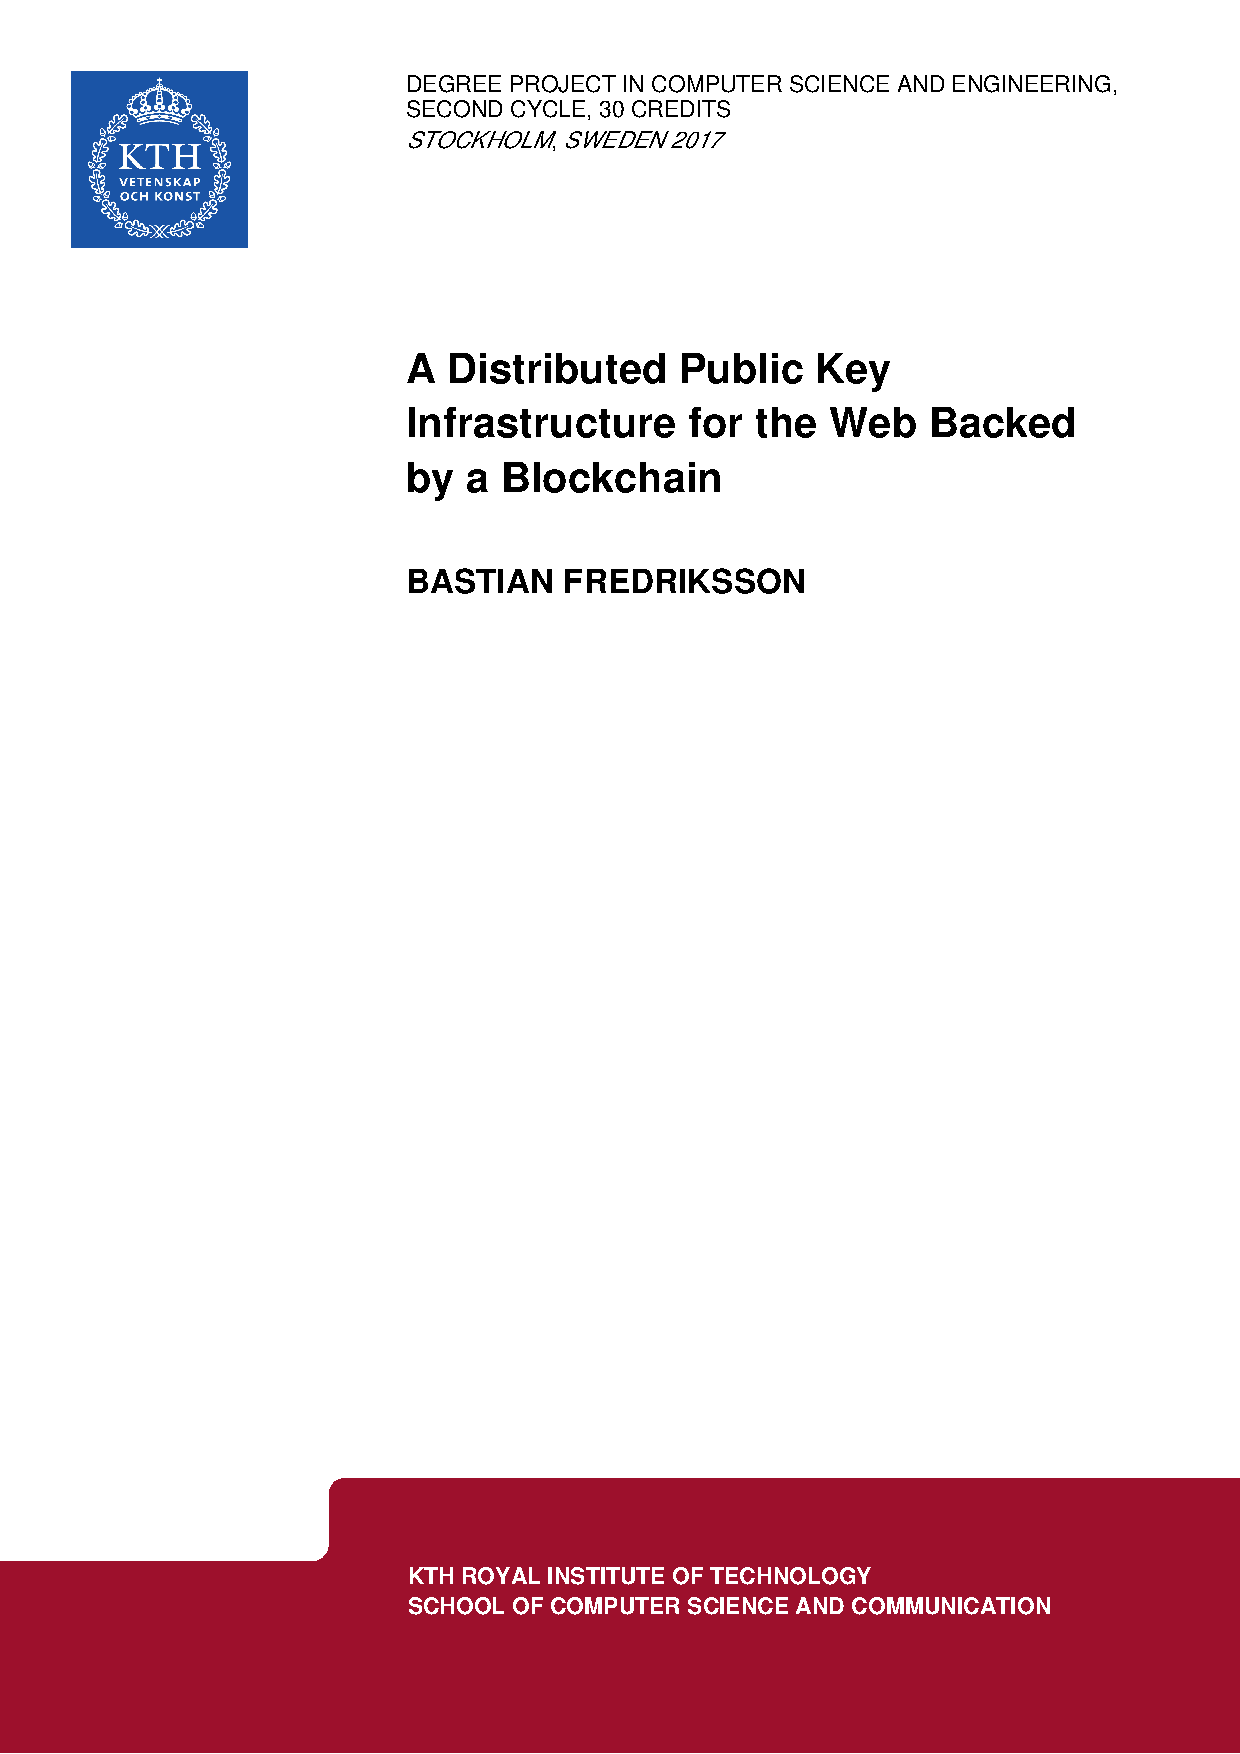
\includepdf[pages={1}]{cover/front.pdf}
\frontmatter
\titlepage
\section*{Abstract}
The thesis investigates how a blockchain can be used to build a decentralised public key infrastructure for the web, by proposing a custom federation blockchain relying on honest majority. Our main contribution is the design of a Proof of Stake protocol based on a stake tree, which builds upon an idea called follow-the-satoshi used in previous papers.

Digital identities are stored in an authenticated self-balancing tree maintained by blockchain nodes. Our back-of-the-envelope calculations, based on the size of the domain name system, show that the block size must be set to at least 5.2 MB, while each blockchain node with a one-month transaction history would need to store about 243 GB. Thin clients would have to synchronise about 13.6 MB of block headers per year, and download an additional 3.7 KB of proof data for every leaf certificate which is to be checked.
\section*{Sammanfattning}
Uppsatsen undersöker hur en blockkedja kan användas för att bygga en decentraliserad publik nyckel-infrastruktur för webben. Vi ger ett designförslag på en blockkedja som drivs av en pålitlig grupp av noder, där en majoritet antas vara ärliga. Vårt huvudsakliga bidrag är utformningen av ett Proof of Stake-protokoll baserat på ett staketräd, vilket bygger på en idé som kallas follow-the-satoshi omnämnd i tidigare publikationer. 

Digitala identiteter sparas i ett autentiserat, självbalanserande träd som underhålls av noder anslutna till blockkedjenätverket. Våra preliminära beräkningar baserade på storleken av DNS-systemet visar att blockstorleken måste sättas till åtminstone 5.2 MB, medan varje nod med en månads transaktionshistorik måste spara ungefär 243 GB. Webbläsare och andra resurssnåla klienter måste synkronisera 13.6 MB data per år, och ladda ner ytterligare 3.7 KB för varje användarcertifikat som skall valideras.
\ifbook
\clearpage
\fi
\section*{About PrimeKey}
This thesis was written at \textbf{PrimeKey Solutions AB}. PrimeKey provides businesses and organisations around the world with the ability to implement security solutions such as e-Passports, authentication, digital signatures, unified digital identities and validation using EJBCA Enterprise, SignServer Enterprise and PrimeKey PKI Appliance. PrimeKey has its head office in Stockholm, Sweden.
\ifbook
\clearpage
\fi
\section*{Acknowledgements}
I want to thank PrimeKey for giving me the opportunity to write this thesis, specifically Johan Eklund and my PKI advisor Mike Kushner who have taken great interest in my work and provided me with useful feedback. I also want to thank everyone at my university who have helped me throughout the writing of this thesis, most notably my university advisor Dr. Per Austrin and my examiner Prof. Johan Håstad. I also want to mention the following students who have helped me peer review an earlier draft: Arash Safari, Edvin Lundberg, Hannes Leskelä, Lovisa Runhem and Martin Steier - thank you for your ideas and comments! Finally, I want to thank Dimaz Ankaa Wijaya for all interesting conversations about blockchains. 
\cleardoublepage
\else
\title{A Distributed Public Key Infrastructure for the Web Backed by a Blockchain}
\author{
  Bastian Fredriksson\\
  PrimeKey Solutions AB\\
  Lundagatan 16\\
  171 63 Solna, Stockholm\\
  \texttt{bastian@primekey.com}
}
\twocolumn[
  \begin{@twocolumnfalse}
    \maketitle
    \begin{abstract}
      The binding between a physical identity and a public key is an important building block in computer security. This is typically done through digital documents following the X.509 standard, named X.509 certificates. These certificates are signed with the private key of a trusted intermediary called a certificate authority, who is responsible for checking the identity of the customer before issuing the certificate. Unfortunately, certificate authorities sometimes fail in their duty and issue fraudulent certificates. This violates the centralised trust model and makes it hard to trust any certificates issued by such certificate authority. One way of solving this problem is to adapt a decentralised model, where each user cross-signs their certificate with their private key. In such a system, a problem of consensus arises: How can we know which key is associated with a certain user? The emergence of the blockchain, originally used to store transactions for the Bitcoin cryptocurrency, offers a possibility to solve this problem without relying solely on a certificate authority. The aim of the thesis is to investigate how a blockchain can be used to build a decentralised public key infrastructure for the web, by proposing a custom federation blockchain which stores digital identities in an authenticated tree structure. Our main contribution is the design of a Proof of Stake protocol based on a stake tree which builds upon an idea called follow-the-satoshi used in previous papers. Our back-of-the-envelope calculations based on the size of the domain name system suggest a block size of at least 5.2 MB, while each blockchain node with a one-month transaction history need to store about 243 GB. Thin clients would have to synchronise about 13.6 MB of block headers per year, and download an additional 3.7 KB of proof data for every leaf certificate which is to be checked.
    \end{abstract}
  \end{@twocolumnfalse}
  ]
\fi

\ifbook
\tableofcontents
\mainmatter
\newcommand{\comma}[0]{, }

\begin{filecontents*}{glossary.csv}
%termID                           , description
Public key infrastructure (PKI)   , A set of entities\comma policies and procedures used to issue\comma manage and revoke $(\text{name}\comma \text{key})$ pairs used for authentication.
Public key                        , The public component of a cryptographic keypair. The public key can be used to verify a digital signature created using the corresponding private key.
Certificate authority (CA)        , An entity responsible for signing digital \emph{certificates}.
Digital signature                 , A cryptographic fingerprint created using a signature algorithm. A digital signature can be used to check the authenticity of a document\comma such as a \emph{certificate}.
Certificate                       , A signed digital document which binds a name to a \emph{public key}.
Altcoin                           , An umbrella term for all non-Bitcoin cryptocurrencies.
Key bridging                      , A technique used by routers to inspect TLS traffic. A benevolent form of a \emph{man-in-the-middle attack}.
Transport Layer Security (TLS)    , A protocol used to establish an authenticated and encrypted connection over the Internet.
Identity retention                , A desirable property of a \emph{public key infrastructure}\comma where an identity cannot be changed without the consent of its owner.
Man-in-the-middle attack          , An attack where an adversary sits between a server and the victim\comma intercepting all traffic between them.
Smart contract                    , An escrow operation stored on and executed by nodes operating a blockchain.
Root Certificate Authority (Root CA) , A \emph{certificate authority} with a self-signed certificate\comma typically trusted by all major web browsers and operating systems.
Intermediary Certificate Authority (Intermediary CA) , A \emph{certificate authority} with a certificate signed by a \emph{root certificate authority}.
Double spending attack            , An attack against a cryptocurrency\comma where the same money is spent twice.
Mempool                           , A memory pool of pending transactions awaiting to be included in a block on the blockchain.
Keyblock                          , A block in Bitcoin-NG signalling the change of \emph{block leader}.
Microblock                        , A block in Bitcoin-NG\comma containing transactions\comma generated by the current \emph{block leader}.
Block leader                      , A blockchain node eligible to approve transactions and adding blocks to the blockchain.
Truststore                        , A file containing trusted \emph{certificate authorities} and their \emph{public keys}.
Longest chain                     , The blockchain currently considered to be the ``correct'' chain by the blockchain network.
Block reward                      , Cryptocurrency paid to a \emph{miner} for adding a new block to the blockchain.
Coinbase transaction              , The first transaction in a block. Contains the address which receives the block reward.
Merged mining                     , A technique used by \emph{miners} to mine on more than one blockchain at a time.
Satoshi                           , The smallest unit of cryptocurrency which can be transferred between two wallets.
Follow-the-satoshi                , A technique used in \emph{Proof of Stake} to derive a \emph{block leader} by sampling a random \emph{satoshi}.
Proof of Stake                    , A blockchain \emph{consensus protocol} where ownership of cryptocurrency is the foundation for participation in the consensus process.
Simple Payment Verification (SPV) , A technique which allows a blockchain client to verify a transaction without downloading the whole blockchain.
Unspent Transaction Output (UTXO) , A set of transactions not yet referred to by other transactions. Determines the balances of wallets.
Public key pinning                , A security feature whereby a web client associates a \emph{public key} with a web server.
Certificate Transparency (CT)     , A system of public logs containing certificates issued by a \emph{certificate authority}\comma used to detect misissuance and fraudulent \emph{certificates}.
Merkle root hash                  , The hash found in the root of a Merkle tree. Comprises a compact representation of all nodes in the tree.
Domain Name System (DNS)          , A catalog service used to map an IP address to a domain name.
Certificate Signing Request (CSR) , A document sent to a \emph{certificate authority}\comma in order to apply for a \emph{certificate}.
Registration Authority (RA)       , An entity acting on behalf of a \emph{certificate authority}\comma authorised to apply for\comma reject and revoke \emph{certificates}.
Domain Validated Certificate (DV) , A \emph{certificate} obtained after proving ownership of a domain name.
Organisation Validated (OV) Certificate, A type of \emph{certificate} issued to organisations.
Extended Validation (EV) Certificate, A type of \emph{certificate} issued to organisations. Involves more scrutiny than an \emph{OV certificate}.
Automatic Certificate Management Environment (ACME), A challenge-response protocol automating the issuance of \emph{DV certificates}.
Distinguished Name (DN)           , The field in a \emph{certificate} containing owner of the \emph{public key}.
OCSP responder                    , A entity acting on behalf of a CA\comma responsible for checking the validity of \emph{certificates} by responding to queries over the OCSP protocol.
OCSP stapling                     , A technique whereby a server bundles an OCSP response with the certificate during the TLS handshake.
Consensus algorithm               , An algorithm which allows a network\comma partly consisting of malicious actors\comma to agree on a result. See \emph{Byzantine Generals' Problem}.
Fork (blockchain)                 , The name of two blockchains with the same length. A fork occurs when two blocks are created at approximately the same time.
Byzantine Generals' Problem       , A consensus problem\comma formulated in a 1982 paper \cite{Lamport82}\comma  where a set of generals try to agree on whether they should attack a city. 
Miner                             , An entity in the blockchain network trying to become the next \emph{block leader}\comma by performing computationally intensive tasks. See \emph{Proof of Work}.
Trapdoor function                 , A function in cryptography which is easy to verify\comma but hard to reverse.
Validation authority (VA)         , An entity authorised to provide revocation services on behalf of a CA.
Sybil attack                      , A type of attack against a reputation system where security is subverted by forging a large number of identities in a P2P-network. 
Multisignature (multisig) script  , A type of Bitcoin script which requires signatures from multiple public keys. One example of a multisignature scheme is Shamir Secret Sharing \cite{Shamir79}.
Label (DNS)                       , A part of a DNS domain name separated with a dot.
Object Identifier (OID)           , An identifier mechanism standardised by the International Telecommunications Union (ITU) and ISO/IEC for naming any an object (such as an algorithm\comma entity of datastructure) with a globally unambiguous name.
Full blockchain node              , A blockchain node which enforces all rules of the blockchain protocol by downloading\comma verifying and archiving every block and transaction.
Pruning node                      , A \emph{full blockchain node} which throws away old blocks and transactions to reclaim disk space.
SPV node                          , A blockchain node which does not enforce all the rules of the blockchain protocol. An SPV node typically only downloads and verifies the block headers of the longest blockchain.
Thin client                       , See \emph{SPV node}.
Bitcoin miner                     , See \emph{miner}.
Proof of Work                     , A blockchain \emph{consensus protocol} based on problems which require a lot of computing power to solve.
Internet Corporation for Assigned Names and Numbers (ICANN), Non-profit organisation responsible for the maintenance and registration of domain names. 
\end{filecontents*}


\DTLloaddb[noheader,keys={termID,description}]{words}{glossary.csv}
\DTLsort{termID=ascending}{words}
\renewcommand{\arraystretch}{1.5}
\chapter*{Glossary}
\begin{longtable}{l>{\raggedright\arraybackslash}p{.4\textwidth} p{.6\textwidth}}
  \DTLforeach{words}{
    \termID=termID,\termdesc=description}{
    & \textbf{\textit{\termID}} & \termdesc \\
  }
\end{longtable}
\else
\twocolumntoc
\fi

\chapter{Introduction}
There are countless of electronic devices around us, ranging from desktop computers and servers to smartphones and e-Passports. Many of these devices need a digital identity which can be verified as legitimate. Without a trusted digital identity, there is no way of authenticating the remote party, and it becomes impossible to establish a secure communication channel. Digital identity is most commonly managed using something called certificates, a digital document containing an identifier, a \emph{public key} and a \emph{digital signature} created by a trusted \emph{Certificate Authority (CA)}. If the communication is facilitated over the Internet, the identifier is usually an IP-address or a domain name which can be resolved through DNS. The validity of the information in the certificate can be checked by inspecting the signature of the CA using the CA's public key. The CA's public key is stored in a file (which is typically bundled with the operating system or the web browser) containing a list of trusted CAs and their corresponding public keys.

There are some problems with this centralised trust model. The use of a CA introduces a single point of failure, and history has shown us that we put too much trust in the CAs. A CA might issue the wrong type of certificate by mistake, as shown by the TürkTrust incident in mid 2011, where the Turkish certificate authority TürkTrust issued two intermediary CA certificates instead of regular certificates. One of these certificates was revoked immediately after a request from the customer, but the other certificate issued to EGO, a public transport company in Ankara, was not revoked. EGO now had the power to act as a CA by signing certificates on behalf of TürkTrust. At the end of 2012, EGO implemented an HTTP proxy for outgoing HTTPS traffic, where they used their intermediary certificate for \textit{key bridging}. The fraudulent intermediary certificate was detected after users started to get warnings when visiting $\mathsf{google.com}$, a domain which used \emph{public key pinning}, a technique which allows a web browser to detect if the public key used by a domain has changed \cite{Ducklin13}.

A CA might also be compromised by an adversary, which happened in March 2011 when a self-proclaimed Iranian hacker compromised two resellers of Comodo certificates. The hacker successfully signed nine different certificates for seven different domains, including Skype, Yahoo, Mozilla's web store and Google's Gmail \cite{Leyden11}. In September the same year, the Dutch CA DigiNotar was declared bankrupt after at least 531 fraudulent certificates had been issued. The fraudulent certificates were used to perform \emph{man-in-the-middle attacks} on Google's services \cite{Fox11}.

A server can be linked to several digital identities, which makes it more difficult to differentiate between a legitimate identity and a counterfeit one. Several attempts to fix this problem has been made. One such attempt is public key pinning where a server sends a fingerprint of its public key, or the public key of the CA certificate to the client. The fingerprint is stored by the client, which makes it possible to detect if the key changes in the future. Pinning has unfortunately not been widely adopted, possibly because it requires configuration of the web server, and because pinning poses a risk to domain holder. Customers who are not visiting the domain for the first time expects the certificate to contain a previously pinned key. If the domain holder loses access to these keys, or if the keys become compromised, the browser rejects the connection, and the customer is unable to visit the site. Similarly, pinning the public key of the CA acts as a lock-in mechanism since it makes it more difficult for the domain holder to switch CA.

Another approach is \emph{Certificate Transparency (CT)}, which aims to detect fraudulently issued certificates by forcing CAs to append certificates being issued to a certificate transparency log. These logs can then be monitored by a third party such as the domain holder. While certificate transparency has indeed helped to detect malicious certificates in some cases, the lack of incentive for third parties to audit the logs raises concerns for how efficient certificate logs are for average users. But more importantly, Certificate Transparency does not prevent a fraudulent certificate from being issued in the first place.

An alternative to a \emph{Public Key Infrastructure (PKI)} based on CAs is \emph{Web of Trust}. In Web of Trust, there is no central authority which is vouching for an identity, and thus there is no central point of failure. Instead, users are responsible for verifying the identity of the people they want to communicate with or trust other people to do so. After asserting the validity of a certain public key, it is imported to the user's keyring. Keys might be posted on the web or exchanged in person. Web of Trust is standardised in the OpenPGP standard \cite{RFC4880} and is integrated into Linux package managers and some email programs. Unfortunately, Web Of Trust might be somewhat cumbersome to use. Each key must be verified before being inserted into the keyring, and a compromised key must be manually removed. Similar to public key pinning, Web of Trust also fails to offer any built-in mechanism for key recovery and lacks some restriction metadata that certificates can provide like extended key usages and name constraints.

A blockchain, an append-only, public ledger, originally designed to store transactions for the Bitcoin cryptocurrency \cite{Nakamoto08}, has been used to implement a wide variety of decentralised applications, such as smart contracts \cite{Wood14}, decentralised cloud storage \cite{Wilkinson14}, asset tracking \cite{Rosenfeld12}, and distributed databases \cite{McConaghy16}. Another potential use case for blockchains could be as a distributed PKI, and this is what is investigated in this thesis. A blockchain could offer built-in certificate transparency, and allow pinning of both public keys and certificates. Each computer in a large P2P-network has its own copy of the blockchain, which allows each client to independently verify each transaction, removing the single point of failure.

\section{Problem Statement}
\begin{itemize}
    \item[~] \textit{Are blockchains suitable as a building block for a distributed public key infrastructure and what could such a public key infrastructure look like?}
\end{itemize}

\section{Motivation and Aim}
The motivation behind this thesis is to secure digital communications by improving \emph{identity retention} in the current PKI. This is an important problem, since the current PKI based on CAs is the technology underpinning many security critical applications on the Internet, such as electronic commerce, online banking and software updates. Improvement in this area is of great interest for anyone relying on, or otherwise dealing with certificates, perhaps most notably CAs and domain owners. We believe that the problem of fraudulent certificates, which has been plaguing users for years, stems from the inherent centralisation of the current system based on trusted certificate authorities, which have the power to issue certificates on behalf of users without their consent. Although the need for trusted entities which bind a physical identity to a digital one is recognised, we believe CAs have been given an unfavourable role with too much responsibility. With this in mind, a complementary solution is proposed where identities are stored in a public ledger, which is maintained by an honest majority instead of a central authority, with the aim of creating a versatile and more robust PKI.

We believe a blockchain in a P2P-setting, similar to Bitcoin, to be a suitable building block for a public ledger, for multiple reasons:

\begin{itemize}
    \item[\checkmark] \textbf{Tamper-proof} Transactions performed on the blockchain are hard to reverse, making it difficult to impersonate someone.
    \item[\checkmark] \textbf{Offers consensus} It provides a robust mechanism for consensus, even in the presence of malicious adversaries.
    \item[\checkmark] \textbf{Incentive based} There is a possibility for incentivising participation in the network.
    \item[\checkmark] \textbf{Transparent} All transactions are public and can be verified independently by all nodes in the network.
    \item[\checkmark] \textbf{Programmable} Built-in support for scripts, which allows for advanced key recovery mechanisms.
    \item[\checkmark] \textbf{Censorship resistant} Direct node communication makes the network resilient against denial of service.
\end{itemize}

\section{Delimitation}
This thesis is supposed to act as a blueprint, similar to that of an Internet draft, for the design of a distributed PKI aimed for the web. As such, our work is mostly theoretical. Focus is on the design of the blockchain, the consensus process and the format of transactions. Procedures for issuance and revocation of digital identities, and how clients can verify certificates in our system, are only covered very briefly. The blockchain network protocol is not be discussed. The choice of stakeholders (the entities responsible for maintaining the blockchain), or under what circumstances stakeholders should be excluded from the consensus process is considered beyond the scope of this thesis.

\section{Thesis Content and Contribution}
\cref{chap:background} contains a background study about PKIs and blockchains. \cref{chap:method,chap:blockchain} describes the design of the blockchain, including a two-phase Proof of Stake protocol which selects block leaders from a stake tree, and the use of an account tree which stores the public keys of domain owners. \cref{chap:identity} focuses on approval and issuance of new identities. To achieve our goal, two new certificate extensions are proposed. The first certificate extension, the CA proof, contains the information needed by blockchain nodes to verify new accounts which should be added to the account tree. The second certificate extension contains a server signature produced by the domain owner's public key, and is used by compatible clients to verify certificates presented to them. \cref{chap:evaluation} contains a security and performance analysis of this blockchain scheme, where we look at different security threats and how our scheme would scale if deployed on the same scale as DNS. Finally, we conclude and identify future work in \cref{chap:discussion}.

\section{Choice of Methodology}
Our methodology is roughly based on the following four activities:
\begin{itemize}
    \item \textit{Problem identification} Define the problem to be solved and explain why this problem is important. This step is conducted by a background study. 
    \item \textit{Define objectives for a solution} This is done by identifying limitations of existing solutions based on the background study.
    \item \textit{Design a solution} Propose a distributed PKI which aims to satisfy the previously defined objectives.
    \item \textit{Evaluate the solution} Discuss and analyse the solution and identify weaknesses and areas of future work.
\end{itemize}

\section{Related Work}
Previous work on the use of blockchains in distributed PKIs is sparse, although there are several approaches to log-based certificate management without an underlying blockchain \cite{Basin14, Kim13, Yu14, RFC6962}. The works discussed in this section are \emph{Namecoin} - a distributed DNS based on Bitcoin, \emph{Blockstack} - a blockchain-agnostic PKI and DNS currently running on top of the Bitcoin blockchain, \emph{Instant Karma PKI} - a certificate transparency log powered by smart contracts, and coloured coins - a way of tracking digital assets on a blockchain.

\subsection{Namecoin}
The use of a blockchain as a storage medium for digital identities was introduced together with Namecoin \cite{Kalodner15}, which became the first fork of the Bitcoin software. It was the first secure, distributed naming system to offer human-memorable names, which was conjectured to be impossible\footnote{See Zooko's triangle: \url{https://en.wikipedia.org/wiki/Zooko\%27s\_triangle}.}. Namecoin runs its own blockchain using \emph{Proof of Work} as consensus mechanism, but lends some of its hashing power from other \emph{Bitcoin miners} via a mechanism called \emph{merged mining}.

Namecoin administers its own $\mathsf{.bit}$ top domain independently from \emph{The Internet Corporation for Assigned Names and Numbers (ICANN)}. New names are registered in this namespace by posting a message to the Namecoin blockchain. Names expire after 36000 blocks (about 250 days) but once a name is registered, it can only be transferred or renewed by the person or organisation who currently owns it. Thus, Namecoin is completely censor-resistant and no central authority has the power to remove existing names. Blockchain nodes enforce fees associated with name registration and renewals, and any name can be registered as long as it is vacant.

\subsection{Blockstack}
Blockstack \cite{Ali16} works as both a PKI and a DNS, and allows users to register zonefiles which contains a public key and a pointer to the user's profile. The profile is a signed JSON document which can contain any type of information associated with the specific user. The profile can be stored at a cloud service provider, or on a server administered by the user. The hash of the zonefile is written in an $\mathsf{OP\_RETURN}$ transaction on the Bitcoin blockchain, while the zonefiles themselves are stored in a distributed filesystem maintained by Blockstack nodes. Blockstack is blockchain-agnostic which means that it is possible to migrate to another blockchain if required. Blockstack achieves this by the use of a \emph{virtualchain}, created by Blockstack nodes by filtering and parsing the underlying blockchain.

\subsection{Instant Karma PKI}
Instant-Karma PKI (IKP) \cite{Matsumoto16} is an attempt to improve Certificate Transparency by incentivising participants to look for and report fraudulent certificates. The goal of IKP is to incentivise, decentralise and automate processes for handling CA misbehaviour. This is done by leveraging the Ethereum's support for smart contracts\footnote{Ethereum is a blockchain-based platform for building decentralised applications. More information is available at: \url{https://www.ethereum.org/}}. An IKP contract takes a certificate as input, provided by a monitor, and checks this certificate against a Domain Certificate Policy which specifies a list of CAs allowed to issue certificates for this particular domain. If the certificate is issued by a CA not present in this list, a Reaction Policy is executed which performs the escrow operation transferring Ether (Ethereum's cryptocurrency) from the misbehaving CA to the affected user and the monitor who reported the violation.

\subsection{Coloured Coins}
Coloured coins is a family of protocols used for tracking ownership of digital or physical assets on a blockchain. Coloured coins can be used to build tamper-proof land registers \cite{Lantmateriet16}, reduce counterfeits in for example the sneaker, wine and medical industries, track ownership of diamonds, and secure the integrity of trade documents \cite{Infosys16}. There are several implementations of the coloured coins concept, for example Open Assets, ChromaWallet, CoinSpark and Colu.

The idea behind coloured coins is as follows: An asset is represented by a set of coins on the blockchain which are equipped with some metadata, or more specifically by a transaction output as described in \cref{blockchain-transactions}. By traversing the blockchain, one can follow the chain of ownership for these coins, and establish consensus for the current owner of an asset.

The asset can then be transferred between owners by spending the coins. This transaction of ownership can be done without involving any central authority, since the blockchain is completely decentralised. If the transfer of ownership is made between two people who do not trust each other, one typically employs a trusted intermediary, such as a broker which carries out an escrow. However, blockchains do not require an intermediary to facilitate a trusted escrow, even if the participants are malicious. Bitcoin's script support, or the use of more sophisticated smart contracts allows the transfer of ownership to be executed in a single atomic transaction, which makes it impossible to cheat \cite{Rosenfeld12}. If a physical asset is to be associated with a digital identity, one typically needs a trusted authority, for example a CA, responsible for maintaining a mapping between an asset and the corresponding output on the blockchain. This mapping can be stored in a file, signed with a notary's private key, and the integrity of the file can be ensured by storing a hash of the file on the blockchain \cite{Mizrahi17}.

\subsection{Limitations of Existing Solutions}
Existing blockchain-based PKIs such as Namecoin and Blockstack have their shortcomings: they lack integration with the existing PKI and are not ownership consistent with DNS which makes them difficult to adapt. It is also doubtful whether a system such as Namecoin or IKP could be deployed on a global scale due to scalability issues. The team behind Blockstack has considered the use of autonomous subdomains maintained off-chain to improve scalability, but this is may not be a viable solution for many domain holders. Existing blockchains based on Proof of Work are also facing issues with poor distribution of hashing power in the network. Blockstack was originally deployed on top of the Namecoin blockchain, but they switched to the Bitcoin blockchain after a security problem was detected where a single miner controlled more than half the hashing power in the network for an extended period of time \cite{Ali16}. Although coloured coins can be used to track certificates or domain name ownership, they require a client to verify the transaction history of the coin which can be impractical for low-powered devices.

\chapter{Background}
\label{chap:background}
This chapter establishes a firm theoretical foundation for the rest of the thesis. Topics covered include Merkle trees, the basics of X.509 certificates, as well as the role of CAs in the PKI ecosystem and some attempts to improve the transparency and security of the current PKI.

Finally we move on to the main topic of this thesis, namely blockchains, where Bitcoin's transaction model, some consensus algorithms, and proposals for improving the scalability and efficiency of the blockchain are explained. Our starting point is the Bitcoin blockchain, which is the most influential blockchain today.

\section{Merkle Trees}
\label{merkle-tree}
Merkle trees, also known as Merkle hash trees or binary hash trees, were first described in \cite{Merkle87} in the context of digital signatures. A Merkle tree is a useful cryptographic primitive when one wants to prove the existence of a record within a set. One can construct a (static) Merkle tree from a set of records by hashing each record in the set and let these hashes be the leafs in a binary tree. Each parent node is constructed by combining the hashes of its two child nodes, usually by hashing the concatenation of the two.

Thus, the hash of each parent node comprises a compact representation of its two child nodes. Given a (trusted) hash for the root of the Merkle tree, known as a \emph{Merkle root hash}, one can prove that a certain leaf node is present in the tree by providing the $\mathcal{O}(\log n)$ hashes needed to reconstruct the Merkle root hash. To give a proof for a leaf node not in the tree is as hard as finding a collision in the underlying hash function \cite{Coronado05}. \cref{fig:merkle-tree} shows an example of a static Merkle tree.

More formally, consider a tree of depth $d$, where each of the $N_i$ nodes contains a hash $N_i.\mathsf{hash}$. Given a list of records $\mathbb{L}$ with size $|\mathbb{L}|=2^d, d\in \mathbb{Z}_{+}$ we create a static Merkle tree from a collision resistant hash function $H$ as follows: Create a list of hashed records $\mathbb{L}_H = [H(x), x \in \mathbb{L}]$ and put these hashes in the $2^{d}$ leaf nodes $N_{2^{d}}\ldots N_{2^{d+1}-1}$ of the tree. Then construct the rest of the tree in a bottom-up fashion, using the following rule:

\begin{equation}
    N_i.{\mathsf{hash}} = H(N_{2i}.\mathsf{hash} \text{ | } N_{2i+1}.\mathsf{hash})
\end{equation}

To prove the existence of a record, one should provide the hashes stored in the sibling nodes for the nodes traversed along the path down to a particular leaf. Additionally, one needs to know whether each hash was stored in a left sibling node (0) or a right sibling node (1). Thus, to prove the existence of record whose hash is stored in the leaf node $i \in [2^{d}, 2^{d+1}-1]$, compute the indices $\mathbb{I} = [ \text{sibling}(\floor{\frac{i}{2^n}}), n \in \mathbb{Z}_d]$ and finally the tuples $\mathbb{P} = [ (i \mod 2, N_i.\mathsf{hash}), i \in \mathbb{I} ]$.

\[
  \text{sibling}(i)=\begin{cases}
               i + 1 ~\textit{when i is even}\\
               i - 1 ~\textit{when i is odd}
            \end{cases}
\]

The cryptographic proof $\mathbb{P}$ is called a \textit{Merkle proof} and is used to prove membership of a record without large storage or bandwidth requirements. Some variants of Merkle trees, such as Sparse Merkle trees \cite{Dahlberg16} also allows for efficient non-membership proofs.

\subsection{Dynamic Merkle Trees}
\label{sec:dyn-merkle}
To obtain a Merkle tree which can be efficiently updated when new nodes are added or removed, it may be advantageous to associate not only the leaves, but also interior nodes of the tree with a record. Each node $N_i$ in this tree contains two hashes instead of one, the Merkle hash $N_i.\mathsf{merkleHash}$ and the hash $N_i.\mathsf{dataHash}$ of the associated data record. The Merkle hash of every touched node is then recomputed when the tree is rotated as follows:

\begin{equation}
\begin{split}
    N_i{\mathsf{.merkleHash}} = H(N_i\mathsf{.dataHash} \text{ | } \\ N_i\mathsf{.leftChild.merkleHash} \text{ | } \\ N_i\mathsf{.rightChild.merkleHash})
    \end{split}
\end{equation}

The Merkle hash of a non-existent child node (for example if $N_i$ is a leaf) can be set to $0$ or some other fixed hash denoting the end of a branch. To prove the existence of a record in the tree, one need to provide the $\mathsf{dataHash}$ and the $\mathsf{merkleHash}$ of the correct child node for each level in the tree. An example of a dynamic Merkle tree is the IAVL+ Tree which is rotated on updates using a variant of the AVL algorithm \cite{Tendermint15}.

\begin{figure*}[ht!]
    \centering
    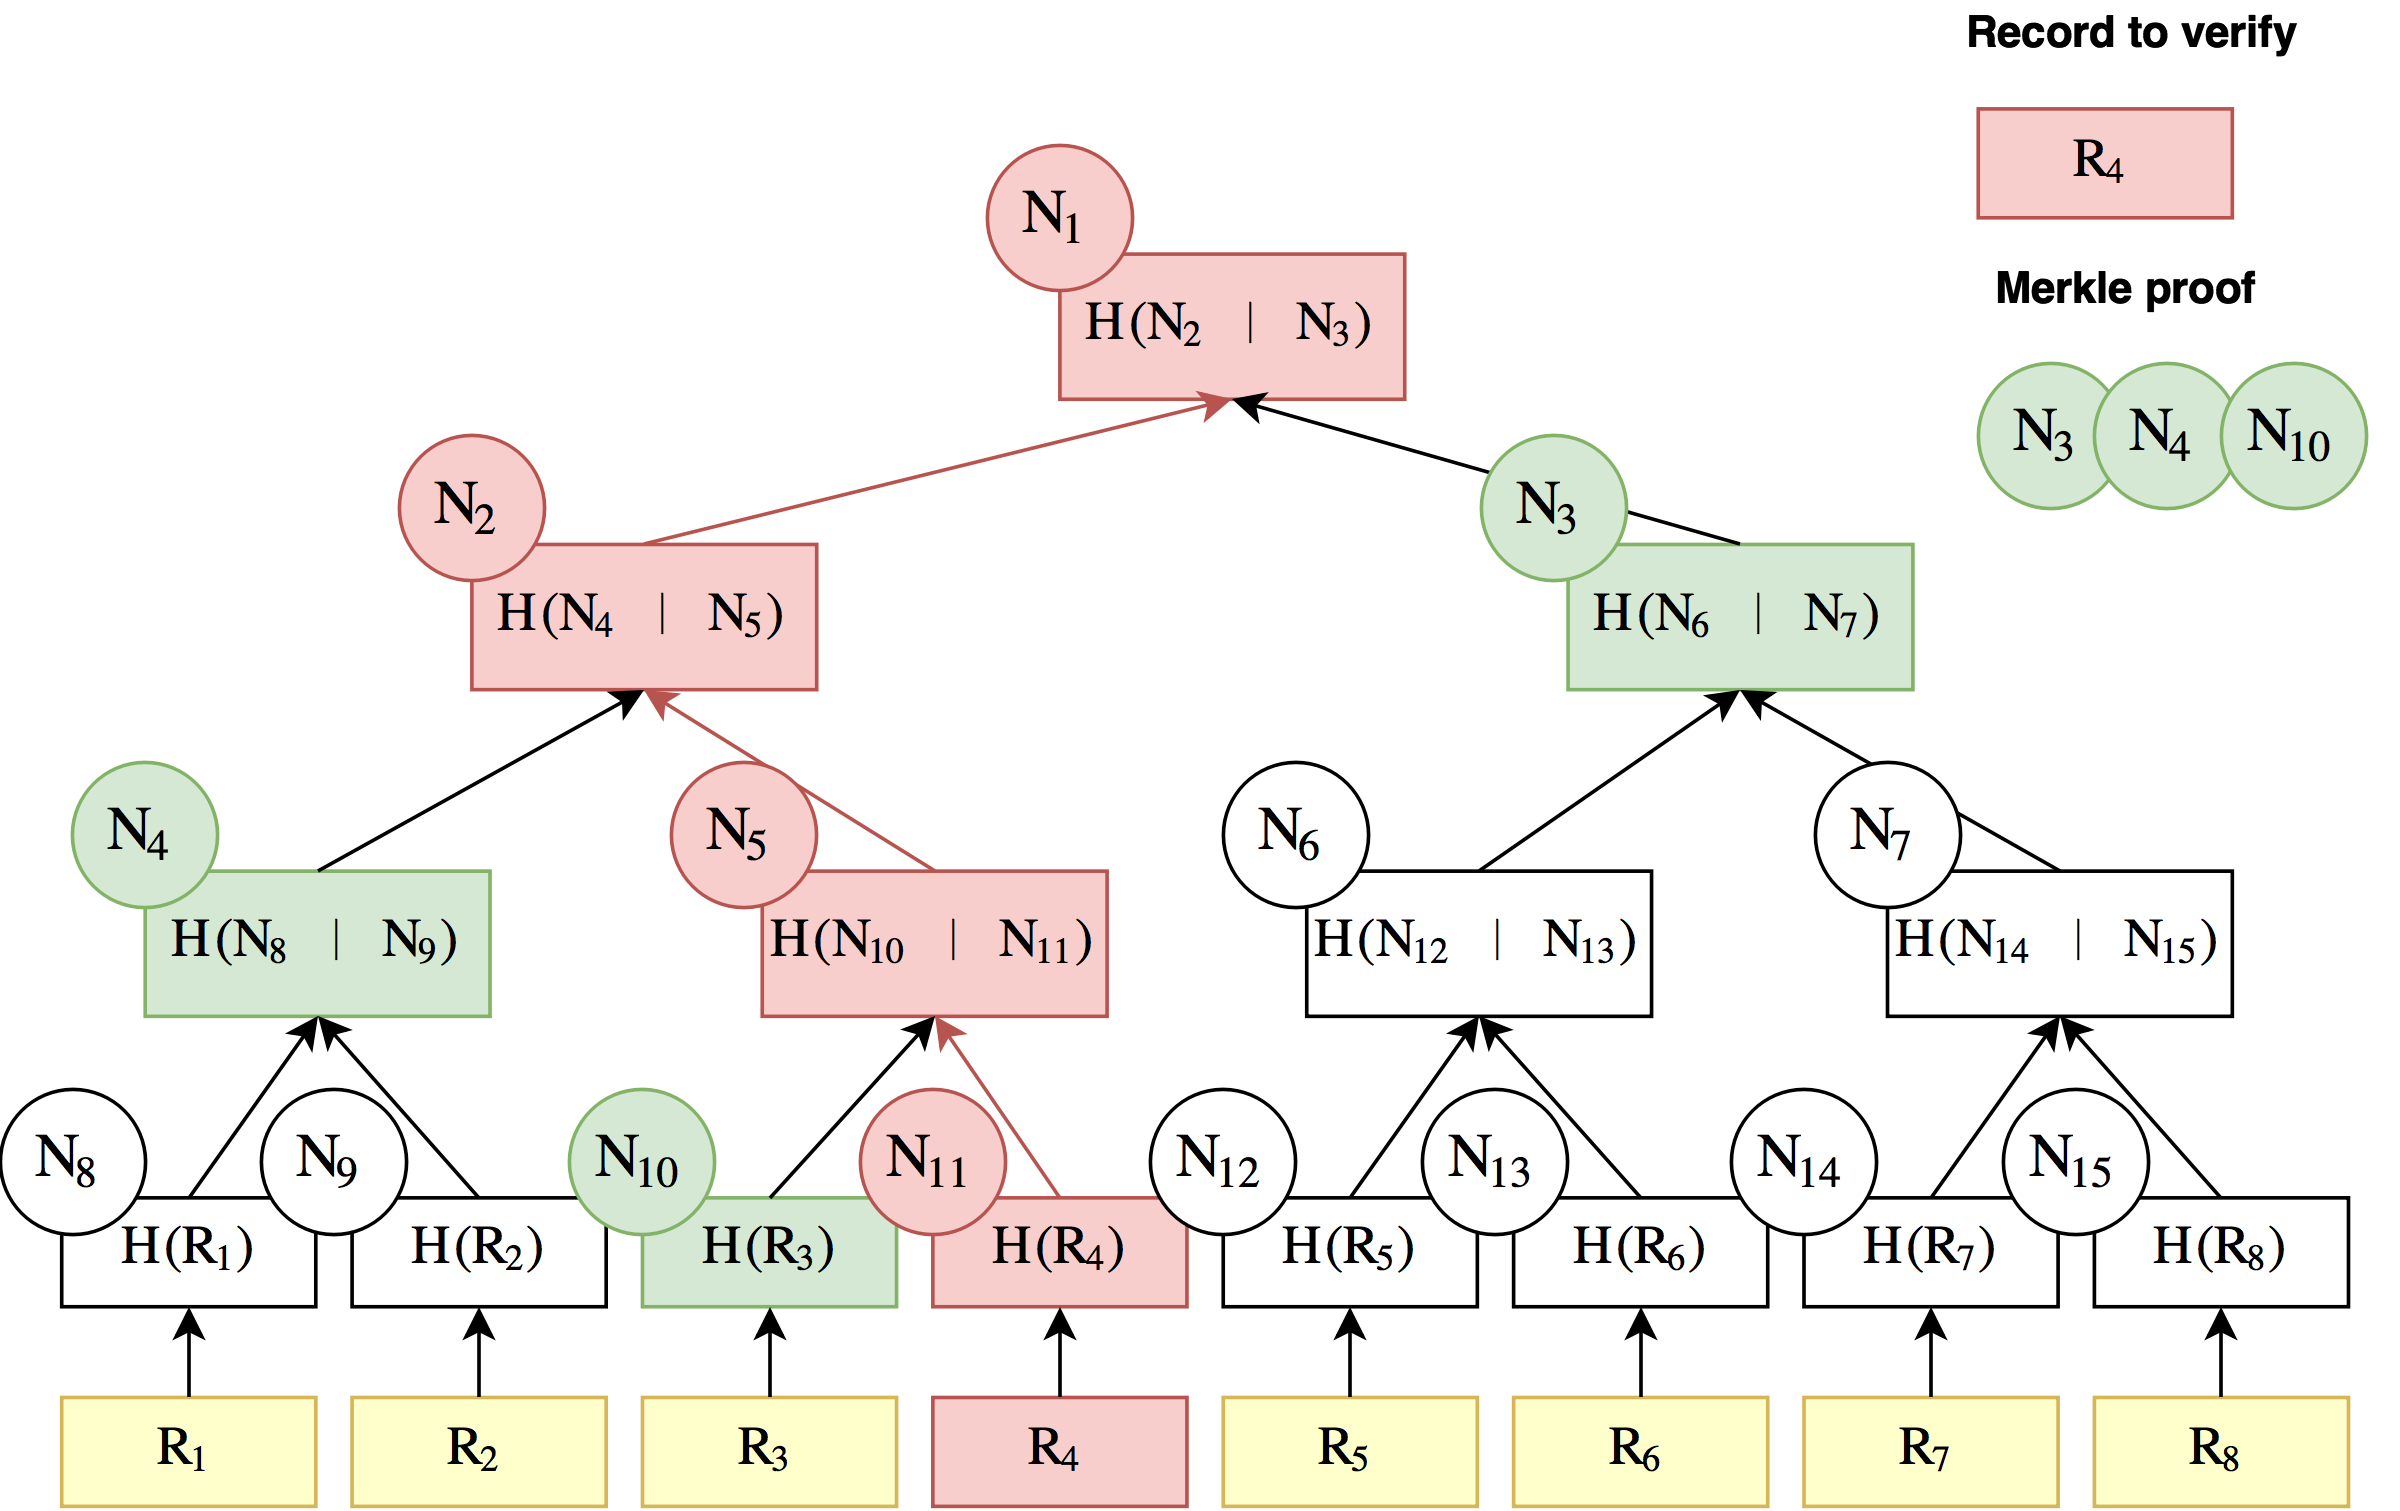
\includegraphics[width=\textwidth]{figures/merkle-tree}
    \caption{A Merkle tree with 15 transactions. The nodes in the Merkle proof used to verify the transaction hashed into node 11 are coloured in green.}
    \label{fig:merkle-tree}
\end{figure*}

\section{Public Key Infrastructure}
In this section we cover the basics of an X.509 public key infrastructure (X.509 PKI), a PKI with one or more trusted certificate authorities who are binding names to keys by issuing certificates in the X.509 format. For clarity, we start this chapter by repeating two definitions from the glossary.

\begin{definition}[Public key infrastructure]
A public key infrastructure is a set of entities, policies and procedures used to issue, manage and revoke $(\text{name}, \text{key})$ pairs used for authentication.
\end{definition}

\begin{definition}[Certificate]
A certificate is a signed digital document which binds a name to a public key.
\end{definition}

\subsection{Certificate Authorities}
The certificate authority (CA) is the entity responsible for issuing certificates. These certificates are signed by the CA, and relying parties can check the validity of the signature using the corresponding public key stored in a file, called the \emph{truststore}. Certificate authorities can usually be either a \emph{root CA} or an \emph{intermediary CA}. The root CA issues a certificate to the intermediary CA, which allows the intermediary CA to sign certificates on behalf of the root CA. This is a common practice, and is done both for practical and security reasons. There are typically many different intermediary certificate authorities, with different trust levels, issuing different types of certificates. For all intermediary CAs acting on behalf of the same root CA, only one certificate needs to be stored in the client's truststore, namely the certificate of the root CA, called the root certificate. The root CA is typically kept offline, unless it is needed to create or revoke an intermediary CA. This adds an extra layer of security, since if the intermediary CA gets compromised, which could happen if an adversary gets hold of their private key, the root CA can go online and revoke trust in the intermediary CA, without each client having to switch out a certificate in their truststore.

\subsection{Certificate Issuance}
When a certificate is to be issued, the client creates a \emph{Certificate Signing Request (CSR)} containing the information which is to be signed by the CA, such as \textit{Common Name (CN)}, email address, company name, department, address and public key, and sends this information to a \emph{Registration Authority (RA)}. The RA is an entity approved by the CA, which helps to apply for, approve, reject and revoke certificates \cite{Ford00}. 

There are different types of certificates, each having its own policy. A \emph{Domain Validated (DV) certificate}, sometimes known as a class 1 or class 2 certificate, involves the least scrutiny and typically requires the client to prove control over the domain specified in the CSR, usually by responding to a request sent via email to the domain owner \cite{Ford00}. This process can be automated using a protocol called \emph{Automatic Certificate Management Environment (ACME)} \cite{Barnes16}.

\emph{Organisation Validated (OV) certificates} and \emph{Extended Validation (EV) certificates}, sometimes known as class 3 certificates, involve more scrutiny and are linked to a physical entity, such as a company. In order to get an EV or an OV certificate, the RA may ensure that the company is registered in the country specified, is active and is available at the specified address. If an EV certificate is requested, the RA is also responsible for ensuring that the CSR is authorised by the company, typically by requesting paperwork, making a phone call or perform some other ``out-of-band communication''. Once the RA has asserted the validity of the information in the CSR, it contacts the CA which in turn stamps the certificate with a date of expiry and signs the certificate with its private key. The certificate is then sent back to the client \cite{Ford00}.

\subsection{Revoking Certificates}
A certificate can be revoked by the CA who issued the certificate after a request from an authorised person, such as the domain owner. A certificate can be revoked for multiple reasons, for example if the certificate belongs to a company which has gone out of business, or if the private key of the certificate has leaked. A certificate can also be revoked without authorisation from the owner of the certificate, which might happen if the certificate was issued by accident. When a certificate has been revoked, it is important to notify clients to no longer trust the certificate. This is usually done through one of two mechanisms: a \textit{Certificate Revocation List (CRL)} \cite{RFC5280} or through the \textit{Online Certificate Status Protocol (OCSP)} \cite{RFC6960}. Revocation services are provided directly by the CA or by contacting an external entity called a \emph{Validation Authority (VA)}, authorised to inform about the revocation status of certificates on behalf of the CA.

A CRL is a time-stamped list of revoked certificates signed by a CA. The list is uploaded to a public repository, such as an FTP directory. Certificates in the CRL are identified using their serial numbers. When a client wants to check if a certificate is revoked, it obtains a recent CRL and checks if the serial number of the certificate is in this list. The drawback with CRLs is their size, some CRLs can be very large since they are directly proportional to the number of revoked certificates.

OCSP is a protocol which is used to ask for the revocation status of a particular certificate. A server, called \emph{OCSP responder} answers with an OCSP response, a time-stamped data structure signed by the CA, which reveals the revocation status of the certificate at a given point in time. This response can be sent with the certificate during the TLS handshake, called \emph{OCSP stapling}. This eliminates the need for a client to contact the OCSP responder, speeding up the establishment of a secure connection. 

A problem occurs when an OCSP responder is unresponsive, since the status of the certificate cannot be checked. This is a plausible scenario during a man-in-the-middle attack since the adversary controls the traffic to the victim's computer and has the possibility to drop the connection to the OCSP responder. Some clients simply ignore a failure to check the revocation status of a certificate instead of terminating the connection, which can be exploited by an adversary to bypass revocation checks altogether. However, this problem can partly be solved with OCSP stapling, and a certificate can enforce OCSP stapling through a X.509 v3 extension \cite{RFC7633}. Another issue with OCSP is that there is no mechanism for revoking trust in an OCSP responder. If an OCSP responder becomes compromised by an adversary, each client relying on this OCSP responder must be manually reconfigured \cite{Viega02}.

\subsection{Certificate Chains}
A certificate chain, or chain of trust, is a list of certificates provided by a server. To determine if the content of a leaf certificate (the first certificate in the certificate chain) can be trusted, the verifier needs to detect the chain (or path) of issuance from the leaf certificate to a trusted issuer. This is normally known as building a certificate chain and the trusted certificate is normally (but does not have to be) a root certificate in the computer's local truststore. In Mozilla's truststore, shipped with the web browser Mozilla Firefox, there are roughly 170 different root certificates \cite{Mozilla17} corresponding to different root CAs, where each root CA has the authority to sign certificates for any domain or create additional intermediary CAs. 

A certificate is validated by checking the signature of the certificate against the public key of the next certificate in the chain. An example of a certificate chain with one intermediary CA is shown in \cref{fig:chain}. To validate this certificate chain, the client has to check the signature of the client certificate using the public key of the intermediary CA, and check the signature of the intermediary CA using the public key of the root CA. The certificate of the root CA is always self-signed.

\begin{figure*}
    \centering
    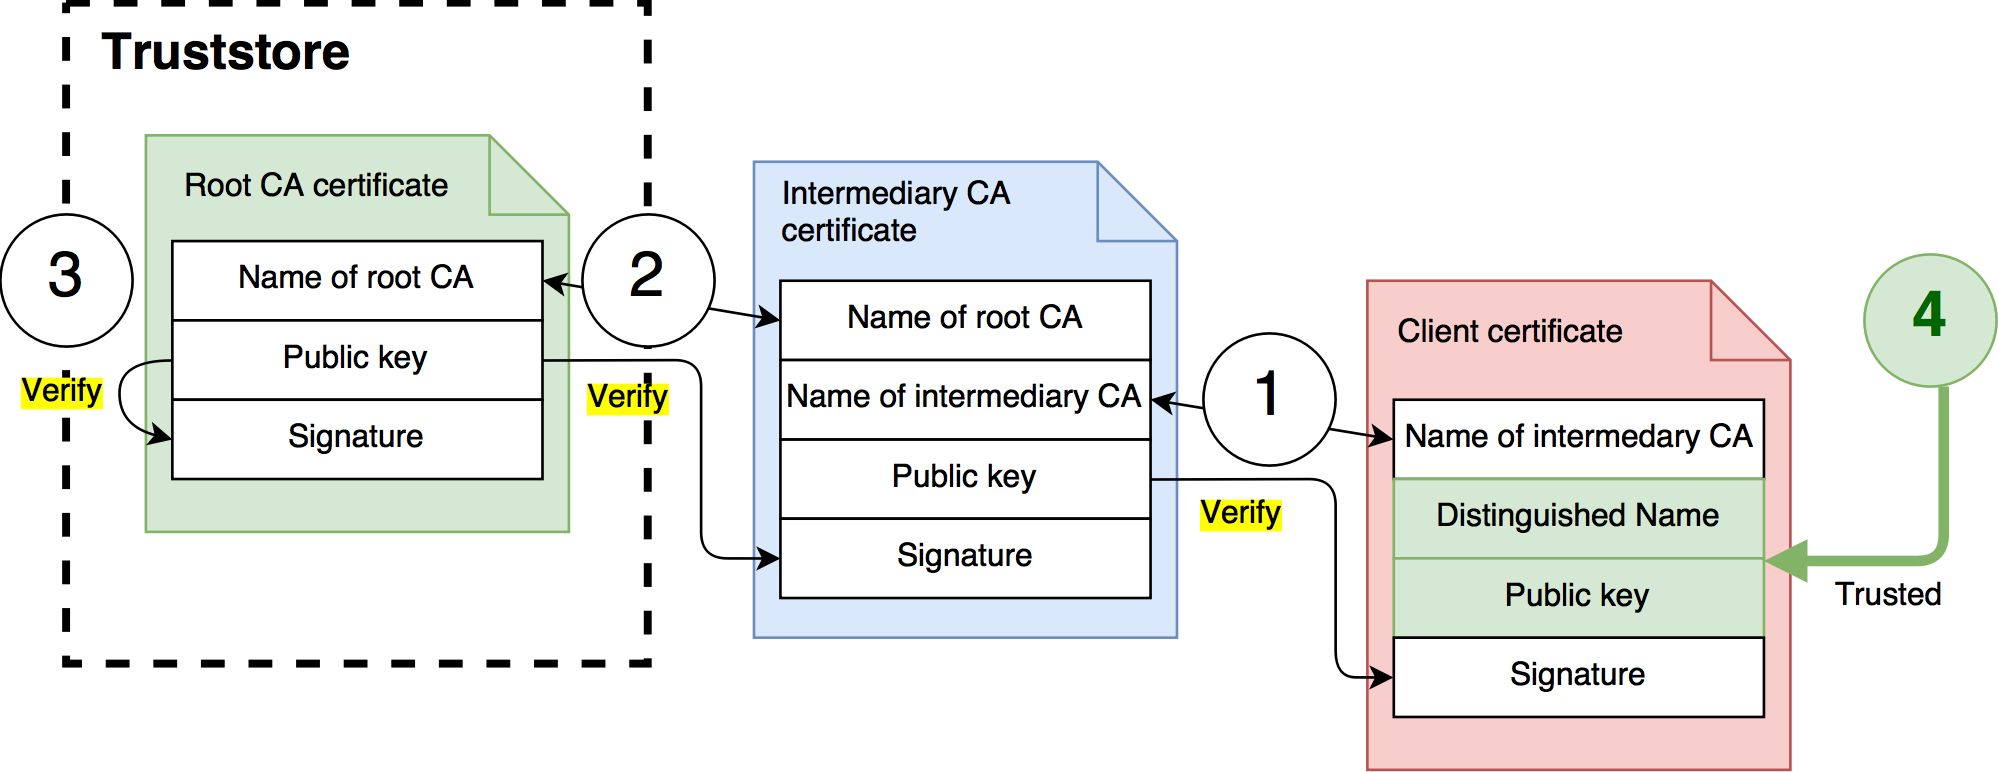
\includegraphics[width=\textwidth]{figures/fig-chain}
    \caption{A certificate chain with three certificates consisting of a root certificate (green), an intermediary certificate (blue) and a leaf certificate (red). The public key for the Distinguished Name (DN) in the certificate is trusted \ding{4} if the signatures in the chain are valid. To validate the certificate chain, the client has to check the signature of the leaf certificate using the public key of the intermediary CA \ding{1}, and check the signature of the intermediary CA using the public key of the root CA \ding{2}. The root certificate is self-signed \ding{3}.}
    \label{fig:chain}
\end{figure*}

\subsection{X.509 Certificates}
The most common format for certificates is defined in the X.509 standard and certificates following this format are called \textit{X.509 certificates} \cite{Ford00}. The format is shown in \cref{fig:x509v3}. The fields of a certificate are:
\begin{itemize}
    \item \textbf{Certificate Serial Number} Uniquely identifies a certificate issued by the CA.
    \item \textbf{Signature Algorithm Identifier} Contains the name and parameters of the signature algorithm used by the CA to construct the CA signature.
    \item \textbf{Issuer} The X.500 name of the certificate authority who has signed the certificate.
    \item \textbf{Validity period} Contains a start and expiry date which defines the period where the certificate should be considered valid.
    \item \textbf{Subject} The \emph{distinguished name (DN)} of the entity who owns the private key corresponding to the public key in the certificate.
    \item \textbf{Public key information} Contains the public key of the subject together with the algorithm and parameters used to construct the key.
    \item \textbf{Extensions} Added in X.509 version 3 and contains a list of certificate extensions.
\end{itemize} 

\begin{figure*}
    \centering
    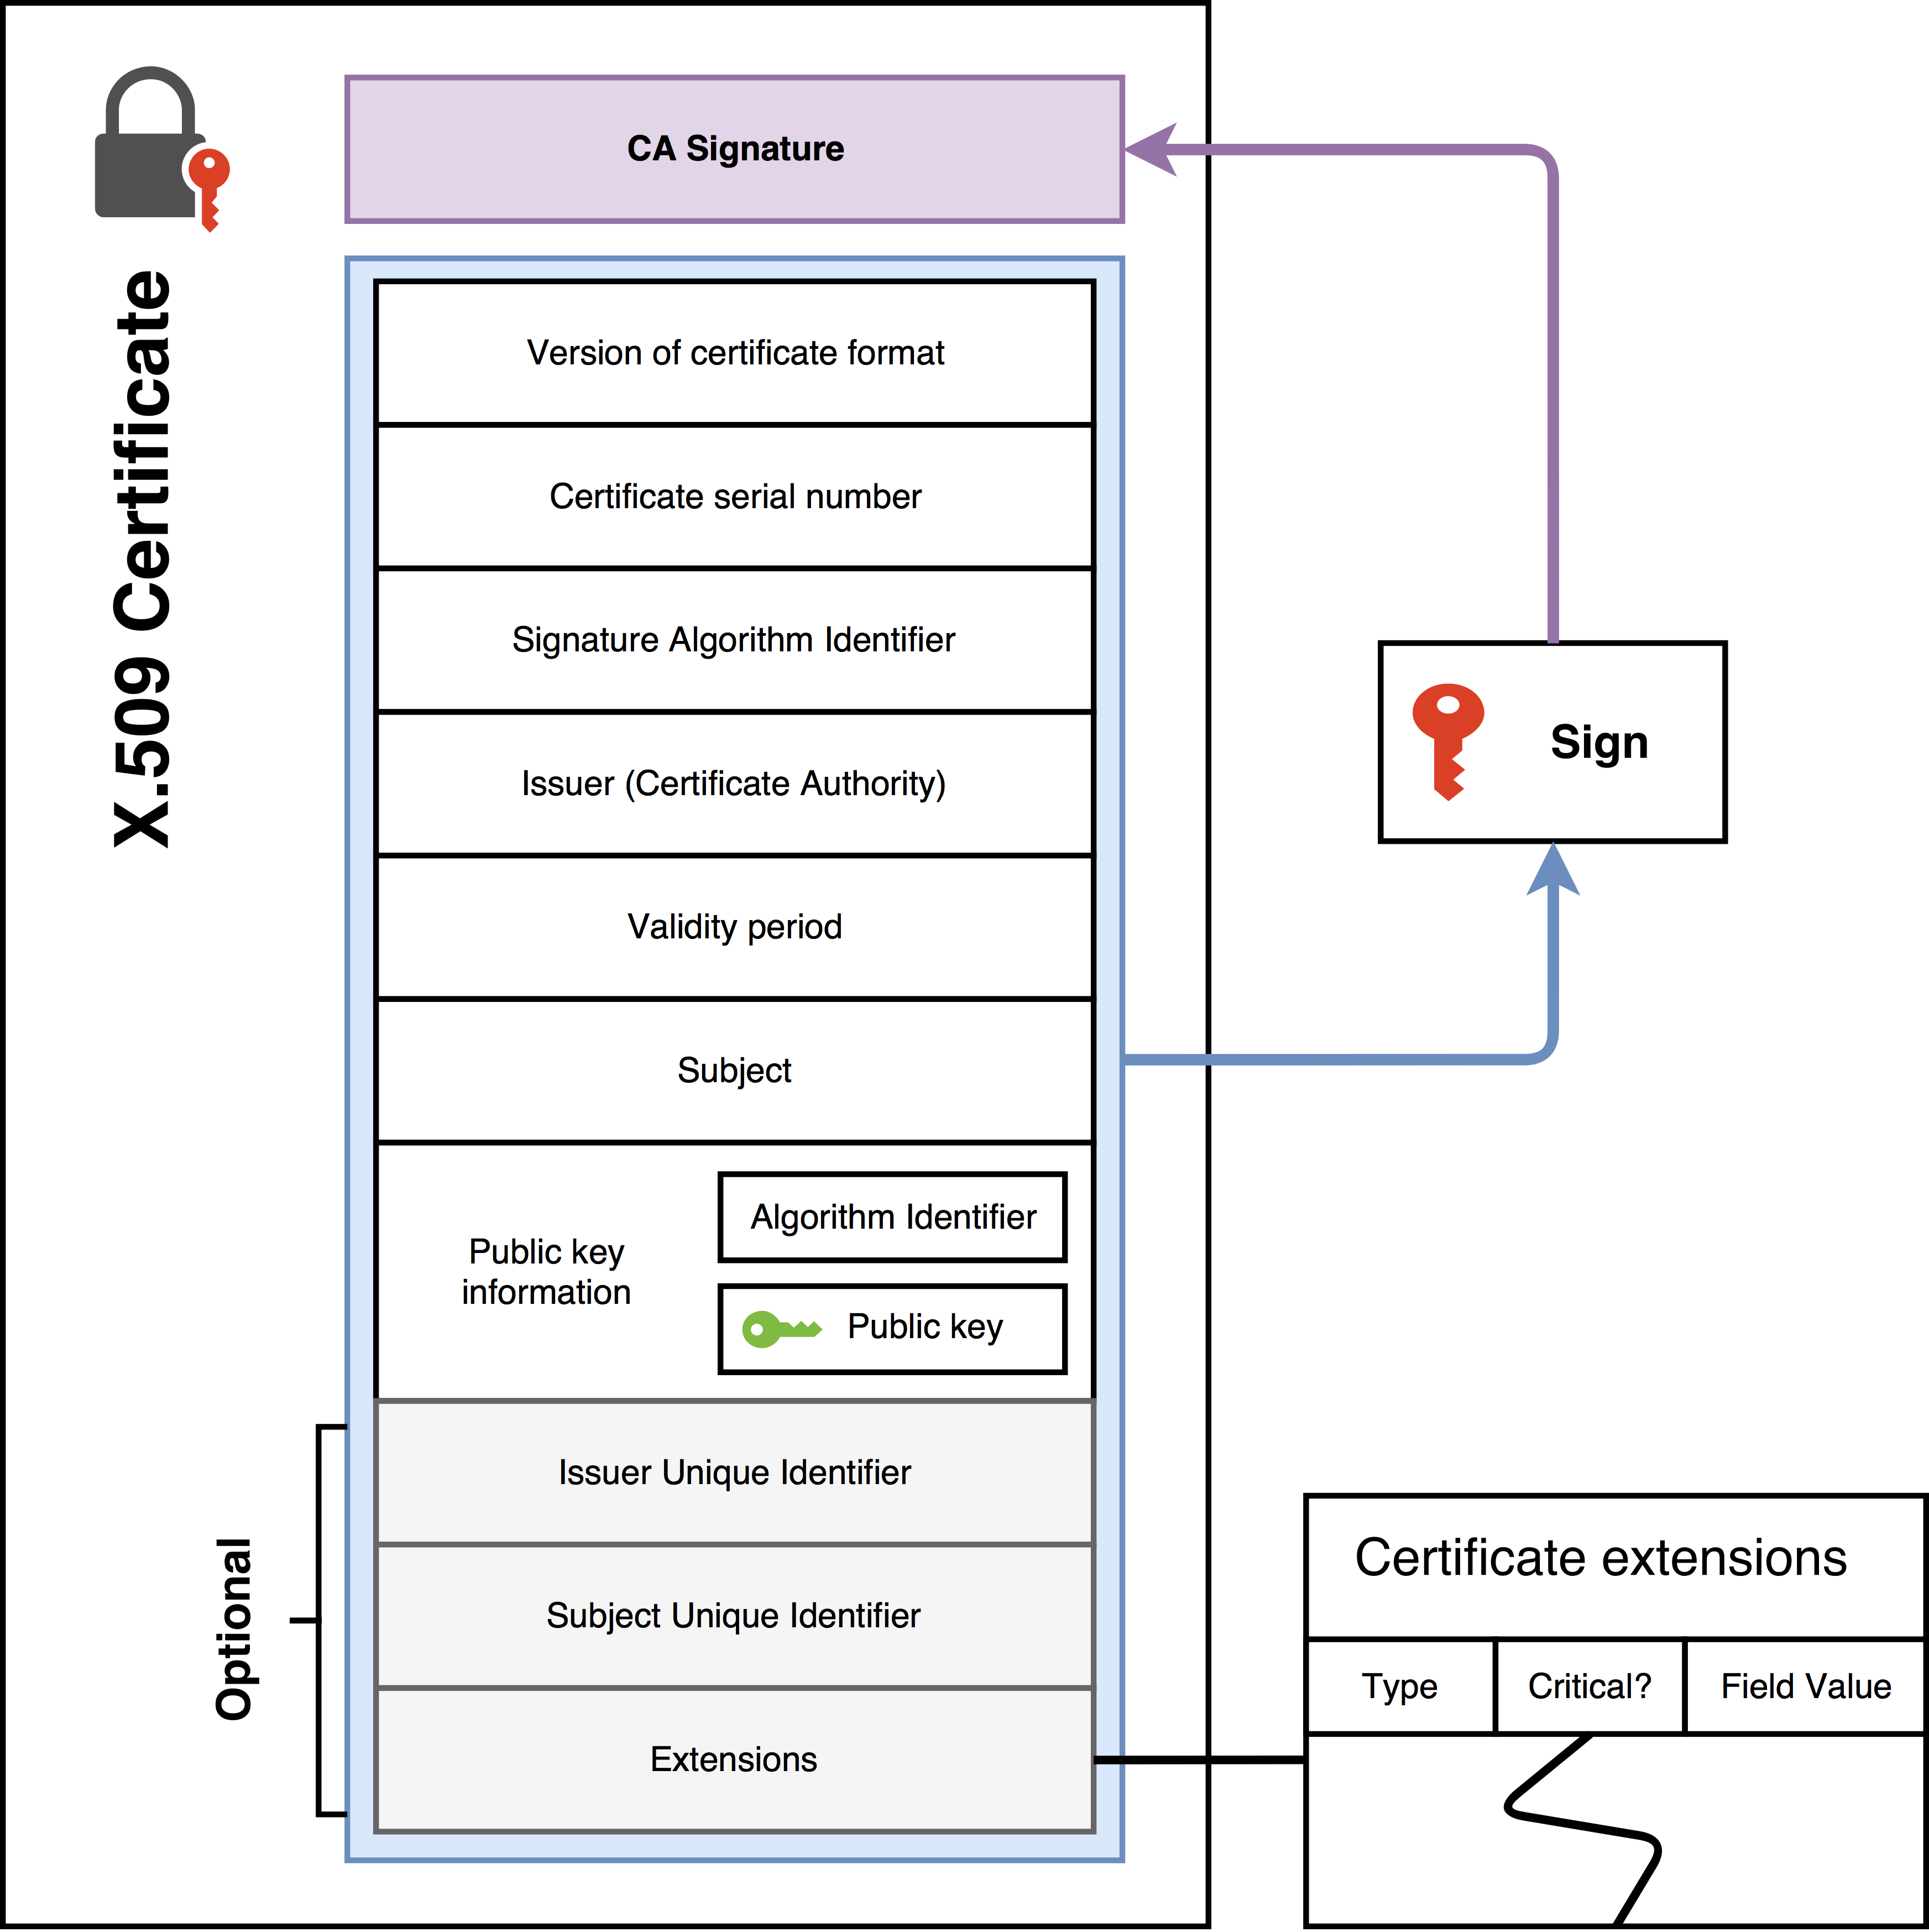
\includegraphics[width=\textwidth]{figures/x509v3}
    \caption{An image depicting version 3 of the X.509 certificate format. The public key information is trusted for the specified subject (certificate holder) if the CA signature is valid under the public key belonging to the issuer specified in the certificate, the certificate is presented within the specified validity period, and certificate has not been revoked.}
    \label{fig:x509v3}
\end{figure*}

For the purpose of this thesis, we are mostly be interested in certificate extensions which allow us to add additional functionality to a certificate. A certificate extension contains three fields: the type field, a critical bit, and a value field. The type field tells software, processing the certificate, what kind of certificate extension it is. The critical bit (if set) tells clients to reject the certificate, if support for the particular certificate extension is not yet implemented, and the value field contains the actual data of the certificate extension. There are currently 14 standardised certificate extensions, among them the basic constraints extension which allows a certificate to be used as a CA certificate \cite{Viega02}. There is no official limit on the size of a certificate extension, although Windows imposes a 4 KB limit on the field value, due to its CA database schema definition \cite{Stephens11}. A CA typically does not sign off on certificate extensions it does not understand, which means that any new certificate extensions must be implemented in the CA software.

\section{Pinning and Certificate Transparency}
In this section we look at two mechanisms for improving identity retention in the X.509 PKI and make it easier to detect fraudulent or misissued certificates.

\subsection{Public Key Pinning}
While the purpose of the certificate is to bind a public key to a name, if an adversary succeeds in issuing a fraudulent certificate to themselves with their own key, they could mount a man-in-the-middle attack and decrypt the traffic en route before reencrypting and forwarding the traffic to the victim. To prevent this from happening, a client could remember the key which was used the last time it connected and terminate the connection if the key suddenly changes. This is the idea behind public key pinning, a mechanism implemented in all major web browsers, used to enforce reuse of the same keypair for a specific domain. A server with pinning enabled sends $\mathsf{SHA2}$ hashes of its public keys (pins) in a specially crafted HTTP header, after a secure connection has been established. The pins are cached the first time a site is visited, and stored for the period of time specified in by the $\mathsf{max-age}$ header value. The next time the site is visited, the browser expects one of the pins to match one of the public keys in the certificate chain.

According to the specification, two keys must be pinned for security in case the first key gets lost. If both keys are lost, clients are no longer able to connect \cite{RFC7469}. It is possible to pin either the public key of the certificate authority, or the public key of the server certificate. Pinning the public key of the server certificate is safer, in the sense that it protects against certificate misissuance, but its presumably easier to accidentally lose the private key of the server certificate.

Public key pinning is a powerful weapon against a man-in-the-middle attack if implemented correctly. However, it has not gained much popularity. In a survey by Netcraft from 2016 \cite{Netcraft16} only 0.09\% of all websites had public key pinning enabled and one third of those websites deployed it incorrectly. One reason for why websites have been shy to adopt public key pinning might be that it can backfire if the server keys gets compromised. Since public key pinning does not offer any key recovery mechanisms apart from a backup key, it is almost impossible to recover from such a situation. Pinning the key of the certificate authority avoids this problem, but makes it harder to migrate from one CA to another and does not prevent misissuance for this CA. Public key pinning would also be unpractical in an environment where there are multiple servers, each with its own certificate and keypair, operating behind a load balancer serving requests for a single domain.

\subsection{Certificate Transparency}
The CA was previously the only entity who knew which certificates it had issued, which made it difficult to detect fraudulent certificates. Google's Certificate Transparency (CT) project \cite{RFC6962} tries to address this problem by providing publicly auditable, append-only logs, called \emph{Certificate Transparency logs (CT logs)} which contain certificates issued by a particular set of CAs. Third parties, called monitors and auditors, are making sure new certificates are appended to the log correctly, no certificates are being removed, and that logs are consistent. If a fraudulent certificate is detected, it can be reported by a monitor and revoked by the CA. 

The logs are structured as Merkle trees, described in \cref{merkle-tree}. The use of Merkle trees allows log operators to provide a succinct proof that a particular certificate is present in the log, called an audit proof, and that a log has been correctly updated with a new set of certificates, called a consistency proof.

The URL of the CT log is publicly advertised and anyone can interact with the log server through a REST API. When the CA posts a new certificate to the log, the log operator responds with a \emph{Signed Certificate Timestamp (SCT)}, which is a promise from the log operator to include the certificate before the time indicated in the SCT. The SCT itself is bundled with the certificate as a proof that the certificate has been submitted to a CT log. This is done either by requesting the SCT from the CA over OCSP using an OCSP extension, and then stapling this response with the certificate during the TLS handshake, or alternatively, the CA could include the SCT in the certificate itself, using an X.509 v3 certificate extension. Another option is to let the domain owner submit the certificate to the CT log, and then provide the SCT through a TLS extension during the TLS handshake.

Although CT makes it easier to find fraudulent certificates, it does not prevent fraudulent certificates from being issued in the first place. Domain owners are typically responsible for auditing and monitoring the logs themselves, which they are forced to do since there is no incentive structure in place for monitors to detect and report certificates for domains they do not own. There are also no procedures in place for automatically reporting fraudulent certificates, and it can take up to 24 hours before a certificate appears in the log. Domain owners relying on CT need to trust the log operator, and the log operator is typically decided by the issuer. 

\section{Blockchains}
A blockchain is an append-only public ledger replicated among all nodes in a large P2P-network, originally designed to store financial transactions for the Bitcoin cryptocurrency. The design of the Bitcoin blockchain was proposed by a pseudonym named Satoshi Nakamoto in 2009 \cite{Nakamoto08}, and since then several blockchains designed for different purposes have emerged. The blockchain offers consensus among entities in a decentralised network, effectively solving the problem of \emph{double spending} explained in \cref{blockchain-sec}. Physical money, such as bank notes, cannot be spent twice since they can only be in one place at a time. With the introduction of digital money in the form of credit cards, the double spending problem was solved by a clearing house, a central authority which approves transactions and keeps track of the balances for each account. Blockchains solves the double spending problem for digital money without a central authority. Instead, the central authority is replaced by an open, dynamic and decentralised P2P-network, where each node in the network keeps its own copy of the blockchain. Transactions are broadcast on this network and recorded on the blockchain, which can be thought of as a digital billboard, used by each participating party, to independently verify that a person has coverage for their expenditures. Due to the way blocks are added to the blockchain, once a block has been added it cannot easily be removed, hence it is hard to revert or change a transaction after it has been sent to the network.

A blockchain, in its original design, is a ledger which consists of blocks, each block contains a block header and a list of transactions. The list of transactions is linked to the block header through the root hash of a Merkle tree with the transactions as leaves. Each block header also contains a hash of the previous block, which links blocks to its predecessor in an ever-growing chain. Transactions are packaged and included in a block which is appended to the chain by a node in the network selected according to a \emph{consensus algorithm}. When a new block is created it is broadcast over the network, and participating nodes update their own local copy of the blockchain with the new block. Transactions are confirmed by consecutive blocks being appended, and a \emph{fork} may be created if two blocks are added at approximately the same time. How to resolve a fork is determined by the underlying consensus algorithm.

More generally, a blockchain provides a practical solution to the \emph{Byzantine Generals' Problem} \cite{Lamport82} where a set of decision makers try to a agree on a course of action through message-passing over an unreliable medium. More informally, a blockchain can be used to establish what ``truth'' is, which in the context of a PKI is to agree on a mapping between keys and their owners.

\subsection{Financial Transactions on a Blockchain}
\label{blockchain-transactions}
Bitcoin features a sequential transaction model which is used to transfer money between users in the system. Each transaction contains of a list of inputs $\mathbb{I}$, and a list of outputs $\mathbb{O}$. An output $o \in \mathbb{O}$ consists of an amount $|o|$ of coins bundled with a locking script $\sigma_{L}$ which puts an encumbrance on the output which has to be fulfilled in order to spend it. The most common encumbrance is to present a public key and signature with the corresponding private key, referred by hash in the locking script, which is called a \emph{Pay to Public Key Hash (P2PKH) transaction} depicted in \cref{fig:bitcoin-payment}. An input $i \in \mathbb{I}$ consists of a reference to an output, and an unlocking script $\sigma_{U}$ which fulfills the encumbrance defined in the referred locking script, more formally $\sigma_{L}(\sigma_{U}) = \mathsf{TRUE}$. The difference between the sum of coins in the input and the sum of coins in the output $\sum_{i \in \mathbb{I}}{|i|}-\sum_{o \in \mathbb{O}}{|o|}$, is indirectly interpreted as a \emph{transaction fee} collected by the miner who includes the transaction into the blockchain. An output is considered spent if it has been referred by a valid input a subsequent transaction. A node who keeps track of all transactions on the blockchain maintains a set of outputs which has not been spent yet, called \emph{Unspent Transaction Outputs (UTXO)}, determining the distribution of money in the system \cite{Antonopoulos14}.

Amounts for inputs and outputs are specified in \textit{satoshi}, the smallest unit of money which can be transferred in the system. Locking and unlocking scripts are typically written in a special-purpose scripting language which only supports the operations needed to perform a transaction. In Bitcoin, this scripting language is called \textit{Script}, a Forth-like reverse polish notation stack-based execution language. Script has two desirable properties which makes it suitable as a scripting language for programmable money. Firstly, it is a very simple language which requires little resources to execute, and cannot get stuck in for example an infinite loop or otherwise act maliciously, possibly crashing the host computer. As a consequence, Script is not Turing complete and does not have the expressiveness of a full programming language. Secondly, Script offers stateless verification, meaning all the information needed to execute the script is in the script itself. This guarantees that the execution of a script is consistent among all nodes participating in the network \cite{Antonopoulos14}.

\subsection{Simple Payment Verification}
\label{spv-client}
Simple Payment Verification (SPV) is a method used to verify transactions without storing the whole blockchain. Clients relying on SPV are called \emph{SPV clients} or \emph{thin clients}. SPV is important for low-powered devices with limited processing and storage capabilities such as smartphones and laptops. 
A thin client typically only downloads and verifies the block headers, which are small in size and can be verified quickly. Block headers belonging to the longest chain are assumed to be hard to fabricate since they require Proof of Work, and are used as a trusted source of information, which is used to verify transactions. A thin client verifies the existence of a set of transactions $\mathbb{T}$, by submitting a \emph{Bloom filter} containing $\mathbb{T}$ to the network. The network answers with a set of transactions matching the Bloom filter, together with a set of Merkle proofs, which proves that a transaction was included in a specific block \cite{BIP0037, Antonopoulos14}. 

Since a Merkle proof is as hard to fabricate as creating a collision in the underlying hash function \cite{Coronado05}, a thin client cannot be fooled into believing a transaction has been confirmed by the network, when in fact it has not. However, thin clients do have two other significant drawbacks in terms of security: Firstly, it is possible to hide the existence of a transaction, which has been confirmed by the network in a subsequent block. The only way for a thin client to counteract this, is to request Merkle proofs from many different nodes, hoping they are not all malicious. This assumption may prove problematic if a large portion of the network consists of malicious nodes, which might be the case if the network falls victim for a \emph{sybil attack}. Secondly, since thin clients do not verify transaction history, they cannot detect a double spend in the past. Thin clients do instead rely on block leaders to not confirm blocks with conflicting transactions.

\begin{figure*}
    \centering
    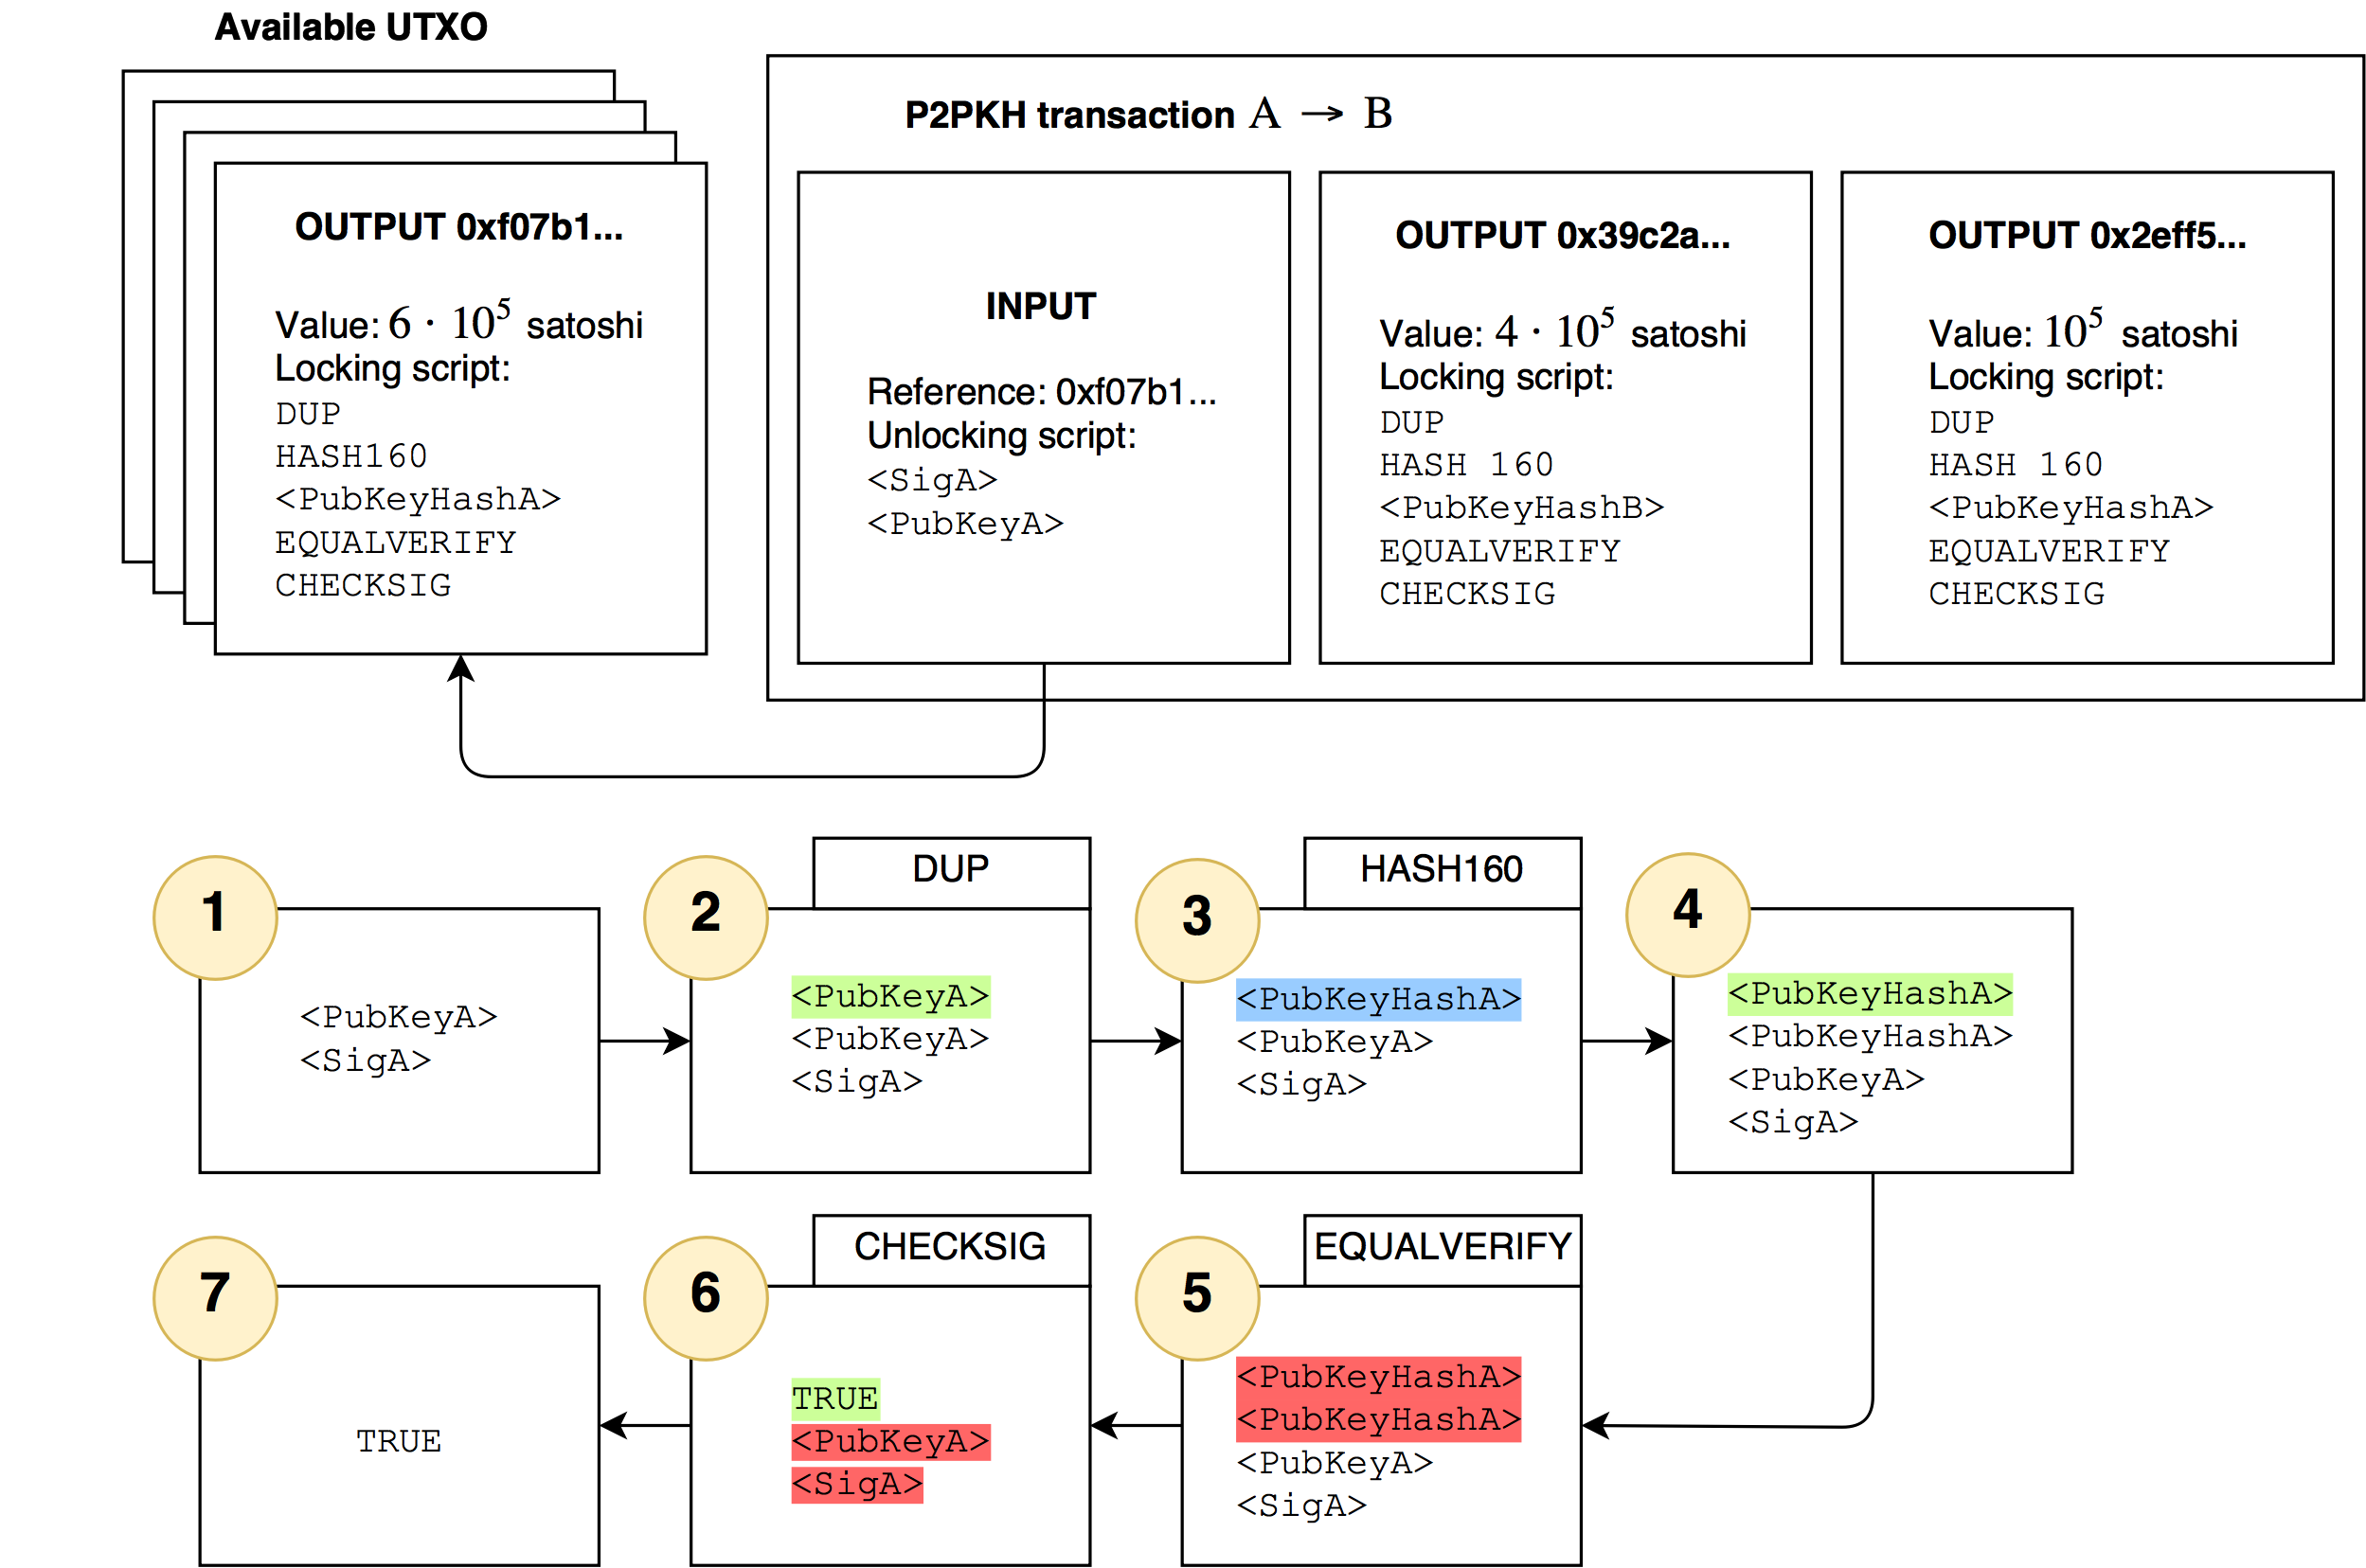
\includegraphics[width=\textwidth]{figures/bitcoin-payment}
    \caption[skip=50pt]{A Pay to Public Key Hash transaction from an address $A$ to another address $B$ in Bitcoin, created from one Unspent Transaction Input with hash $\mathsf{0xf07b1}\ldots$ containing a total of $5 \cdot 10^5$ satoshi locked with $A's$ private key. The transaction transfers $4 \cdot 10^5$ satoshi to $B$ (through the $\mathsf{0x39c2a}\ldots$ output), keeping $10^5$ satoshi as change (through the $\mathsf{0x2eff5}\ldots$ output) and giving another $10^5$ to the miner who processes the transaction and includes it into their block. The validation of the transaction can be checked by running the locking script of the $\mathsf{0xf07b1}\ldots$ transaction with the output of the unlocking script in the input transaction. Execution begins with the signature and the public key of the unlocking script being pushed onto the stack. The $\mathsf{DUP}$ instruction duplicates the element on the top of the stack, and the $\mathsf{HASH160}$ instruction replaces the value on top of the stack with its hash. Next, the public key hash of the locking script is pushed on the stack and the $\mathsf{EQUALVERIFY}$ instruction pops the two elements on top of the stack if they are equal. Finally $\mathsf{CHECKSIG}$ pops the public key and the signature from the stack and pushes $\mathsf{TRUE}$ if the signature is correct.}
    \label{fig:bitcoin-payment}
\end{figure*}

\subsection{Proof of Work}
\label{pow}
Proof of Work, also called \textit{Nakamoto consensus} is the consensus algorithm which is used by a number of blockchains including Bitcoin, Lightcoin and Ethereum. In Proof of Work, there are machines working on solving a time puzzle, called \emph{miners}. The next \emph{block leader} becomes the machine who first solves the puzzle.

The puzzle is constructed in such a way that it is hard to solve but easy to verify, which in cryptography is called a \emph{trapdoor function}. Bitcoin uses a variant of hashcash, which originally was intended to be used to limit spam in email systems. In Bitcoin, the puzzle to solve is to find a $\mathsf{SHA2}$ hash value $\mathsf{SHA2}^2(\text{block header})$ such that $\mathsf{SHA2}^2(\text{block header}) < 2^{(n - k)}$, where $n = 256$ is the number of output bits in the $\mathsf{SHA2}$ hash function and $k$ is a difficulty factor, collectively determined by the nodes in the network every 2016 blocks, such that on average a new block in appended to the blockchain every 10 minutes \cite{Antonopoulos14}.

The \emph{longest chain} in Bitcoin's Proof of Work is considered to be the blockchain with the most accumulated difficulty $\sum{k}$. When a fork is created, a copy of both chains are kept, until the fork is resolved which typically happens when the next block is added, making one of the chains longer than the other \cite{Antonopoulos14}.

Miners are incentivised to add new blocks to the blockchain by collecting transaction costs, and by the \emph{block reward} which is paid to the address found in the first transaction in the block, called the \emph{coinbase transaction}. The coinbase transaction does not transfer money from anyone, but creates new money which can be spent after the block has enough confirmations \cite{Antonopoulos14}.

Since consensus based on Proof of Work requires miners to buy expensive hardware and consume large amount of electricity, adding a new block to the blockchain becomes economically expensive. Estimates shows a net cost between \$6 and \$10 per transaction \cite{Davarpanah15, Croman16}, while the actual transaction costs paid today are significantly lower. Bitcoin users are currently shielded against these costs through the block reward which pays for the electricity consumed by the miners. But since this block reward is halved every 210000 blocks, there is a risk for transaction fees to going up over time, or miners dropping out when mining no longer becomes profitable \cite{Kaskaloglu14}.

Another problem with Proof of Work is its environmental impact. A study from 2014 estimates the electricity consumption of the whole Bitcoin network to be on par with Ireland \cite{ODwyer14}. Furthermore, since chip manufacturers are in a constant ``electronics arms race'' competing in producing cheaper and more resource efficient ASICs, it forces miners to constantly upgrade and replace their equipment to stay competitive. This results in a large amount of electronic waste. Highly specialised mining rigs such as ASICs used for Bitcoin mining, are useless for anything else than computing SHA2 hashes and has little to none second-hand value. Some \textit{altcoins} tries to combine or replace seemingly useless hash computations with something more meaningful. As an example, Gridcoin combines the hash function scrypt with participation in the BOINC grid computing network, which harnesses the computing resources of its participants for scientific research, and Curecoin combines SHA2 with protein-folding research through the Folding@Home project \cite{Antonopoulos14}. 

New blockchains based on Proof of Work would require a large amount of hashing power to be secure. This would either require a huge investment in equipment or persuading existing miners to join the network. The latter could be addressed with \emph{merged mining} where a miner is able to mine on two chains at the same time, without splitting their hashing power in two. The idea is to piggyback an \emph{auxiliary chain} onto another \textit{parent chain} (such as the Bitcoin blockchain). A miner doing merged mining would create a block for the auxiliary chain, hash the block header and include this hash in the coinbase transaction of the parent chain. A block header for the auxiliary chain contains some additional data, such as the coinbase transaction of the parent chain, and a Merkle proof which proves that the coinbase transaction is in the parent block. This information can then be used to validate the block in the auxiliary chain using the block headers of the parent chain. There are financial incentives for miners to do merged mining since they can get rewards from mining on the auxiliary chain without additional expenses. However, merged mining comes with a couple of caveats: Firstly, a large mining pool which suddenly decides to start to merge mine another blockchain can end up controlling a large part of the chain's hashing power. Secondly, merged mining requires a hard fork\footnote{A hard fork is a software update which is not backward compatible with previous versions of the software.}. While this might be a feature easy to add, it might be harder to remove at a later stage if needed, since the user base is more spread out and not likely to abandon the additional revenue stream from the auxiliary blockchain. Thirdly, due to size constraints on the coinbase transaction, there is a limitation on the number of auxiliary chains which can be merged mined at the same time \cite{BitcoinWiki0220}.

\subsection{Proof of Stake}
Proof of Stake is another  way of reaching consensus within a decentralised network. Instead of utilising miners, Proof of Stake based systems selects a block leader based on how many coins they put at stake. The idea is that, someone who is rich would have incentive to be benevolent, since any malicious behaviour is undermining their own wealth. To take control over the system, one needs to acquire a large portion of the coins in circulation, which might be more expensive than buying large amounts of mining equipment. Proof of Stake is more cost effective than Proof of Work since it does not rely on miners consuming large amount of electricity.

The first cryptocurrency based on Proof of Stake was Peercoin \cite{King12} which uses a hybrid between Proof of Work and Proof of Stake. Peercoin introduced the notion of \emph{coinage} which is the time a coin has been idle. A coin's coinage is being consumed and set to zero when the coin is put at stake to generate a block or when transferred to another wallet. The longest chain is then considered to be the chain with the most coinage consumed, and forks are resolved in the same way as in Bitcoin's Proof of Work. To create a new block, one needs to control a set $\mathbb{S}$ of unspent coins which have been idle for a minimum time period, called \emph{minimum stake age}, and find a block header fulfilling the Peercoin mining formula:
\begin{equation}
H(\text{block header}) \le k \sum_{\mathsf{coin} \in \mathbb{S}}{\mathsf{age}(\mathsf{coin})}    
\end{equation}
where $k$ is a difficulty factor adjusted by the network after every block and $\mathsf{age}(\mathsf{coin})$ is the coinage of a coin \cite{Davarpanah15}. The first transaction in the block, called \emph{coinstake transaction} (the equivalence to Bitcoin's coinbase transaction), pays the miner the coins at stake back to himself which effectively destroys some (or all) of their coinage. In order to provide incentive for stakeholders to stake money, they are awarded with 1\% interest rate per coin year consumed.

Proof of Activity \cite{Bentov14} tries to extend the Proof of Work scheme used in Bitcoin through a Proof of Stake mechanism where a miner creates an ``empty'' block with no transactions meeting the current Proof of Work difficulty target. A list of $N$ stakeholders is derived from this block header through a process called \emph{follow-the-satoshi}. The first $N - 1$ stakeholders signs the block with their private key and the last stakeholder finalises the block by collecting a list of transactions, signing the result and broadcasting it to the network.

Follow-the-satoshi is a deterministic, psuedo-random process which can be seen as a lottery, where the winner of the lottery is the owner of a satoshi chosen uniformly at random using a \emph{cryptographically secure psuedo-random number generator (CSPRNG)} seeded with information found on the blockchain. The seed can be derived from a secure multiparty computation, for example by allowing each block leader to put some randomness in the block header of their block.

One such approach is Ouroboros \cite{Kiayias16} which is a provably secure Proof of Stake model based on a commitment scheme. In Ouroboros, time is divided into epochs, and an epoch is divided into timeslots. The CSPRNG is reseeded after every epoch, and used to derive a set of lucky stakeholders which are allowed to generate a new block during their designated timeslot. To generate the randomness, Ouroboros features a coin flipping protocol with guaranteed output delivery. Stakeholders participating in the coin tossing protocol commits to a value using a commitment scheme. Shares of the committed value are distributed to the other entities using \emph{Verifiable Secret Sharing (VSS)}. When all stakeholders have committed and received their shares, they can reveal the committed value. The revealed values are then mixed together and used to derive new stakeholders for the next epoch using follow-the-satoshi. If a malicious stakeholder refuses to reveal their commitment, the other stakeholders can cooperate to reconstruct the committed value using the shares they received when the commitment was made. The longest chain is defined as the chain with the most blocks, and accidental forks are not possible since follow-the-satoshi uniquely determines the next stakeholder allowed to generate a new block.

\subsection{Blockchain Security}
\label{blockchain-sec}
Blockchains used for financial transactions are designed to mitigate \emph{double spending attacks} where an adversary is trying to spend the same coin twice, for example by buying different goods using the same coin. To succeed with this attack, an adversary $A$ must create two conflicting transactions by forking the main chain and then make the network accept the fork. Suppose we have a merchant $M$ who waits for $c$ confirmations before shipping a product. After the product has been shipped, the blockchain looks as follows: $B_1, B_2\ldots B_i, B_{i+1}, B_{i+2}\ldots B_{i+c}$ where block $B_i$ contains a transaction which transfers money from $A$ to $M$. Assuming the computational difficulty $k$ is equal for all blocks, an adversary who wants to double spend this money, must (in secret) create a fork $B_1, B_2\ldots B_{i-1}, B'_{i}, B'_{i+1}\ldots B'_{i+c'}$ where $c' > c$ and any of the blocks $B'_{i}, B'_{i+1}, B'_{i+c'}$ contains a conflicting transaction. When this fork is broadcast to the network, it is accepted as the new main chain, overwriting all transactions in the last $c$ blocks. This scenario is depicted in \cref{fig:double-spend}.

\begin{figure*}[ht!]
    \centering
    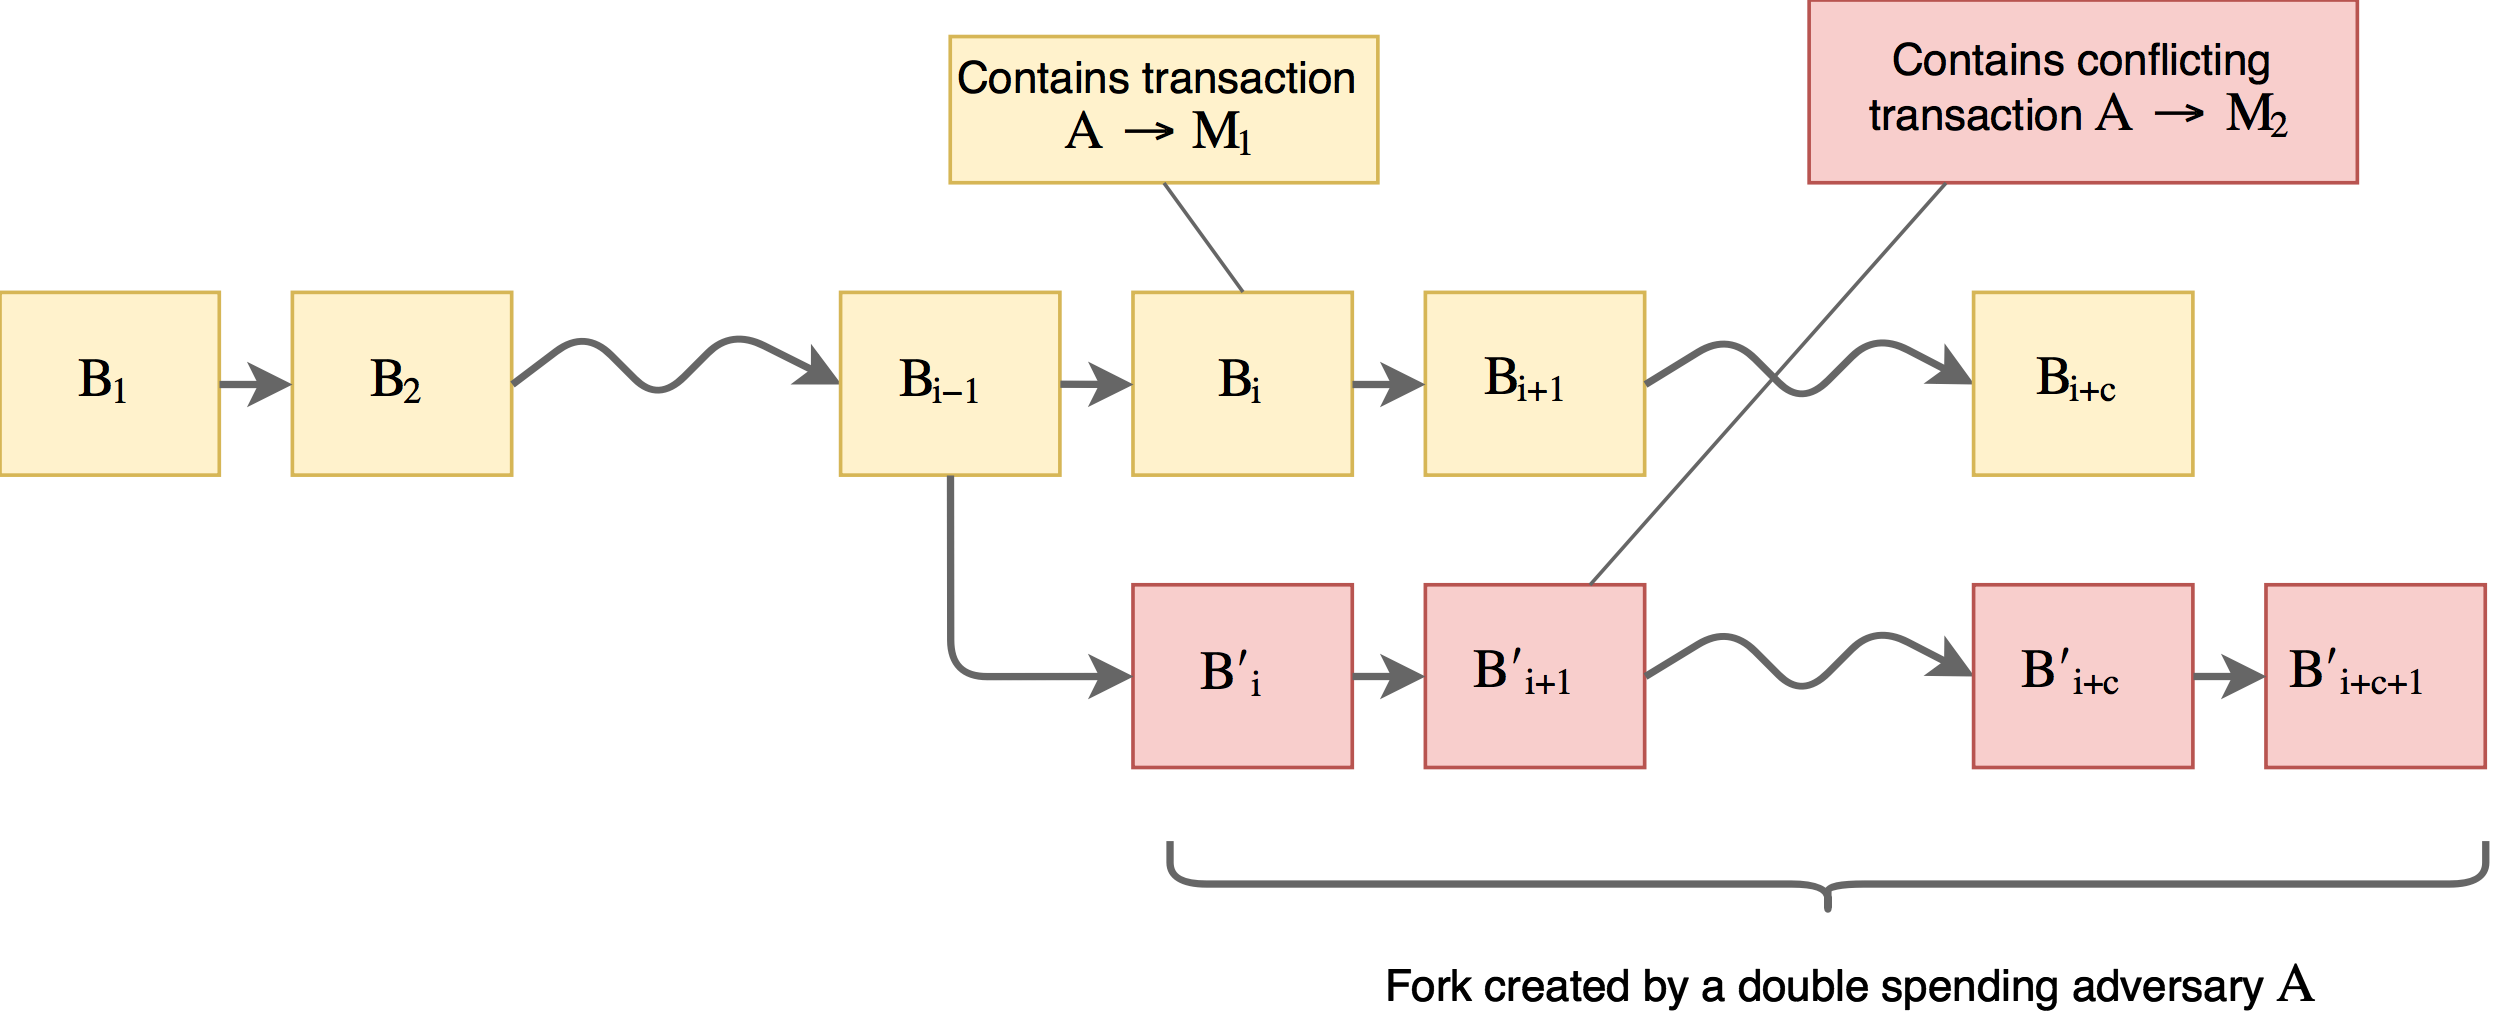
\includegraphics[width=\textwidth]{figures/double-spend}
    \caption{A double spending attack against a merchant $M_1$ waiting for $c$ confirmations. A double spending adversary $A$ creates a fork $B_1, B_2\ldots B_{i-1}, B'_{i}, B'_{i+1}\ldots B'_{i+c+1}$ with larger accumulated difficulty, which is accepted as the new main chain by the network, overwriting the transaction $A \rightarrow M_1$ with the conflicting transaction $A \rightarrow M_2$.}
    \label{fig:double-spend}
\end{figure*}

Bitcoin and other cryptocurrencies based on Proof of Work protects against this kind of attack by making it computationally expensive to produce a new block. This means that an adversary $A$ have to spend a lot of money on electricity and equipment to perform a double spend, and if a merchant waits for enough confirmations, it becomes more expensive to create a fork and double spend the money than to simply spend the money twice. We say that Bitcoin is \emph{economically secure}.

With this in mind, a common argument against Bitcoin and other blockchains based on Proof of Work, is that an adversary can buy themselves power by purchasing mining rigs. An adversary, or a colluding group of adversaries, controlling a majority of the hashing power, can then execute a 51\%-attack, where an adversary can deny, or even double spend some transactions. However, even an adversary with a majority of the mining power will be unable to revert transactions with enough confirmations, since the probability of an adversary overwriting a transaction within a block, drops exponentially with the number of confirmations \cite{Nakamoto08}. Any blockchain with an open consensus process might potentially be a victim for a 51\%-attack, since there is no authority which can deny participation.

A perhaps more serious threat against blockchains based on Proof of Work, is selfish mining \cite{Eyal13} which dictates a strategy for a colluding group of adversaries, controlling at least 25\% of the mining power in the network, to mine on their own ``private blockchain'' and selectively publish blocks to decrease the profits for the honest miners. Thus, honest miners are incentivised to join the group of colluding adversaries, which at some point might grow large enough to mount a 51\% attack.

Another type of attack is a \emph{denial of service attack} where an adversary tries to disrupt the operation of the network by sending spam transactions with low transaction fees, called \emph{dust}. We refer the reader to \cite{Baqer16} for more information.

Blockchains based on Proof of Stake, such as Peercoin, raises some additional security concerns which has to be addressed. Firstly, an adversary could build on its own fork without additional mining equipment, which can undermine the ability for the network to reach consensus. Secondly, an adversary could try to use the private keys acquired from old wallets to rewrite the transaction history. Such wallets could presumably be bought cheaply from people who no longer have any stake in the system. Thirdly, an attacker could try to use their computing power to grind through a lot of different block headers until they find a block header which improves the performance of their stakes, called \emph{stake grinding}. These issues are investigated in more detail in \cite{Davarpanah15}. To provide an additional security guarantee against these kind of attacks, the Peercoin blockchain offers regular \emph{checkpoints}, where the Peercoin creator Sunny King digitally signs the blockchain \cite{King12}.

\subsection{Scalability Concerns}
\label{scalability-concerns}
A system which intends to be global and process a large amount of transactions needs to scale in order to function correctly. Unfortunately, most blockchains are quite inefficient in terms of transaction throughput and storage requirements. As an example, consider the Bitcoin blockchain, which is the most popular blockchain to date. It processes on average 1.57 transactions per second with a theoretical maximum throughput of 3.3 to 7 transactions per second \cite{Croman16}. This is about as many transactions per second, as processed by Let's Encrypt CA, which issued on average 4 certificates per second in December 2016 \cite{LetsEncrypt17}. Considering Let's Encrypt had a market share of 0.1\% during this time period \cite{W3Techs17} it is clear, that in order to use blockchains for a distributed PKI on a large scale, major improvements are needed. Furthermore, the Bitcoin blockchain had a total ledger size of about 96 GB as per Februari 2017, growing linearly over time at a rate of about 4 GB per month \cite{Blockchain17}. Although a node could prune the transactions after they have been buried under enough blocks and only store the UTXO permanently (which is about 1.6 GB in size \cite{Statoshi17}), a new node needs to download and validate all transactions before booting up. This process, called \emph{bootstrap time} takes about four days \cite{Croman16}, and increases with time as new blocks are appended to the blockchain.

\subsubsection{Transaction Throughput}
In a peer to peer setting, where all participating nodes are validating and broadcasting the transactions in the network, the number of transactions per second $|\mathbb{T}|$ which can be confirmed by the network is limited by the block size $B_s$ and the block interval $B_\Delta$ in seconds according to $|\mathbb{T}| = \frac{B_s}{B_\Delta \cdot \mu_t}$ where $\mu_t$ is the average transaction size for the block $B$. 

Thus, the only way to increase the throughput of the blockchain is to increase the block size, decrease the average transaction size or lower the block interval, and the block size is limited to the bandwidth of the individual nodes. In Bitcoin, an increase in block size or decrease in block interval increases the probability of a fork. Forks incur a security risk since it gives an opportunity to submit two conflicting transactions in two different blocks, which can lead to a double spend (see \cref{blockchain-sec}). Forks are also lowering the security of the blockchain, since the mining power is split in half, making it easier to attack the network.  Furthermore, storage and communication costs of the individual nodes goes up, which might lead to centralisation when smaller nodes cannot afford the equipment required to run a full node, and decide to drop out of the network. Forks can also lead to inefficiencies owing to transactions belonging to orphaned blocks being moved back into the \emph{mempool}. There have been discussions about an increase of the current 1 MB block size in Bitcoin \cite{BIP100, BIP101, BIP102, BIP103}, all requiring a hard fork of the Bitcoin software, but at the time of writing none of these proposals have taken effect.

\subsubsection{Bitcoin-NG}
The rate at which the Bitcoin network can confirm transactions is mostly due to Bitcoin's leader election rather than limited by the speed of the individual network links. Bitcoin's block leader is chosen by Proof of Work (as discussed in \cref{pow}) seemingly arbitrarily every 10 minutes. As a consequence, the network traffic in Bitcoin becomes rather bursty: A chunk of transactions move from the mempool to the blockchain only when a new block leader is elected, while the network remains almost idle the rest of the time. As a consequence, the link capacity of the network is not fully utilised, which reduces throughput. 

Bitcoin-NG \cite{Eyal15} tries to solve this problem by decoupling leader election with transaction serialisation. In Bitcoin-NG, there is one blockchain with two types of blocks, \emph{keyblocks} and \emph{microblocks}: A miner starts a new \emph{epoch} by generating a keyblock through the same Proof of Work mechanism as in Bitcoin. The keyblock contains a single coinbase transaction with the leader's public key. Once a leader has found a keyblock, they are eligible to process transactions, which are packed into microblocks and signed by the leader's private key. A microblock is valid when all transactions are valid, and the block is correctly signed by the key of the block leader as specified by the most recent keyblock. Microblocks require no Proof of Work and can be produced as fast as they can be propagated and processed by the block leader. As a consequence, the available bandwidth in the network is used more evenly which results in a higher throughput. Transactions can also be confirmed much faster, since they do not need to be cached in the mempool until a miner finds the next keyblock. 

A benefit of Bicoin-NG is that it shares the same, solid trust model as in Bitcoin. Transaction fees are split 40/60, that is 40\% of the fees are given to the current block leader, and the remaining 60\% procent are given to the next block leader. Some concerns regarding double spending has been raised: A malicious block leader could try to double spend within their epoch, by generating a fork of microblocks containing a conflicting transaction. To discourage such behavior, Bitcoin-NG features a \textit{poison transaction} which invalidates the block leaders revenue if a fork is detected. The poison transaction must be placed after the subsequent keyblock, but before the malicious block leader has spent their transaction, and can only be submitted once. Since all microblocks are signed by the block leader, one can provide a proof of malice by including the header of the first microblock in the fork. This information is put in the poison transaction together with an address which receives a 5\% compensation of the confiscated revenue.

\subsubsection{ByzCoin and the CoSi Protocol}
ByzCoin \cite{Kokoris16} combines a Practical Byzantine Fault Tolerance (PBFT) algorithm with Bitcoin's Proof of Work. Each microblock must be co-signed by a two-thirds supermajority of nodes in a consensus group before being appended to the blockchain. Hash power-proportionate consensus groups are formed after each keyblock, by taking the $N$ most recent block leaders and placing them in a tree with the current block leader as the root. Blocks are co-signed with Schnorr's signature scheme using the CoSi protocol. The CoSi protocol allows for efficient distribution and computation of signatures, by leveraging the ability to aggregate Schnorr signatures. We refer the reader to \cite{Syta16} for a detailed description of the CoSi protocol.

\subsubsection{Cryptonite}
Apart from throughput, one should also consider the size of the blockchain itself. The mini blockchain scheme \cite{Bruce14}, implemented in the Cryptonite cryptocurrency, addresses this problem by leveraging the possibility of completely pruning old transactions from the blockchain, and only keep the block headers, called a \textit{proof chain}. Since pruning makes it impossible to verify transaction history, the database of unspent coins is replaced with an \emph{account tree} and transactions becomes operations on this account tree. A drawback with Cryptonite is the lack of support for scripts, all operations on Cryptonite's account tree are similar to Bitcoin's P2PK transactions.

\chapter{Methodology}
\label{chap:method}
This chapter contains the design goals we attempt to achieve, explains our approach for solving the problem and defines the entities in our proposed PKI.

\section{Design Goals}
In choosing how to proceed, we need to consider the design goals we want to achieve.

\begin{itemize}
    \item \textbf{Identity retention} An identity should, to the furthest extent possible, only be able to be issued, changed or revoked after permission from the person or organisation owning the identity. The current PKI achieves this through strict vetting rules where a CA requires proof in form of paperwork, or physical presence of an employee acting on behalf of the organisation before a certificate is produced. These procedures occasionally fail, due to not being carried out properly or not at all, which can result in impersonation. We believe a stronger guarantee for identity retention of already existing identities can be enforced by public key cryptography, where new certificates need to be signed by the organisation's private key.
    \item \textbf{Expiration of old identities} There should be a mechanism where identities are renewed on a regular basis, and old identities are purged. This reduces storage requirements, since identities which are no longer active can be forgotten, and avoids ``locking up'' names in our naming system. 
    \item \textbf{Key recovery} If a private key not known to the CA is required to issue new certificates, what happens if this key is lost? In a naive setting, no new certificates would be able to be signed until the identity expires. To avoid such a situation, key recovery mechanisms are required where servers can specify backup keys which can be kept in cold storage or distributed to a trusted third party.
    \item \textbf{Transparency} Anyone should be able to connect and retrieve a ``global'' view of the all identities in the system, and being able to verify every transaction. This is important to be able to detect fraudulent behavior, without relying on a central authority.
    \item \textbf{Scalability} The system needs to scale in a reasonable way when more and more identities are registered. Namely, storage and bandwidth requirements should be met by consumer off-the-shelf hardware, and the system should be able to handle enough transactions to scale globally.
    \item \textbf{Backward compatible} Processes for issuance, revocation and verification of names and public keys should be compatible with the current PKI if possible.
    \item \textbf{Thin client support} The system should support thin clients, to permit certificate verification for low-powered devices such as smartphones.
\end{itemize}

\section{Our Approach}
Our approach is to assign a public key to each domain holder. The public keys are stored in a Merkle tree, whose root hash is stored in a block on the blockchain. Thin client support is achieved by the use of Merkle proofs, which can prove the existence of public key mapping without requiring a client to download the whole tree. To keep the system compatible with the current PKI, we use certificates as usual, but ensure these are cross-signed by the domain holder's private key. Key recovery mechanisms can be built into the system, by locking each public key in the tree with a Bitcoin script. To ensure the Merkle tree is updated properly, custom-built blockchain nodes are needed. Thus, a decision was made to build our own blockchain, which also avoids us the limitations in throughput, present in some of the public blockchains in use today. A custom Proof of Stake protocol is proposed which is based on a set of semi-trusted \emph{stakeholders} who take turns in adding blocks to the blockchain. 

\section{System Model}
The entities involved in our distributed PKI are clients and servers trying to establish secure connections among themselves, and a set of blockchain nodes operating a large P2P-network. Some of these blockchain nodes are stakeholders, and may be chosen to approve transactions sent to the network.

\begin{itemize}
    \item \textbf{Stakeholder} A semi-trusted entity such as a government, CA or browser vendor authorised to maintain the blockchain.
    \item \textbf{Blockchain CA} A CA approved by the stakeholders eligible to approve new transactions processed by the stakeholders.
    \item \textbf{Validator} A third party who monitors the blockchain network to ensure everyone follows the protocol.
    \item \textbf{Thin client} The client of an end-user (such as a web browser) with limited processing, storage and bandwidth abilities.
    \item \textbf{Domain owner} An owner of a DNS domain name, running a web service.
\end{itemize}

\section{Choice of signature scheme}
Unless otherwise specified, keys are assumed to be a point on a 256-bit elliptic curve. Such keys can be represented with 32 bytes using point compression \cite{Jivsov14}.

\chapter{Blockchain Design}
\label{chap:blockchain}
This chapter covers the design of our blockchain scheme. This includes a description of the format of transactions, blocks and accounts, and the design of the account tree, the stake tree and the consensus process.

\section{Overview}
We start with a strawman design based on Bitcoin. This design is transformed into a distributed PKI, in the form of a rolling log with Proof of Stake, through a number of innovations. Some touchpoints are:

\begin{itemize}
    \item \textbf{Accounts and account tree} We begin by introducing the notion of an account, which is a container for a blockchain identity. Each account is identified by a unique hash, and contains a signing key used to sign certificates and a CA proof which determines the account's expiration date. The accounts are stored in a data structure backed by a Merkle tree, called the \emph{account tree}. Bitcoin transactions are replaced by operations on this account tree.
    \item \textbf{Blockchain truststore} We introduce the notion of a blockchain truststore, consisting of an append-only file secured by the blockchain network.
    \item \textbf{Proof of Stake} Bitcoins Proof of Work is replaced by Proof of Stake, and instead of miners we have stakeholders controlling an amount of coins in the system. The stakeholders and their coins are stored in a separate \emph{stake tree}, and consensus is achieved by doing a follow-the-satoshi in this tree.
    \item \textbf{Pruning} To reduce the amount of data to be stored, old transactions are discarded and expired accounts in the account tree are pruned. Thus, we alleviate the need for blockchain nodes to store all of the transaction history and every single account ever created, which would lead to centralisation because of high storage requirements. While Bitcoin scales linearly with time, our distributed PKI scales almost linearly with the number of accounts currently in the account tree.
    \item \textbf{Synchronisation points} We let some blockchain nodes store a snapshot of the blockchain's state at regular intervals, called a \emph{synchronisation point}. The purpose of synchronisation points is to allow quick bootstrapping of new clients.
\end{itemize}

\section{Naming System}
\label{naming-system}
Our distributed PKI need a naming system to identify the owner of an identity. Since our PKI is supposed to store identities corresponding to domain holders in the DNS system, a name in our proposed naming system is simply a DNS domain name on the form $\mathsf{domain.topdomain}$.

The characters allowed in the $\mathsf{domain}$ and $\mathsf{topdomain}$ are of no great interest in this thesis as long as they are compatible with the traditional DNS system, and for simplicity they should follow the same format as ARPANET host names as explained in RFC 883. These names are case insensitive, must start with a letter, end with a letter or a digit and and interior characters can be either a letter, a digit or a hyphen. The total length of a \emph{label} is not allowed to exceed 63 characters \cite{RFC0883}. If we encode the name in ASCII it is sufficient to reserve 128 bytes for the whole name, including the dot separator and null byte at the end.

Blockchain nodes are responsible for validating names of new identities, to make sure they conform to the specified format and are not already registered on the blockchain. A restriction imposed by our naming system is that subdomains cannot be registered. This simplifies transactions and operations on the account tree, since each subdomain would have to be cross-signed by the domain owner to avoid violation of the identity retention principle. The benefit of having subdomains directly registered on the blockchain is unclear, considering the fact that all subdomains for a domain are effectively controlled by the same entity. Subdomains for an organisation is likely to be handled more efficiently by a locally administered PKI.

\section{Stakeholders}
A stakeholder is an organisation, government, or individual, responsible for maintaining blockchain identities, confirm transactions and sign blocks. Stakeholders need to be trustworthy since a colluding group of malicious stakeholders, controlling a majority of the coins, can endanger the reliability and trust in the system. Unlike Bitcoin, stakeholders are not performing Proof of Work, and they cannot buy themselves any influence by purchasing mining rigs. Instead, a new stakeholder must be given stake from the other stakeholders by receiving coins from the other stakeholders as explained in \cref{stake-tree}. Once a stakeholder controls coins in this tree, they are automatically participating in the consensus process and may be chosen as the next block leader.

\section{Accounts}
An account is a container for a blockchain identity which acts as trust anchor in our distributed PKI. Each account, following the format in \cref{tab:account-fields}, contains a name $\mathcal{N}$, as explained in \cref{naming-system}, a signing key $\mathcal{K}_{\text{S}}$, an update script $\mathcal{U}_{\text{scr}}$, an optional revocation script $\mathcal{R}_{\text{scr}}$, and a CA proof $\mathcal{P}_{\text{CA}}$.

\begin{table*}
\caption{The fields of an account in the account tree.}
\label{tab:account-fields}
\begin{tabularx}{\linewidth}{lXll}
\cmidrule(r){1-4}
Field & Description & Size & Default \\ 
\cmidrule(r){1-4}
\rowcolor{Cornsilk} $\mathcal{N}$ & \textbf{Account name} A unique identifier for the account, following the format explained in \cref{naming-system}. The account name should be a null-terminated string encoded in ASCII. & $\leq 128$ bytes & \\
\rowcolor{Cornsilk} $\mathcal {K}_{\text{OID}}$ & \textbf{Key type} An OID identifying the type of key. & $2$ bytes & \\
\rowcolor{Cornsilk} $\mathcal{K}_{\text{S}}$ & \textbf{Signing key} The public key used to verify signatures. & Depends on $\mathcal {K}_{\text{OID}}$ & \\
$\mathcal{P}_{\text{CA}}$ & \textbf{CA proof} A tuple $(\text{CA}_\text{OID}$, $\text{Sig}_{\text{CA}}$, Issued, Expires$)$ containing a CA signature of the account information, and defining the date of expiry. & $84$ bytes & \\
$\mathcal{U}_{\text{scr}}$ & \textbf{Update script} A Bitcoin locking script which defines the conditions for updating the account. & VarInt & \\
$\mathcal{R}_{\text{scr}}$ & \textbf{Revocation script} A Bitcoin locking script which defines the conditions for revoking the account. & VarInt & $\mathcal{U}_{\text{scr}}$ \\
\end{tabularx}
\end{table*}

The account can be divided into two pieces, the account header and the account body. The account header contains the information required by clients to verify certificates issued under the identity. When an account is sent to a client, only the account header and a hash of the account body need to be sent, which saves bandwidth. The Merkle hash of the account in the account tree, described in \cref{account-tree}, is derived from the hashes of the account header and the account body.

\begin{definition}[Merkle hash of an account]
\label{account-hash}
The Merkle hash of an account $\mathcal{A}$ in the account tree consisting of the account header $\mathcal{A}_{\text{h}} = (\mathcal{N}, \mathcal {K}_{\text{OID}}, \mathcal{K}_{\text{S}})$ and the account body $\mathcal{A}_{\text{b}} = (\mathcal{U}_{\text{scr}}, \mathcal{R}_{\text{scr}}, \mathcal{P}_{\text{CA}})$ is the hash $H(\mathcal{A}_{\text{h}}\text{ | } H(\mathcal{A}_{\text{b}}))$.
\end{definition}

\section{The Stake Tree}
\label{stake-tree}
The stake tree is a Merkle tree containing the stakeholders for our distributed PKI. Each stakeholder has their own \emph{wallet} in this tree, following the format in \cref{tab:stake-fields}, containing the name $\mathcal{N}$ of the stakeholder, a locking script $\mathcal{L}_{\text{scr}}$, a block signing key $\mathcal{K}_B$, a locking bit $b_l$, and a number $x$ indicating the amount of coins (stake) in the wallet.

Each edge in the tree is labeled with the total amount of coins for that subtree, as shown in \cref{fig:stake-tree}. Given a CSPRNG, one can randomly select a stakeholder from the tree, weighted by the amount of stake they own, by traversing the tree down to a leaf node as explained in \cref{alg:fts-tree} from \cref{fts-appendix}.

Coins can be transferred from one wallet to another by providing a solution to the wallet's locking script. To protect against an adversary stealing coins from an honest stakeholder, which might happen if the adversary gets hold of the private keys referred in the locking script, we propose a mechanism where a majority of the stakeholders can confiscate the coins of another stakeholder.

\begin{table*}[ht]
\caption{The fields of a wallet in the stake tree.}
\label{tab:stake-fields}
\begin{tabularx}{\linewidth}{lXl}
\cmidrule(r){1-3}
Field & Description & Size \\
\cmidrule(r){1-3}
\rowcolor{Cornsilk} $\mathcal{K}_{\text{B}}$ & \textbf{Signing key} A public key used to verify block signatures. & $32$ bytes \\
$\mathcal{N}$ & \textbf{Stakeholder name} The name of the stakeholder, encoded as an ASCII string terminated by a null byte. & $\leq 64$ bytes \\
$\mathcal{L}_{\text{scr}}$ & \textbf{Locking script} A Bitcoin locking script which defines the conditions for changing the signing key, or transferring stake from the account. & VarInt \\
$x$ & \textbf{Stake} An integer indicating the number of coins associated with the account. & $4$ bytes \\
$b_l$ & \textbf{Locking bit} A bit indicating if the account is locked ($1$) or unlocked ($0$). A locked wallet is not allowed to participate in the consensus process. & $1$ bit
\end{tabularx}
\end{table*}

Blockchain nodes needs to recompute the hash tree when wallets are updated, added or removed. This should not incur a large computing overhead since the stake tree would be quite small. If a stakeholder is a government, CA or browser vendor, the number of stakeholders in our scheme would be in the order of a few hundreds at maximum, and such a small tree can easily be stored and updated in memory.

The Merkle hash of a wallet is, similarly to the Merkle hash of an account in the account tree, divided into two pieces, a body and a header. To prove that a wallet with a specific block signing key $\mathcal{K}_B$, is in the stake tree, which is done when a client is validating the block headers, one only needs to provide the block signing key $\mathcal{K}_B$ and a hash of the remaining fields instead of specifying all the fields explicitly, which saves bandwidth.

\begin{definition}[Merkle hash of a wallet]
\label{def:stake-hash}
The Merkle hash of a wallet $\mathcal{W}$ in the stake tree consisting of the wallet header $\mathcal{W}_h = \mathcal{K}_B$ and the wallet body $\mathcal{W}_b = (\mathcal{N}, \mathcal{L}_{\text{scr}}, x, b_l)$ is the hash $H(\mathcal{W}_h\text{ | } H(\mathcal{W}_b))$.
\end{definition}

\begin{figure*}
    \centering
    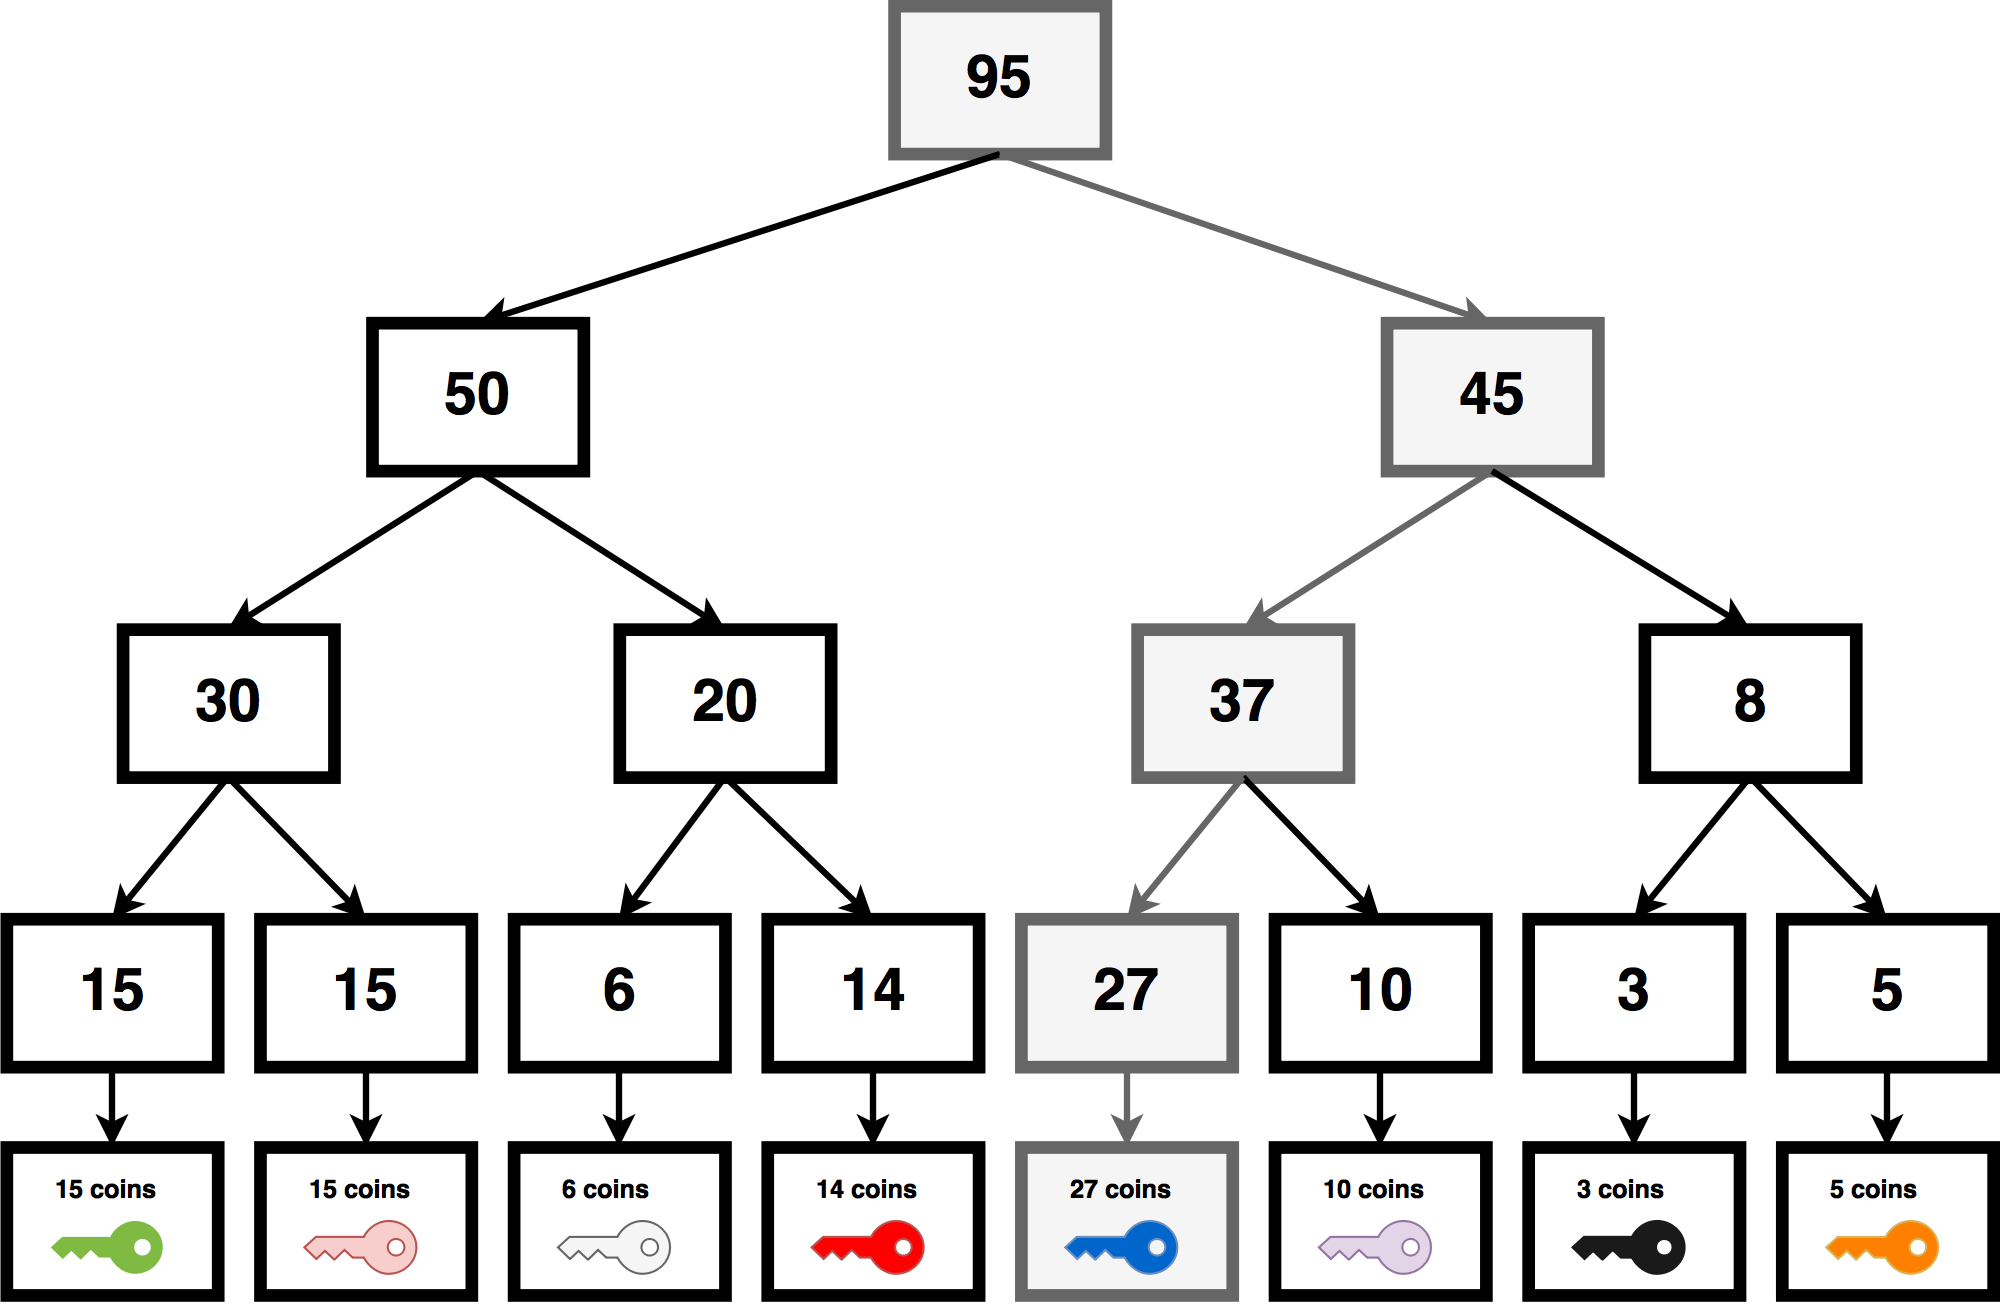
\includegraphics[width=\textwidth]{figures/stake-tree}
    \caption{An example of a stake tree with 8 stakeholders $\mathcal{A}_1, \mathcal{A}_2\ldots \mathcal{A}_8$. The nodes highlighted in grey are the nodes visited after a follow-the-satoshi where stakeholder $\mathcal{A}_5$ was chosen as the next block leader. The stake tree is created bottom-up fashion where each node in the tree is labelled with the sum of coins for its two child nodes.}
    \label{fig:stake-tree}
\end{figure*}

\subsection{Follow-the-satoshi in the Stake Tree}
\label{fts-tree}
We can do a follow-the-satoshi in the stake tree, as in \cref{alg:fts-tree} from \cref{fts-appendix}, by traversing the tree down to a leaf node, starting at the root as follows: Begin by initialising a CSPRNG $\Re(M) \rightarrow [1, M]$ with a seed $s$. Given a node with two child nodes, labelled with $x_1$ and $x_2$ indicating the amount of coins in the left and right subtree respectively, generate a new random number $r \gets \Re(x_1 + x_2)$. Choose the left subtree if $1 \le r \le x_1$, or choose the right subtree if $x_1 < r \le x_1 + x_2$. Follow-the-satoshi terminates when a leaf node has been reached, containing the account $\mathcal{A}_i$ of the winning stakeholder. Psuedocode is available in \cref{fts-appendix}.

\begin{lemma}[Follow-the-satoshi is fair]
Follow-the-satoshi in a stake tree with $N$ stakeholders and $\sum_{i=1}^{N}{x_i}$ coins selects the $k$-th stakeholder $1 \le k \le N$ with $x_k$ coins with probability $\frac{x_k}{\sum_{i=1}^{N}{x_i}}$.
\end{lemma}
\begin{proof}
We use structural induction. Only trees with depth $d$ and $N = 2^{d-1}$ leaf nodes are considered, since if $N$ is not a power of two, we can always fill the tree up with empty accounts, such that the condition holds.

\noindent
\textbf{Base case} The base case is a tree with a single node, containing an account $\mathcal{A}$ with $x_1$ coins. Since Follow-the-satoshi always selects an account, and there is only one account to choose from, it selects $\mathcal{A}$ with probability $1 = \frac{x_1}{x_1} = \frac{x_1}{\sum_{i=1}^{1}{x_i}}$.

\noindent 
\textbf{Induction hypothesis} Suppose follow-the-satoshi selects the $k$-th stakeholder with probability $\frac{x_k}{\sum_{i=1}^{N}{x_i}}$ $\forall \mathbb{T'} : |\mathbb{T'}| \le 2^{d} - 1$.

\noindent \textbf{Inductive step} Let $\mathbb{T'}_1$ and $\mathbb{T'}_2$ be two trees of of depth $d$ and construct a new tree $\mathbb{T} = \mathsf{Tree}(\mathbb{T'}_1, \mathbb{T'}_2)$ of depth $d + 1$. Denote by $\text{coins}(\mathbb{T})$ the total number of coins in the tree $\mathbb{T}$.

\begin{align*}
P(\text{account~}k) = P(\text{subtree~} \mathbb{T'}_x) \cdot P(\text{account~}k\text{~in~}\mathbb{T'}_x) \underset{\text{IH}}{=} \\ \frac{\text{coins}(\mathbb{T'}_x)}{\text{coins}(\mathbb{T})} \cdot \frac{x_k}{\text{coins}(\mathbb{T'}_x)} = \frac{x_k}{\text{coins}(\mathbb{T})}    
\end{align*}

\noindent Since the induction hypothesis holds for the larger stake tree $\mathbb{T}$, it holds for all stake trees.
\end{proof}

\subsection{Operations on the Stake Tree}
\label{stake-tree-operations}
Operations on the stake tree, allow stakeholders to transfer coins between each other, change the public keys, create new stakeholders, confiscate the coins of a malicious stakeholder and lock individual wallets as specified in \cref{app:stake-tree-transactions}. Locking wallets and confiscating coins of another stakeholder is done through voting. Each stakeholder has a voting power proportional to the amount of coins they own. A vote takes effect once a coalition of stakeholders controlling a majority of the coins has confirmed the vote. Each vote is timestamped to prevent an adversary from replaying an old vote.

\section{The Account Tree}
\label{account-tree}
The account tree is an authenticated, disk-based data structure which keeps track of all accounts at a certain block number. The account tree should fulfill the following requirements:

\begin{itemize}
\item It should be as compact as possible to store on disk, to minimise the storage requirements for a full node.
\item There should be mechanism for detecting expired accounts, to remove them from the tree and reclaim disk space.
\item Insertions and deletions in the account tree should be fast, something like $\mathcal{O}(\log n)$, in order to quickly process operations on the account tree, such as purging expired accounts, add new accounts and perform key updates.
\item The data structure should offer a small (no more than a few KB) proof of existence for an account in the tree.
\end{itemize}

A common way of storing ordered sets is by the use of trees which offers fast removal and insertion. Such data structure can easily be converted into an authenticated data structure using a dynamic Merkle tree as explained in \cref{sec:dyn-merkle}. To keep the Merkle proofs small, one should use trees with bounded depth and a small branching factor, ideally some sort of binary self-balancing tree. Thus, we suggest the account tree to be based on a dynamic Merkle tree, ordered by account name hash $H(\mathcal{N})$.

The accounts are put in interior nodes and the rotations of the tree dictates how the Merkle tree should be modified when account are added or removed. To be able to detect expired accounts and remove them from the tree, it is accompanied with a min-heap, ordered by date of expiry found in the CA proof as shown in \cref{fig:account-tree}. The account tree must be updated equally by all nodes, such that everyone arrives at the same Merkle root hash.

\begin{figure*}
    \centering
    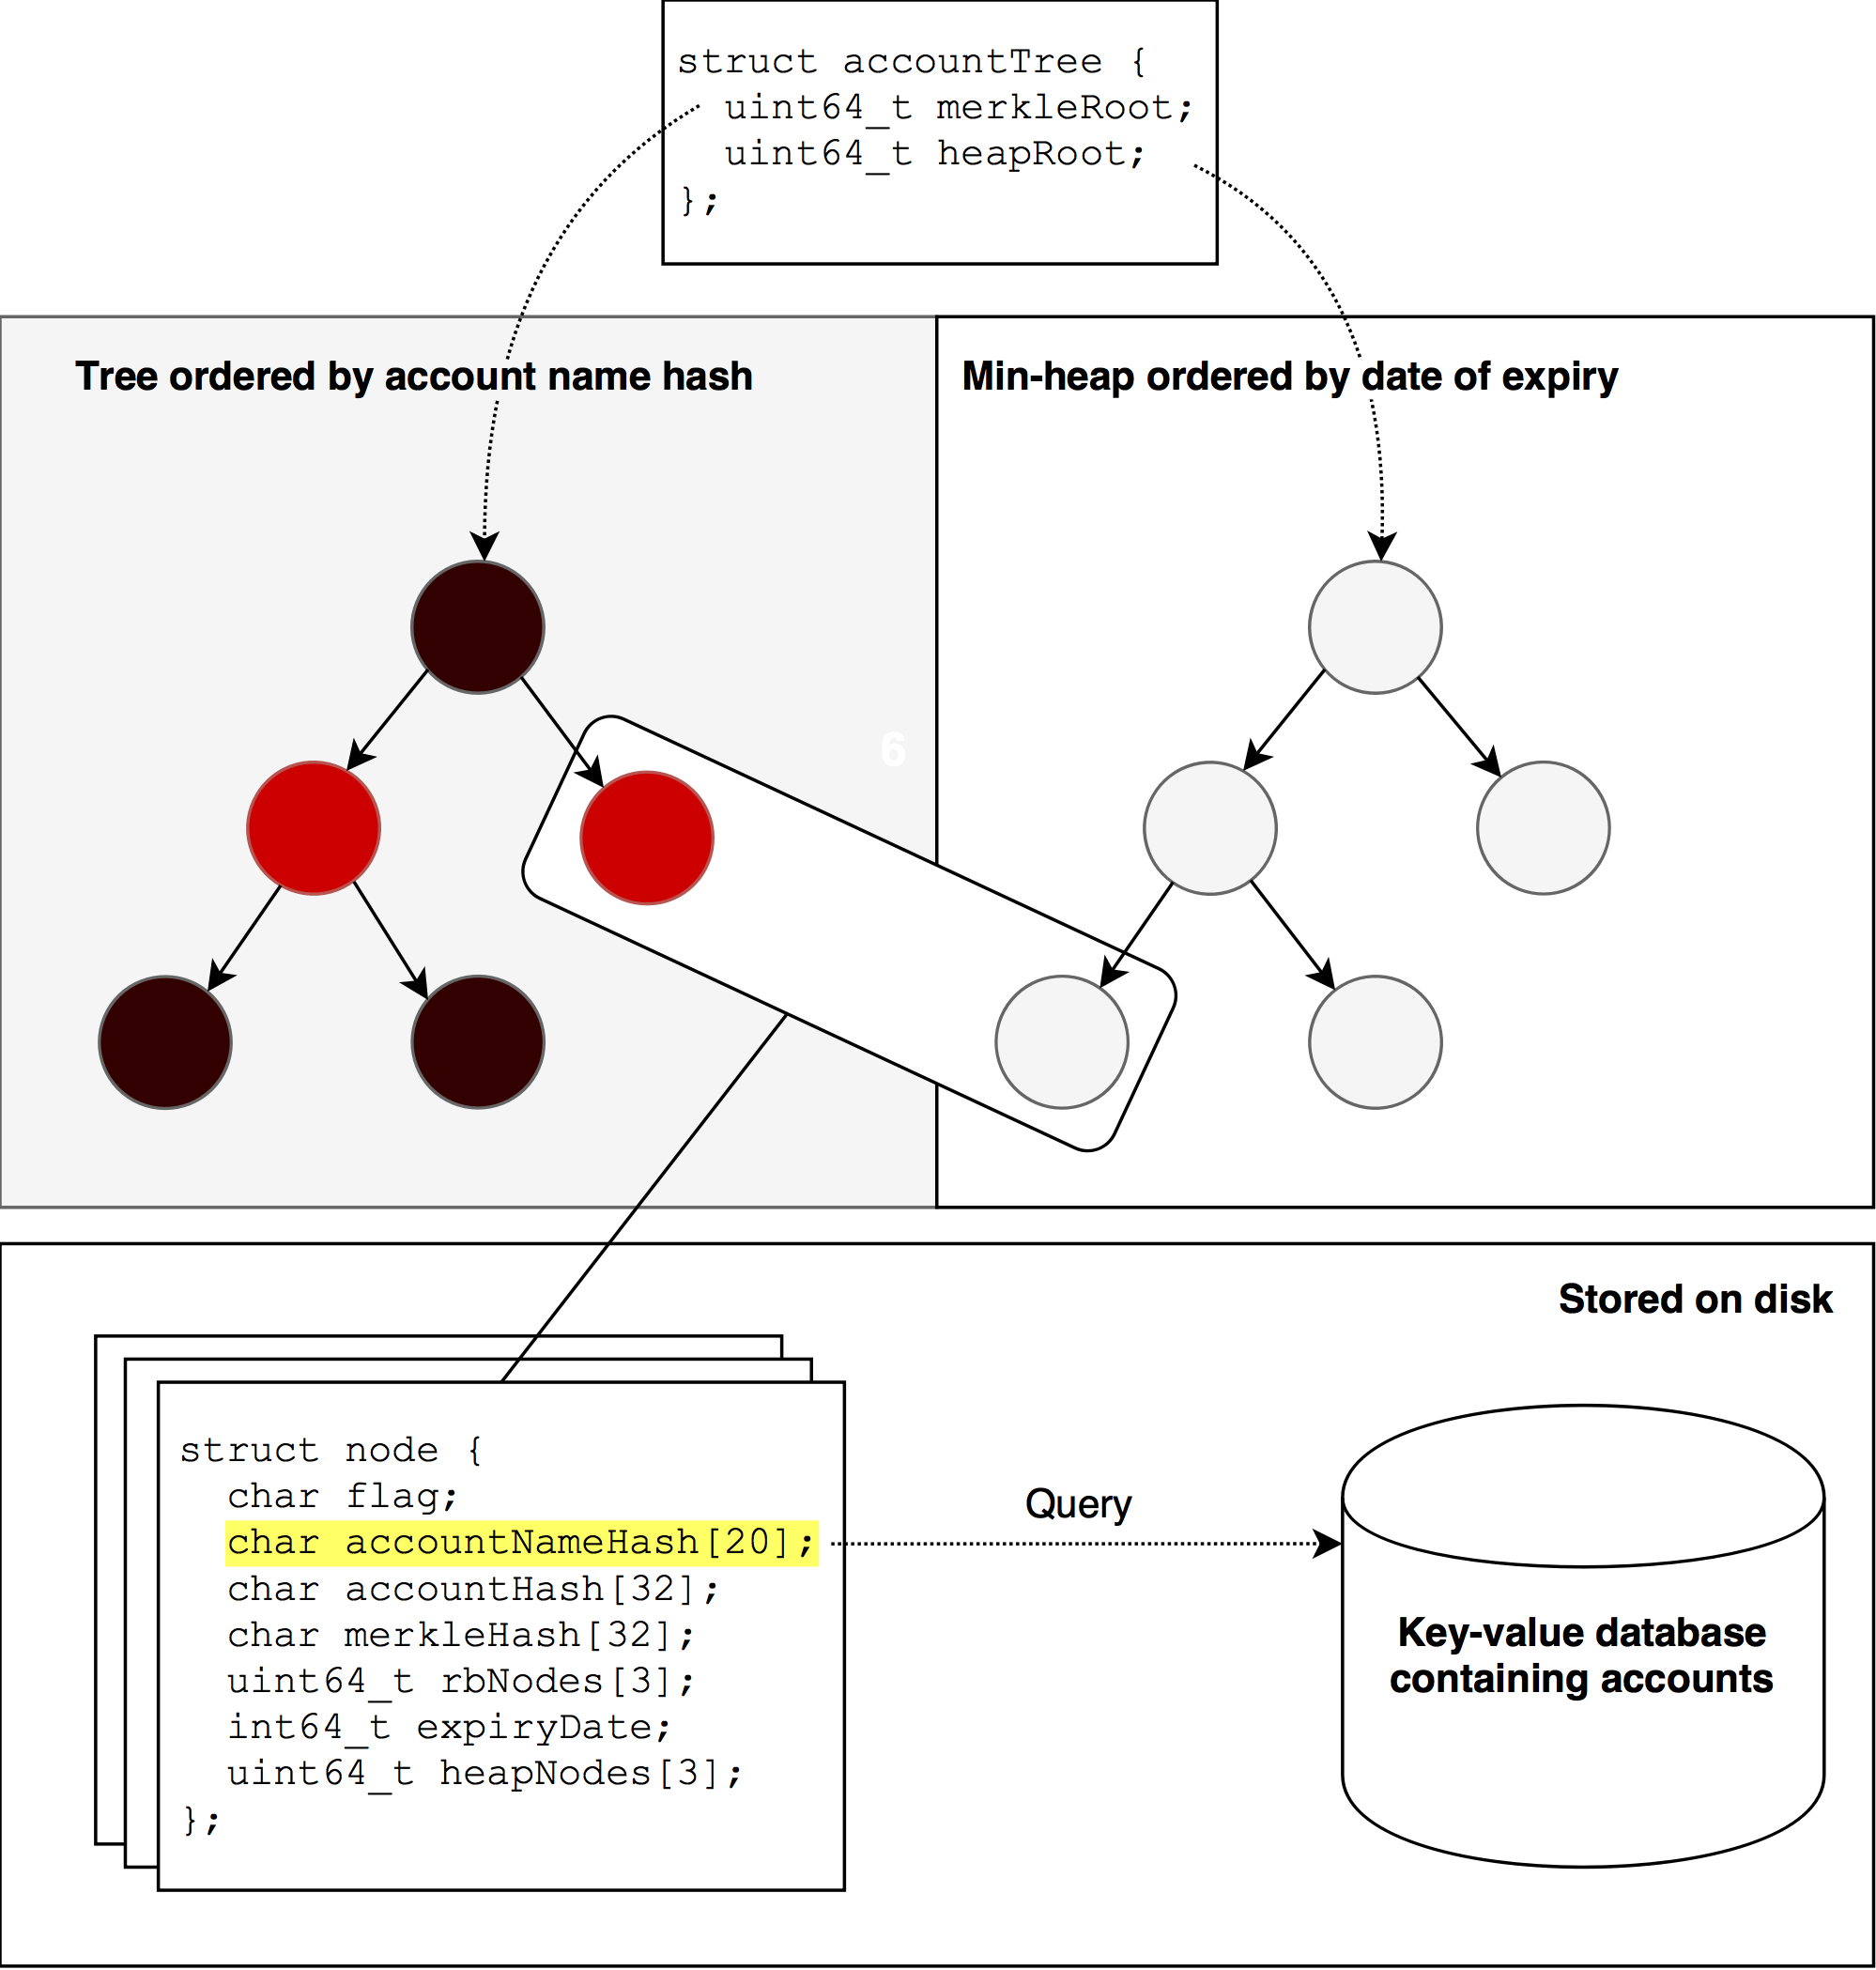
\includegraphics[width=\textwidth]{figures/account-tree}
    \caption{An example of an account tree with five accounts, modeled as a Merkle tree on top of a self-balancing binary tree ordered by account name hash $H(\mathcal{N})$, together with a min-heap ordered by account expiry date. The purpose of the min-heap is to quickly detect and prune expired accounts. Nodes for the two trees are stored in disk blocks, where each disk block represents a pair of nodes, one node from the self-balancing tree, and the corresponding node in the min-heap. The actual account contents (such as scripts) are stored in a key-value database.}
    \label{fig:account-tree}
\end{figure*}

Our account tree should implement the following methods:

\begin{itemize}
    \item $\mathsf{Lookup}(\mathcal{N}) \rightarrow (\mathcal{A}, \mathcal{P})$ performs a lookup for an account with account name $\mathcal{N}$, and returns the account $\mathcal{A}$ and Merkle proof $\mathcal{P}$ for a particular block or $\bot$ if the account does not exist.
    \item $\mathsf{Insert}(\mathcal{A})$ inserts a new account $\mathcal{A}$ into the account tree, iff the account does not already exist.
    \item $\mathsf{Delete}(\mathcal{N})$ deletes the account with account name $\mathcal{N}$.
    \item $\mathsf{Prune}(\mathcal{D}_{\text{now}})$ Delete accounts from the account tree whose expiration date $\mathcal{D} \ge \mathcal{D}_\text{now}$.
    \item $\mathsf{Update}(\mathcal{A})$ updates an account with the new information contained in $\mathcal{A}$.
\end{itemize}

\subsection{Operations on the Account Tree}
Operations on the account tree allow users to manage their digital identity in our distributed PKI, namely to add new identities and renew, revoke and change the keys of existing identities as specified in \cref{app:account-tree-transactions}. Each operation is a transaction which must contain a valid unlocking script fulfilling the conditions specified in the update or revocation script. In addition, adding a new identity or changing an existing identity requires a signature produced by a CA. As a consequence, an adversary trying to impersonate a user in our system, must not only be in control of a CA, but also have access to the private keys of the user.

\section{The Blockchain Truststore}
The blockchain truststore is a truststore on the blockchain, containing the names and public keys of all CAs eligible to create CA proofs. The signatures in the CA proofs, submitted when accounts are added or updated, are then checked by blockchain nodes against this truststore, to determine the validity of the CA proof. If a blockchain node is unable to verify a signature using the specified public key, or if the signature is produced by a CA not active in the blockchain truststore, the CA proof must be rejected and the transaction should be dropped.

The blockchain truststore is an append-only file whose hash is stored in the block header of each keyblock. The integrity of the truststore can be checked by comparing the hash of the truststore to the hash stored in the block header of the last keyblock. The truststore can be updated by adding new CAs, or revoke trust in existing CAs as specified in \cref{app:truststore-transactions}. Any such change must be confirmed by a coalition of stakeholders, controlling a majority of the coins in the stake tree.

When a CA is added, it is assigned an unused ID, and a timestamp of creation together with the public key of the CA is recorded in the truststore. If the CA is revoked, the time of revocation is recorded, but the entry is kept in the truststore to make it possible for blockchain nodes to validate old CA proofs.

Since entries are never removed from the truststore, the size of the file is going to grow over time. However, considering revocation of a CA is an unusual event, we do not anticipate this to be a problem.

\section{Keyblocks and Microblocks}
We distinguish between keyblocks and microblocks, specified in \cref{app:block-format}. Keyblocks contains transactions for the stake tree and blockchain truststore and microblocks contains transactions for the account tree. Like in Bitcoin-NG \cite{Eyal15}, a keyblock signals the change of a block leader and is followed by one or more microblocks. Since consensus is based on Proof of Stake instead of Proof of Work, both keyblocks and microblocks are signed with the private key of the stakeholder and each keyblock contains an output from \cref{alg:fts-tree} in \cref{fts-appendix} which can be used to validate the block without downloading the stake tree. The nonce and difficulty target fields are removed since they are not needed, and a reference to the previous keyblock is added in addition to a reference of the previous block. This makes it possible for thin clients to drop intermediary microblocks and only validate the keyblocks. Unlike Bitcoin, each keyblock also contains a hash of the blockchain truststore, and a Merkle root hash of the account tree. The coinbase transaction is removed since no block reward is given for creating new blocks.

\subsection{Dynamic Block Size}
\label{dyn-block}
Bitcoin features a hard-capped 1 MB block size limit, which would require a hard fork to change. Such a hard fork would be inconvenient to do since it would require all participants in the network to upgrade their software. A hard fork might also lead to a consensus failure if some stakeholders refuse to update. To avoid such a situation, while enabling the network to dynamically scale when the number of users increases, one could have a dynamic block size which can be changed by stakeholders through voting (\cref{tab:change-blocksize}). This allows us to regularly adjust the maximum throughput of the system.

\begin{table*}
\caption{A $\mathsf{ChangeBlocksize}$ transaction proposing a new block size for the next epoch.}
\label{tab:change-blocksize}
\begin{tabularx}{\textwidth}{lXl}
\cmidrule(r){1-3}
Field & Description & Size \\ 
\cmidrule(r){1-3}
\textbf{Origin} & A hash $H(\mathcal{N})$ identifying the voting stakeholder. & $32$ bytes \\
\textbf{New block size} & The proposed block size in bytes. & $4$ bytes \\
\textbf{Unlocking script} & A Bitcoin unlocking script authorising this transaction. & VarInt \\
\end{tabularx}
\end{table*}

\section{Epochs, Timeslots and Block Leaders}
To elect a new block leader, we use an approach inheriting many of its features from the Ouroboros Proof of Stake protocol. Time is divided into epochs, where each epoch consists of $2n$ consecutive keyblocks. An epoch is further split into timeslots. Before starting a new epoch, \cref{alg:fts-tree} is used as explained in \cref{fts-tree} to sample a list of $n$ lucky stakeholders, eligible to produce blocks during their designated timeslot. When a new timeslot starts, the next stakeholder (as chosen by \cref{alg:fts-tree}) broadcasts a new keyblock to the network. This stakeholder is then allowed to confirm transactions by producing microblocks until the timeslot ends and another stakeholder takes over. A timeslot can be seen as the equivalent to Bitcoin's block interval, but is always fixed to say 10 minutes. See \cref{app:blockchain-operation} for details.

\begin{definition}[Longest chain]
The longest chain in our distributed PKI is the chain with the most keyblocks.
\end{definition}

An epoch is divided into a commit phase and a reveal phase as shown in \cref{fig:pos}. The block leaders are the same in both the commit and reveal phase, and one could think of the reveal phase as a repetition of the commit phase with only one small difference as follows: In the commit phase, each keyblock should contain a commitment $H(\mathcal{R})$ to a $128$ bit random value $\mathcal{R}$ which is put into the block header. In the reveal phase the same block leader reveals the committed value by putting $\mathcal{R'}$ in the block header of the keyblock, such that $H(\mathcal{R'}) = H(\mathcal{R})$. The revealed values $\mathcal{R}_1, \mathcal{R}_2\ldots \mathcal{R}_{\frac{n}{2}}$ are then mixed together, to produce a seed for the CSPRNG used as input to \cref{alg:fts-tree}.

Our protocol uses a single block leader at a time, meaning the blockchain network would be unable to confirm transactions if a stakeholder is offline during their timeslot. This problem does not occur in Bitcoin where all miners are competing against each other to create the next block. To mitigate this problem, one could have a more complex protocol with multiple block leaders, but this is not investigated in this thesis. Instead, we instead rely on stakeholders to be online when their timeslot arrives, and a few instances of unavailability could be corrected by using a flexible block size.

\begin{figure*}
    \centering
    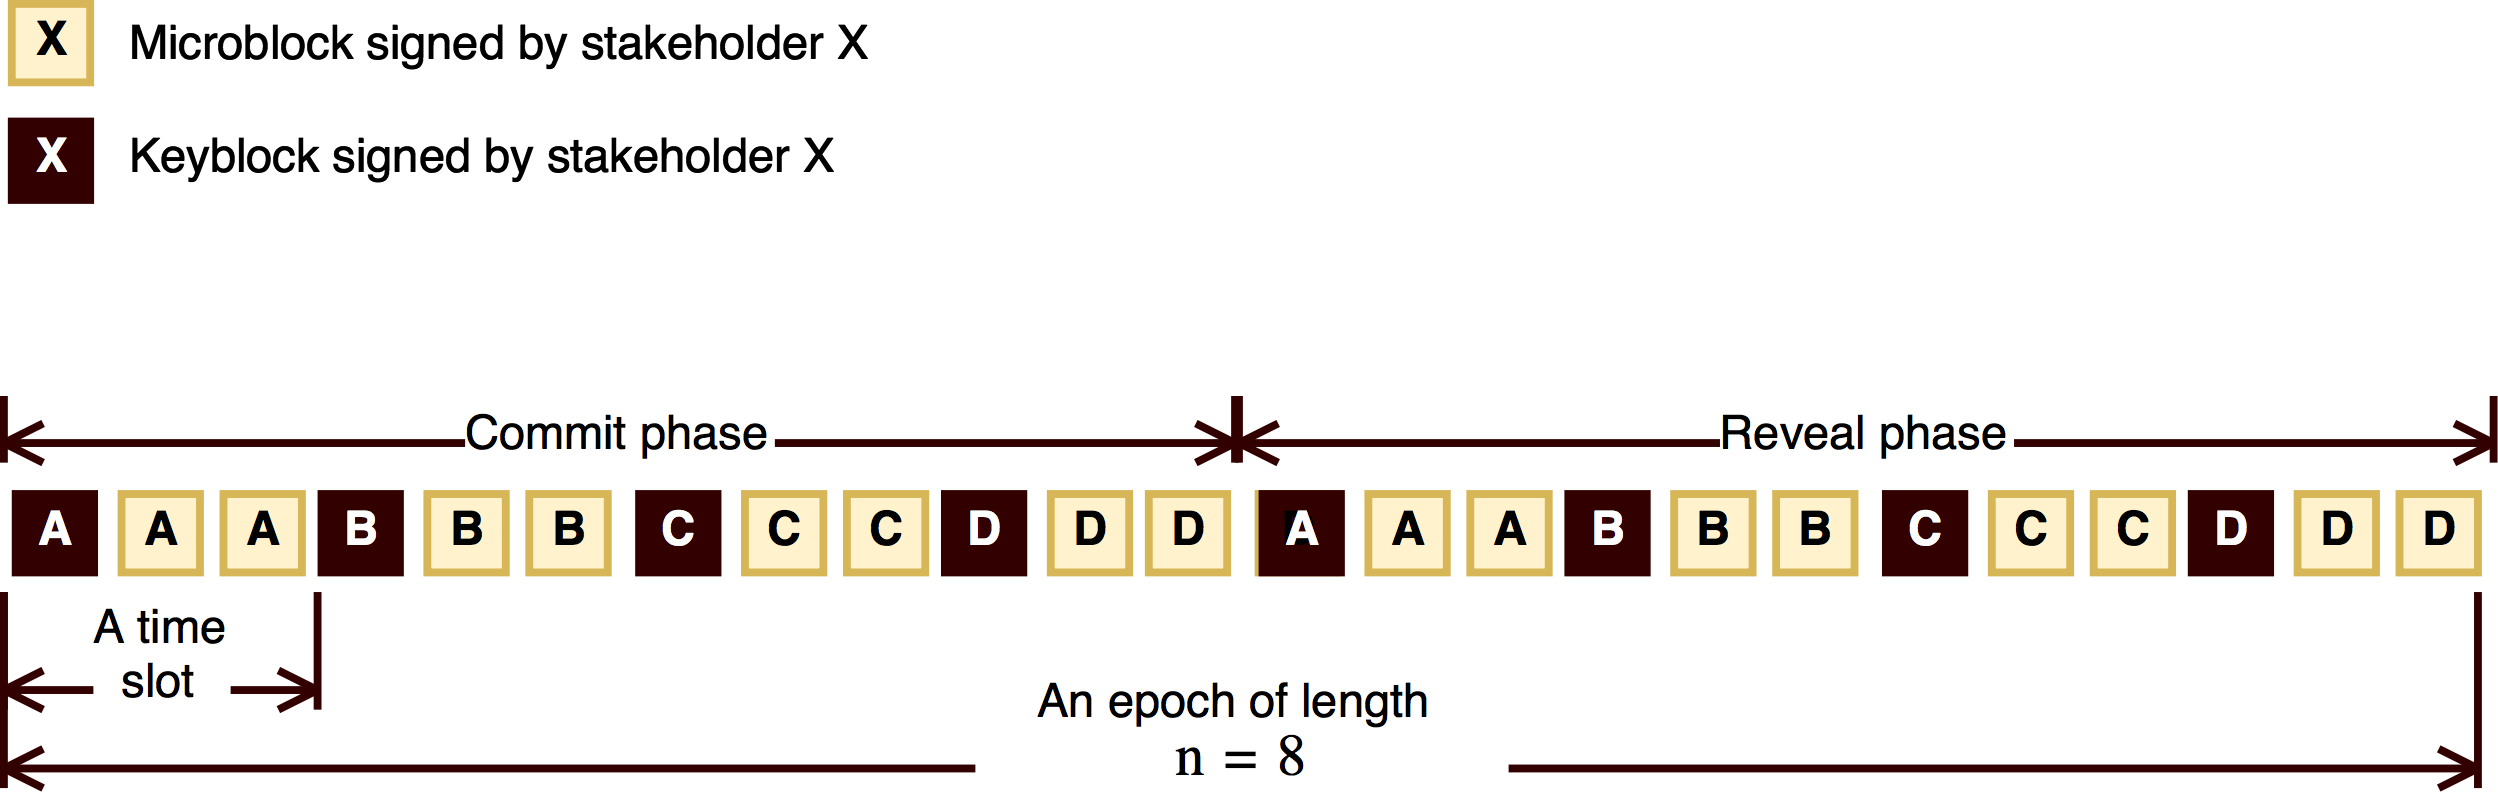
\includegraphics[width=\textwidth]{figures/proof-of-stake}
    \caption{Time is divided into epochs consisting of timeslots. Each timeslot is reserved for one block leader, chosen by a follow-the-satoshi performed on the stake tree, described in \cref{alg:fts-tree} (\cref{fts-appendix}). The epoch consists of a commit phase, where each block leader commits to a random value, and a reveal phase where this random value is revealed. The random values are then mixed together at the end of the epoch, and the result is used to reseed the CSPRNG used by \cref{alg:fts-tree} to sample block leaders for the next epoch.}
    \label{fig:pos}
\end{figure*}

\section{Co-signing Keyblocks}
To avoid waiting for several confirmations before the content of a block is accepted, which inevitably leads to delays in the system, each keyblock must be co-signed by a quorum of block leaders elected during an epoch. As a consequence, it also becomes more difficult to create a fork or sign an invalid keyblock. To achieve this, two additional fields are required in the block header: a bit array indicating which block leaders who have co-signed the block and a list of signatures. \cref{app:block-format} assumes the signatures can be aggregated and stored in a single field to reduce the size of the block header.

\chapter{Identity Management}
\label{chap:identity}
This chapter explains the issuance, revocation and verification process of accounts in the account tree and certificates issued by CAs, using the blockchain in the previous chapter. A client can verify a certificate in two ways, either by running its own blockchain node which maintains a complete keystore, or by running a thin client which retrieves the correct public key when required.

\section{Manage Accounts in the Account Tree}
Accounts are added, updated or removed by transactions posted to the blockchain network, as specified in \cref{app:account-tree-transactions}. Each such transaction must be signed by a blockchain CA active in the blockchain truststore. This acts as an additional security barrier which makes it more difficult for an adversary to impersonate a domain owner whose private keys have been exposed.

An account in the account tree is created after a request from a domain owner, who sends the DNS domain name $\mathcal{N}$ to be registered on the blockchain, together with the account's update script $\mathcal{U}_\text{scr}$, revocation script $\mathcal{R}_\text{scr}$ and signing key $\mathcal{K}_S$ to their favourite blockchain CA. The domain owner must trust this blockchain CA to carry out the registration properly on their behalf. When the blockchain CA has convinced itself that the domain owner is the lawful owner of the claimed domain name and that the information submitted is correct, it creates a CA proof containing a CA identifier $\text{CA}_\text{OID}$, a creation date $\mathcal{T_C}$, a date of expiry $\mathcal{T}_E$, and a CA signature $\text{Sig}_\text{CA}$ as specified in \cref{tab:ca-proof}. This CA proof is then bundled with the information submitted by the domain owner and a transaction is broadcast to the blockchain network. At this point, no part of the transaction can be changed since this would break the CA signature.

\begin{table*}[t]
\caption{The contents of a CA proof which is used to authorise changes to the account tree. The CA proof can be though of as a ``lightweight blockchain certificate'' and is only 84 bytes in size.}
\label{tab:ca-proof}
\begin{tabularx}{\textwidth}{lXl}
\cmidrule(r){1-3}
Field & Description & Size \\ 
\cmidrule(r){1-3}
\textbf{CA identifier} & An object identifier $\text{CA}_{\text{OID}}$ indicating the name of the CA who created the CA proof. & $2$ bytes \\
\textbf{Creation date} & A UNIX timestamp indicating the time when the CA proof was signed. & $8$ bytes \\
\textbf{Date of expiry} & A UNIX timestamp indicating the date of expiry for the CA proof. & $8$ bytes \\
\textbf{Signature algorithm} & An OID indicating the algorithm used to produce the signature. & $2$ bytes \\
\textbf{CA signature} & A CA signature attesting to the validity of the CA proof. & $64$ bytes\footnotemark 
\end{tabularx}
\end{table*}

\footnotetext{Assuming ECDSA with a 256-bit elliptic curve is used.}

\section{Issuing and Revoking Certificates}
Certificates can be issued by any CA as long as they are running software which supports our custom certificate extension explained below. Each certificate should be cross-signed by the domain holder's signing key $\mathcal{K}_S$ found on the blockchain. To request a new certificate, the domain owner signs the CN and the certificate's public key using $\mathcal{K}_S$ and includes this information in the CSR sent to the CA. This signature is then included in a custom certificate extension before the certificate is sealed by the CA. If the certificate extension is set as non-critical it may be ignored by older clients while more modern clients can use the domain owner's signature as an additional guarantee that the certificate was issued with the consent of the domain owner.

All previously issued certificates for a domain are automatically revoked once a domain owner changes its signing key $\mathcal{K}_S$ on the blockchain, since this invalidates the domain owner's signatures found in the old certificates. Thus, protocols such as OCSP may be considered redundant since revocation information is already included in the certificate. We refer the reader to \cref{chap:discussion} for further discussion on this topic.

\section{Certificate Verification}
A client receiving a certificate chain from a server, must not only check the signature produced by the CA, but also the signature produced by the domain owner. To do this, the client need to retrieve the domain owner's public key along with an additional Merkle proof which proves that the public key belongs to the top domain in the certificate. This is done by checking the Merkle proof against the ``Account tree hash'' field found in the most recent keyblock on the blockchain as described in \cref{app:verify-cert}. 

The Merkle proof changes whenever a new keyblock is added to the blockchain, which means this information cannot be included in the certificate itself. Instead, the Merkle proof needs to be downloaded separately. This can be done in two ways: Either the client runs its own validator node which verifies every transaction and stores a complete copy of the account tree. This would be very impractical for most home users, although a company may run its own local validator node which can be accessed on the company's intranet. 

Instead, a client may run its own thin client which only downloads and verifies the block headers of the keyblocks. When a thin client receives a certificate, it connects to the blockchain network and requests a Merkle proof from a stakeholder or validator. Since the Merkle proof is hard to fabricate, it can be supplied over an untrusted channel. To eliminate the need for a thin client to create a separate connection, the Merkle proof and the public key could be included in a custom OCSP response and be stapled with the certificate using OCSP stapling.

\chapter{Evaluation}
\label{chap:evaluation}
This chapter contains a summary of our findings and elaborates on the security and scalability of our PKI.

\begin{itemize}
    \item[\checkmark] \textbf{Identity retention} Each identity can only be updated or revoked by presenting a solution to the accounts locking script defined by the owner, and each certificate is cross-signed with a key residing in this account. This makes it very difficult to impersonate someone, since it would require an adversary to gain access to both a CA and the private keys of the domain holder.
    \item[\checkmark] \textbf{Expiration of old identities} The date of expiry for an account is set via a timestamp in the CA proof. Account which have expired according to this timestamp are removed from the account tree and can be forgotten by blockchain nodes.
    \item[\checkmark] \textbf{Key recovery} Any number of backup keys can be specified using a Bitcoin multisignature script.
    \item[\checkmark] \textbf{Transparency} All transactions on the blockchain are public and anyone can connect to the blockchain network and start to audit transactions.
    \item[\checkmark] \textbf{Backward compatible} Cross-signed certificates are breaking older clients if the server signature is put in a non-critical certificate extension.
    \item[\checkmark] \textbf{Thin client support} Clients who want to verify a certificate only need to synchronise the block headers to do so. They can then request the additional information required to verify the signature of a certificate by querying the blockchain network.
\end{itemize}

\section{Security Analysis}
Security for blockchain nodes looks different depending on how they operate. We distinguish between \emph{stakeholders} and \emph{validators} which enforce all rules of the protocol and \emph{thin clients} which only validates the block headers of the longest blockchain. An end-user is typically running a thin client, and must to some extent rely on the honesty of the stakeholders.

\subsection{Threat Model}
\label{sec:threat-model}
At any time instant, we assume that there are two coalitions of stakeholders, a malicious coalition controlling a $p$ fraction of the coins and an honest coalition controlling a $1 - p$ fraction of the coins. The stakeholders within a coalition are assumed to cooperate with each other, but not necessarily with the stakeholders from the other coalition if they can benefit from not doing so. We furthermore assume that a stakeholder is operational during the whole epoch in which they have been assigned a timeslot. Thus, the possibility of denial of service against individual stakeholders is largely neglected.

\subsection{51\%-attack}
Clearly, security cannot be achieved when $p > \frac{1}{2}$ since a malicious majority can confiscate the coins of the honest stakeholders and take complete control over the system. Thus, a 51\%-attack would be fatal to our blockchain PKI. To mitigate this type of attack, it is important to make a good initial selection of stakeholders, where the coins in the stake tree are spread out among several different participants who are unlikely to cooperate maliciously.

\subsection{Censor Transactions}
The malicious coalition of stakeholders could try to censor certain transactions, such that certain domain owners are unable to renew their account or update their keys. Since stakeholders take turns in processing transactions, this should not constitute a big problem. If transactions are approved in a first-come, first-served fashion, any lingering transactions are the first to be approved by an honest stakeholder, unless there is congestion in the network.

\subsection{Signing a Counterfeit Keyblock}
Tricking an end-user running a thin client into accepting a counterfeit public key controlled by an adversary can be done by creating a blockchain with more keyblocks than the blockchain created by the honest coalition, where the last keyblock has signed a fraudulent Merkle root containing the adversary's public key. The (invalid) substitution of the domain owner's public key would be detected by a stakeholder or validator, but not by a thin client since they do not check every transaction on the network.

Assume each keyblock must be signed by a two-third quorum (a common threshold in Byzantine fault tolerant systems) of stakeholders elected during an epoch for the blockchain network to accept it. If \cref{alg:fts-tree} elects $n$ stakeholders during an epoch, then the malicious coalition is said to be winning at any time instant if and only if the number of malicious stakeholders elected $> \frac{2n}{3}$.

This probability can be modeled using a binomial distribution. If the malicious stakeholders control $p$ fraction of the coins as explained in \cref{sec:threat-model}, then we may view one execution of \cref{alg:fts-tree} as a Bernoulli trial with adversary success probability $p$. Let $\mathbb{X}' \in [0, 1]$ be the stochastic variable denoting the outcome of aforementioned Bernoulli test, where $1$ means success (malicious stakeholder chosen) and $0$ denotes failure (honest stakeholder chosen). The malicious coalition can successfully sign a counterfeit keyblock if and only if $\mathbb{X} = \sum_{i = 0}^{n}{\mathbb{X}'_i} > \frac{2n}{3}$.

This probability is given by the Binomial CDF:
\begin{equation}
\label{equ:binom-cdf}
\text{Pr}\Bigg( \mathbb{X} > \frac{2n}{3} \Bigg) = 1 - \sum_{i = 0}^{\frac{n}{2}}{{\binom{n}{i}} \cdot p^i \cdot (1 - p)^{n - i}} % < \underbrace{\mathsf{exp}\Bigg(-n\Big(p - \frac{2}{3}\Big)^2\Bigg)}_{\text{Chernoff bound}}
\end{equation}

For 128-bit of security and $p = 0.3$, one should choose $n$ such that $\text{Pr}\Big( \mathbb{X} > \frac{2n}{3} \Big) < 2^{-128}$. The smallest $n$ fulfilling this condition is $n = 120$, which means that an epoch must consist of at least $2n = 240$ timeslots.

\subsection{Stake Grinding}
As explained in the previous section, for $p = 0.3$ and $n = 120$, the probability for the malicious coalition to successfully sign a counterfeit block is negligible. However, this assumes \cref{alg:fts-tree} is fair, which might not be the case if the seed to the CSPRNG is controlled by an adversary. The malicious coalition can mount a stake grinding attack where they ignore the keyblocks produced by the honest coalition which gives them complete control over the input to the mixing function. They can then test many different $x_{i \in \mathbb{Z}_{128}}$ such that the seed $\mathsf{Mix}(x_{0 \le i < 2^{128}})$ gives them an advantage during the next epoch. This type of attack can be alleviated in different ways:
\begin{itemize}
    \item Make the mixing function time or memory consuming to compute. However, this may also lead to slow verification of blocks, which is undesirable.
    \item Make the mixing function hard to precompute, for example by using a hash of the block headers as salt.
    \item Increase the number of timeslots during an epoch. However, this would also lead to slower updates to the stake tree.
    \item Automatically lock the wallet of stakeholders who create an invalid keyblock.
\end{itemize}

\subsection{Compromised Stakeholder}
If a block signing key is compromised, it can be changed by posting a $\mathsf{SetSigningKey}$ transaction to the blockchain, signed by the keys referred in the stakeholder's locking script. If the keys referred in the stakeholder's locking script are compromised, an honest coalition of stakeholders can cooperate to revoke trust in the compromised stakeholder by posting a $\mathsf{ConfiscateStakes}$ transaction on the blockchain.

\subsection{Compromised Domain Owner}
An adversary who gets access to the private signing key of a domain holder can trick (any) CA to sign a fraudulent certificate on behalf of the adversary. However, this certificate can only be used until the domain owner detects the leak (for example by monitoring the CT logs) and changes its signing key by posting an $\mathsf{UpdateTransaction}$ on the blockchain. If the private keys referred in the domain owner's locking script are leaked and they trick a blockchain CA into approving a new locking script for the domain owner containing private keys controlled by an adversary, access to the domain is irrevocably lost. The domain owner must then wait until the account expires, and then re-register the account.

\section{Performance Analysis}
\label{performance-analysis}
This performance analysis provide some back-of-the-envelope calculations which is used to estimate resource requirements for blockchain nodes. The goal is to determine a suitable block size and make a verdict whether our scheme is practically applicable, if deployed on the same scale as DNS. Our analysis focuses on the the performance metrics discussed in \cref{scalability-concerns}.

The reason we choose to look at DNS, is because there is one-to-one mapping between domain names and accounts in the account tree. This means that the size of the account tree, and the number of transactions in the blockchain network is directly proportional to the number of domains. It should be noted that far from all domains utilise HTTPS today, but considering HTTPS is being more and more of a requirement, this is likely to change. 

\subsection{Block Size}
Based on statistics collected by VeriSign, there were a total of 327 million registered domain names across all top domains, at the end of the third quarter 2016, with an average yearly increase of about 23 million domain names per year between the years 2011 to 2016 \cite{VeriSign16}. 

\pgfplotstableread[col sep=comma]{
    date, variable
    2011 Q1, 210
    2011 Q2, 215
    2011 Q3, 220
    2011 Q4, 225
    2012 Q1, 233
    2012 Q2, 240
    2012 Q3, 246
    2012 Q4, 252
    2013 Q1, 256
    2013 Q2, 261
    2013 Q3, 265
    2013 Q4, 271
    2014 Q1, 274
    2014 Q2, 280
    2014 Q3, 284
    2014 Q4, 288
    2015 Q1, 294
    2015 Q2, 296
    2015 Q3, 299
    2015 Q4, 314
    2016 Q1, 326
    2016 Q2, 334
    2016 Q3, 327
    dummy, 350
}\datatable
\begin{figure*}
\begin{tikzpicture}
\begin{axis}[
    enlargelimits=0.030,
	legend style={at={(0.5,-0.1)},
	anchor=north,legend columns=-1},
	ybar interval=-0.5,
    height=10cm,
    width=\textwidth,
    enlarge y limits=false,
    ymin=200,
    ymax=350,
    ylabel=Number of domains $\times 10^6$,
    xtick=data,
    xticklabels from table={\datatable}{date},
    x tick label style={rotate=55, anchor=east},
    ymajorgrids=true,
    yminorgrids=true,
    minor tick num=2,
    xmajorgrids=false,
    xminorgrids=false,
]
\addplot [fill=blue] table [x expr=\coordindex, y=variable] {\datatable};
\end{axis}
\end{tikzpicture}
\caption{The number of domains registered in the domain name system, measured quarterly from the first quarter 2011 until the third quarter 2016.}
\label{fig:dns-scale}
\end{figure*}

Domains are typically registered and renewed on a yearly basis, and under the assumption that each registered domain name is either renewed or revoked once per year, a total of 327 million transactions must be processed every year, or 6000 transactions during a 10 minute timeslot. Assuming an average transaction size of 864 bytes (an update transaction with 128-byte account name, 320-byte unlocking script, 84-byte CA proof, 32-byte signing key, 160-byte update script and 160-byte revocation script\footnote{A multisignature script with five public keys is about 160 bytes large. This script should be versatile enough for most users.}) we need a block size of $5.2$ MB, split among several microblocks, about five times the current Bitcoin block size. A sudden increase of the number of transactions in the short run can be handled by queuing transactions in the mempool. However, once the mempool is full, one would have to drop transactions in the network. This is why renewals of domains have to be somewhat evenly spread out. To have everyone renewing their blockchain identity at the beginning of a new year would not work.

\subsection{Storage Requirements for Validators and Stakeholders}
Assuming each node in the account tree contains a 564-byte account (consisting of 128-byte account name, 32-byte signing key, 84-byte CA proof, 160-byte revocation script and 160-byte update script): a database with all 327 million accounts would have a size of $\approx 185$ GB. Blockchain nodes would also have to store the account tree, consisting of the min-heap and self-balancing tree discussed in \cref{account-tree}. If each disk block for this account tree is 109 byte large, the whole account tree structure would occupy another $36$ GB. 

Additionally each node may have to store a synchronisation point consisting of all transactions for the last $w$ blocks, together with an old version of the account database and the account tree, as it looked $w$ blocks ago. Not all nodes need to store this information, since it is only needed to bootstrap new nodes. Say for example, that each epoch consists of $160$ keyblocks, and by convention each blockchain node stores the transactions of the last 30 epochs. With a block interval of 10 minutes as in Bitcoin, this is all transactions during a one-month period. This would occupy an additional $22$ GB for the transactions and another $216$ GB for the account tree and the database. 

Storage requirements would increase over time when more and more accounts are added. Assuming linear growth with 23 million accounts every year, the size of the database would increase with about 13 GB/year, the one-month transaction set would increase with 1.65 GB/year and the account tree would increase with 2.5 GB/year. A summary is available in \cref{tab:storage}.

\begin{table*}
\ifbook
\scriptsize
\fi
\label{tab:storage}
\caption{Storage and bandwidth requirements for different blockchain nodes.}
\begin{tabularx}{\textwidth}{XXXX}
\textbf{Data} & \textbf{Stored/downloaded by} & \textbf{Size} & \textbf{Growth} \\
\cmidrule(r){1-4}
Account tree & Validators and stakeholders & 36 GB & 2.5 GB/year \\
Account contents (such as scripts) & Validators and stakeholders & 185 GB & 13 GB/year  \\
Transaction history & Stakeholders and some validators & 22 GB/month & 1.65 GB/year \\
Synchronisation point & Stakeholders and some validators & 243 GB & 17.15 GB/year \\
Block headers & Everyone & 13.6 MB/year & \\
Stake tree & Everyone & Negligible & Negligible \\
Blockchain truststore & Validators and stakeholders & Negligible & Negligible \\
Proof data & Thin clients & 3.7 KB/certificate & \\
\end{tabularx}
\end{table*}

\subsection{Bandwidth Requirements for Thin Clients}
Thin clients need to download a copy of the stake tree and the block headers of the keyblocks. They can then request a Merkle proof from a validator or stakeholder when required, to convince themselves that a certain account is present in the account tree.

The size of a keyblock is 251 bytes during the commit phase and 267 bytes during the reveal phase as specified in \cref{app:block-format}. With a block interval of 10 minutes, this yields about 13.6 MB of block headers every year, which has to be downloaded by new clients. The size of the stake tree grows over time when new stakeholders are added and removed, but unless this happens very often, the size of the stake tree should remain negligible.

In addition to the bandwidth required to download the block headers and the stake tree, which is only done once, a thin client also need to download the server's public key and some proof data for each certificate it want to validate. More specifically, they need to download the blockchain account for a domain holder together with a Merkle proof which proves that the account is present in the account tree. If the account tree is implemented using a red-black tree, the Merkle proof will be of bounded size as follows: 

\begin{lemma}[Maximum depth of a red-black tree]
The depth of a red-black tree with $n$ nodes is bounded by $\mathcal{O}(\log n + 1)$.
\end{lemma}

Hence, the depth of an account tree containing all 327 million domains is at most 57. For each level in the tree, two hashes are needed to recreate the Merkle hash of the parent node (the Merkle hash of the sibling node and the hash of the account stored in the parent node). If each hash is 32 bytes, this means that the maximum size of any Merkle proof will be $\approx 3.7$ KB. Additionally, one would have to send the domain owner's public key and a hash of the account body, which can be used to compute the Merkle hash of the account (see \cref{account-hash}).

\subsection{Bootstrap Time for New Nodes}
A new blockchain node which is booting up needs to synchronise with the network before it can start to validate new transactions. This involves downloading and verifying the block headers of the longest available blockchain $B_1, B_2\ldots B_N$, downloading the accounts and the account tree for block $B_i$, $0 < i < N$ and all transactions for the most recent $N-i$ blocks $B_i, B_{i+1}\ldots B_N$. To download the account tree ($\approx 36$ GB), the account database ($\approx 185$ GB) and one month of transaction history ($\approx 22$ GB) would take about 11 hours with a 50 Mb/s internet connection. Since we always keep a window of only the last $N - i$ transactions, the time to bootstrap new nodes will not increase significantly over time.

\chapter{Discussion}
\label{chap:discussion}
The proposed design has mainly been motivated by scalability, which was deemed to be the largest obstacle for our blockchain-based solution to work. Although it appears as storage requirements are not going to be a large problem if pruning is used, the number of transactions which can processed is still a bottleneck. This could potentially be rectified by sharding the blockchain, meaning a transaction is only validated and stored by a subset of stakeholders. Sharding is a topic of ongoing research, and will probably have to be investigated in more detail before deploying our blockchain scheme at scale. Apart from throughput, we also faced issues with large block headers, mainly due to the use of Merkle proofs in our Proof of Stake scheme. Our block headers are significantly heavier than Bitcoin's, and occupies about 13.6 MB yearly, compared to Bitcoin's 4.2 MB. For full security, a client must synchronise these headers along with a copy of the stake tree before any certificates can be validated, which may prove cumbersome in practice.

It should be noted that the Bitcoin blockchain is almost trustless, while our system requires some trust in the stakeholders who maintain the blockchain. In particular, a majority of stakeholders can collude in order to subvert the integrity of the blockchain. We would argue that such an attack is unlikely to happen on purpose, since it most likely will be detected and the stakeholders involved may face legislative action as a result. Our system also requires some trust in the CAs responsible for signing CA proofs. A malicious blockchain CA could try to swap the keys of the domain owner before registering the identity. This would not pose a threat to already registered identities, but could still prove to be problematic since existing identities cannot be revoked. 

The owner of an identity is the owner to the keys referred in the account's locking script. If these keys are stolen or lost, there may be no way of recovering the account and one would have to wait until the account has expired and can be registered again. Ironically, this is also the strength of the blockchain since it is impossible to take control over someone's account without having access to their keys. However, one always have the opportunity to specify a separate revocation script, which can be used by for example a CA to re-register the account. Techniques such as Verifiable Secret Sharing where a key is split among several people, or the use of multisignature scripts containing backup keys can be used to ensure an account can be recovered even if some keys are lost. In this way, it is up to the domain owner to adjust the level of security to fit their needs.

A benefit of a distributed PKI is that it may have the potential to improve certificate revocation. In a distributed PKI, each domain owner would be able to attest to the validity of their own certificates. This eliminates the need for a centrally administered OCSP servers run by CAs, which can be a targets for denial of service attacks. However, it is doubtful whether our blockchain solution could provide reliable revocation services due to limited transaction throughput. Further work on the use of distributed PKIs for certificate revocation is a good topic for future research.

\section{Conclusion}
Although the use of a blockchain as an authoritative source of information for the web sounds tempting, mainly due to its strong security guarantees, it is not without drawbacks. Most notably, a client must synchronise the block headers of the longest chain before it can start to verify the server signatures found in certificates, and the limited number of transactions which can be processed may limit its usability. Although a block size of 5.2 MB is perfectly feasible, it assumes renewal of identities are evenly spread out during the year, which is somewhat unrealistic. A blockchain design would also discourage domain holders from using the blockchain as a tool for revocation, since this would lead to an increase in the number of transactions which has to be processed. In the unlikely event of a new Heartbleed bug, where millions of servers may need to rotate their keys at the same time, the system would simply grind to a halt. Identities which are lost, would also be unavailable until they expire which may discourage some people from putting their identity on the blockchain. 

These drawbacks indicate that a distributed PKI backed by a blockchain is not a silver bullet in its current form, but rather a complement to existing security solutions. At this stage, it is hard to predict whether a blockchain-based solution for the web will succeed. Success is largely going to depend on the participation of CAs, browser vendors and other stakeholders, and whether they can agree on a standard which can be widely adopted and implemented.

\ifbook
\begin{flushleft}
\bibliography{references}
\end{flushleft}
\else
\ifbook
\clearpage
\fi
\section*{About PrimeKey}
This thesis was written at \textbf{PrimeKey Solutions AB}. PrimeKey provides businesses and organisations around the world with the ability to implement security solutions such as e-Passports, authentication, digital signatures, unified digital identities and validation using EJBCA Enterprise, SignServer Enterprise and PrimeKey PKI Appliance. PrimeKey has its head office in Stockholm, Sweden.
\ifbook
\clearpage
\fi
\section*{Acknowledgements}
I want to thank PrimeKey for giving me the opportunity to write this thesis, specifically Johan Eklund and my PKI advisor Mike Kushner who have taken great interest in my work and provided me with useful feedback. I also want to thank everyone at my university who have helped me throughout the writing of this thesis, most notably my university advisor Dr. Per Austrin and my examiner Prof. Johan Håstad. I also want to mention the following students who have helped me peer review an earlier draft: Arash Safari, Edvin Lundberg, Hannes Leskelä, Lovisa Runhem and Martin Steier - thank you for your ideas and comments! Finally, I want to thank Dimaz Ankaa Wijaya for all interesting conversations about blockchains. 
\\\\
\begin{mdframed}[backgroundcolor=white,leftline=false,bottomline=false,rightline=false,innerleftmargin=0pt,innerrightmargin=0pt,innertopmargin=10pt,innerbottommargin=0pt]The most recent version of this thesis can be found at \texttt{\href{https://helix.stormhub.org/papers}{https://helix.stormhub.org/papers}.}
\end{mdframed}
\def\bibfont{\scriptsize}
\begin{flushleft}
\bibliography{references}
\end{flushleft}
\fi

\begin{appendices}
\ifbook \else \onecolumn \fi
\crefalias{chapter}{appsec}
\chapter{Follow-the-satoshi}
\label{fts-appendix}

This appendix contains psuedocode for \cref{alg:fts-tree}.

\begin{algorithm}
\caption{Procedure for follow-the-satoshi in a stake tree, taking a CSPRNG $\Re$ and a stake tree $\mathbb{T}$ as input, and outputs a wallet $\mathcal{W}$ chosen at random with probability proportional to the number of coins in the wallet. The stake tree is modeled as a one-indexed array where $\mathbb{T}[1]$ is the root of the tree. Each node $\mathbb{T}[i]$, $1 \le i \le |\mathbb{T}|$ is a tuple $(x_1, x_2, \mathcal{W})$ where $x_1$ is the total amount of coins in the left subtree, $x_2$ is the total amount of coins in the right subtree, and $\mathcal{W}$ is the wallet of a stakeholder or \texttt{nil} if the node is not a leaf node.}
\label{alg:fts-tree}
\begin{algorithmic}
\Procedure{$\text{fts-tree}(\Re, \mathbb{T}) \rightarrow \mathcal{W}$}{}
\State \textbf{assume~} $|\mathbb{T}| \ge 3$
\State $i \gets 1$ \Comment{index of root node}
\Loop
  \If{$\mathbb{T}[i]$ is a leaf}
    \State \Return $\mathbb{T}[i].{\text{wallet}}$
  \EndIf
  \State $x_1 \gets \mathbb{T}[i].{x_1}$
  \State $x_2 \gets \mathbb{T}[i].{x_2}$
  \State $r \gets \Re(x_1 + x_2)$
  \If{$1 \le r \le x_1$} \Comment{left subtree}
    \State $i \gets i \cdot 2$
  \Else \Comment{right subtree}
    \State $i \gets i \cdot 2 + 1$
  \EndIf
\EndLoop
\EndProcedure
\end{algorithmic}
\end{algorithm}

\chapter{Operations on the Stake Tree}
\label{app:stake-tree-transactions}
This appendix specifies the format of transactions related to the stake tree.

\begin{table*}[ht]
\caption{A $\mathsf{StakesTransfer}$ begins a transfer of coins by putting an encumbrance on an amount of coins with a locking script. The amount is transferred when someone presents a solution to the locking script provided in a matching $\mathsf{ReceiveStakes}$ transaction.}
\label{tab:transfer}
\begin{tabularx}{\textwidth}{lXl}
\cmidrule(r){1-3}
Field & Description & Size \\ 
\cmidrule(r){1-3}
\textbf{Payer} & A hash $H(\mathcal{N})$ identifying the stakeholder sending the coins. & $32$ bytes \\
\textbf{Payment script} & A Bitcoin locking script which defines the conditions which has to be fulfilled in order to complete the transfer using a consecutive $\mathsf{ReceiveStakes}$ transaction. & VarInt \\
\textbf{Amount} & The amount of stake to transfer. & $4$ bytes \\
\textbf{Timestamp} & A UNIX timestamp indicating the epoch for which this vote is valid. & $8$ bytes \\
\textbf{Unlocking script} & A Bitcoin unlocking script authorising this transaction. & VarInt
\end{tabularx}
\end{table*}
%%%%%%%%%%%%%%%%%%%%%%%%%%%%%%%%%%%%%%%%%%%%%%%%%%%%%%%%%%%%%%%%%%%%%%%%%%%%%%%%%%%%
\begin{table*}[ht]
\caption{A $\mathsf{ReceiveStakes}$ transaction receives coins from another stakeholder by presenting a solution to the corresponding payment script. This transaction requires a reference to a previously submitted $\mathsf{StakesTransfer}$ transaction.}
\label{tab:receive}
\begin{tabularx}{\textwidth}{lXl}
\cmidrule(r){1-3}
Field & Description & Size \\ 
\cmidrule(r){1-3}
\textbf{Payee} & A hash $H(\mathcal{N})$ identifying the stakeholder receiving the coins. & $32$ bytes \\
\textbf{Payer} & The hash of a previously submitted $\mathsf{StakesTransfer}$ transaction. & $32$ bytes \\
\textbf{Solution script} & A solution to the payment script in the stakes transfer transaction, whose hash is stored in the ``Payer'' field. & VarInt \\
\textbf{Timestamp} & A UNIX timestamp indicating the epoch for which this vote is valid. & $8$ bytes \\
\textbf{Unlocking script} & A Bitcoin unlocking script authorising this transaction. & VarInt
\end{tabularx}
\end{table*}
%%%%%%%%%%%%%%%%%%%%%%%%%%%%%%%%%%%%%%%%%%%%%%%%%%%%%%%%%%%%%%%%%%%%%%%%%%%%%%%%%%%%
\begin{table*}[ht]
\caption{A $\mathsf{CreateStakeholder}$ transaction votes for adding a new stakeholder to the stake tree. Once the new stakeholder receives a majority vote, coins from the existing stakeholders are transferred to the new stakeholder in proportion to what the existing stakeholders currently own. For example, if a new stakeholder receives a majority vote to own $x_\text{new}$ fraction of the coins, an old stakeholder currently controlling $\frac{x_\text{old}}{x_{\text{total}}}$ fraction of the coins would have to transfer $x_\text{old}x_\text{new}$ coins to the new stakeholder.}
\label{tab:create}
\begin{tabularx}{\textwidth}{lXl}
\cmidrule(r){1-3}
Field & Description & Size \\ 
\cmidrule(r){1-3}
\textbf{Signing key} & The public key $\mathcal{K}_S$ used by the stakeholder to sign blocks. & $32$ bytes \\
\textbf{Stakeholder name} & The name $\mathcal{N}$ of the stakeholder. & $\le 64$ bytes \\
\textbf{Coins} & The amount of coins which should be transferred to the new stakeholder. & $4$ bytes \\
\textbf{Timestamp} & A UNIX timestamp indicating the epoch for which this vote is valid. & $8$ bytes \\
\textbf{Locking script} & A hash $H(\mathcal{L}_{\text{scr}})$ of the stakeholder's locking script. & $32$ bytes
\end{tabularx}
\end{table*}
%%%%%%%%%%%%%%%%%%%%%%%%%%%%%%%%%%%%%%%%%%%%%%%%%%%%%%%%%%%%%%%%%%%%%%%%%%%%%%%%%%%%
\begin{table*}[ht]
\caption{A $\mathsf{LockStakes}$ votes for locking the coins account of another stakeholder. If the subject is currently locked, the transaction is deemed invalid and dropped, otherwise it is deemed valid and should be put in a subsequent keyblock. Once a coalition of stakeholders controlling a majority of the coins has voted for a wallet to be locked, the locking bit of the subject is set to 1, which effectively excludes the stakeholder from the consensus process. The wallet then remains suspended, until it is removed from the stake tree or is unlocked again.}
\label{tab:lock}
\begin{tabularx}{\textwidth}{lXl}
\cmidrule(r){1-3}
Field & Description & Size \\ 
\cmidrule(r){1-3}
\textbf{Origin} & A hash $H(\mathcal{N})$ identifying the voting stakeholder. & $32$ bytes \\
\textbf{Subject} & A hash $H(\mathcal{N})$ indicating the wallet to be locked. & $32$ bytes \\
\textbf{Timestamp} & A UNIX timestamp indicating the epoch for which this vote is valid. & $8$ bytes \\
\textbf{Unlocking script} & A Bitcoin unlocking script authorising this vote. & VarInt \\
\end{tabularx}
\end{table*}
%%%%%%%%%%%%%%%%%%%%%%%%%%%%%%%%%%%%%%%%%%%%%%%%%%%%%%%%%%%%%%%%%%%%%%%%%%%%%%%%%%%%
\begin{table*}[ht]
\caption{An $\mathsf{UnlockStakes}$ votes for unlocking the coins account of another stakeholder. If the subject is currently unlocked, the transaction is deemed invalid and dropped, otherwise it is deemed valid and cached in the mempool. Once a coalition of stakeholders controlling a majority of the coins has voted for a wallet to be unlocked, the locking bit of the subject is set to 0, which includes the stakeholder into the consensus process again.}
\label{tab:unlock}
\begin{tabularx}{\textwidth}{lXl}
\cmidrule(r){1-3}
Field & Description & Size \\ 
\cmidrule(r){1-3}
\textbf{Origin} & A hash $H(\mathcal{N})$ identifying the voting stakeholder. & $32$ bytes \\
\textbf{Subject} & A hash $H(\mathcal{N})$ indicating the wallet to be locked. & $32$ bytes \\
\textbf{Timestamp} & A UNIX timestamp indicating the epoch for which this vote is valid. & $8$ bytes \\
\textbf{Unlocking script} & A Bitcoin unlocking script authorising this vote. & VarInt \\
\end{tabularx}
\end{table*}
%%%%%%%%%%%%%%%%%%%%%%%%%%%%%%%%%%%%%%%%%%%%%%%%%%%%%%%%%%%%%%%%%%%%%%%%%%%%%%%%%%%%
\begin{table*}[ht]
\caption{A  $\mathsf{ConfiscateStakes}$ transaction votes for confiscating some of the coins, or all the coins of a stakeholder $S$. This transaction should be put in a subsequent keyblock and becomes effective once a coalition of stakeholders controlling a majority of the coins in the stake tree have confirmed the vote. Once the vote has been confirmed, they median of the proposed values in the ``Amount'' field is distributed among the remaining stakeholders. If all coins are confiscated, this transaction permanently excludes $S$ from the consensus process and purges their wallet from the stake tree.}
\label{tab:confiscate}
\begin{tabularx}{\textwidth}{lXl}
\cmidrule(r){1-3}
Field & Description & Size \\ 
\cmidrule(r){1-3}
\textbf{Origin} & A hash  $H(\mathcal{N})$ identifying the voting stakeholder. & $32$ bytes \\
\textbf{Subject} & A hash $H(\mathcal{N})$ indicating the wallet to be locked. & $32$ bytes \\
\textbf{Amount} & Proposes an amount of coins to confiscate. & $4$ bytes\\
\textbf{Timestamp} & A UNIX timestamp indicating the epoch for which this vote is valid. & $8$ bytes \\
\textbf{Unlocking script} & A Bitcoin unlocking script authorising this vote. & VarInt \\
\end{tabularx}
\end{table*}
%%%%%%%%%%%%%%%%%%%%%%%%%%%%%%%%%%%%%%%%%%%%%%%%%%%%%%%%%%%%%%%%%%%%%%%%%%%%%%%%%%%%
\begin{table*}[ht]
\caption{A $\mathsf{SetSigningKey}$ transaction changes the signing key of a stakeholder.}
\label{tab:setkey}
\begin{tabularx}{\textwidth}{lXl}
\cmidrule(r){1-3}
Field & Description & Size \\ 
\cmidrule(r){1-3}
\textbf{Origin} & A hash $H(\mathcal{N})$ identifying the stakeholder whose signing key should be set. & $32$ bytes \\
\textbf{New signing key} & The new signing $\mathcal{K}_S$ key to use. & $32$ bytes \\
\textbf{Timestamp} & A UNIX timestamp indicating the epoch for which this vote is valid. & $8$ bytes \\
\textbf{Unlocking script} & A Bitcoin unlocking script authorising this transaction. & VarInt \\
\end{tabularx}
\end{table*}
%%%%%%%%%%%%%%%%%%%%%%%%%%%%%%%%%%%%%%%%%%%%%%%%%%%%%%%%%%%%%%%%%%%%%%%%%%%%%%%%%%%%
\begin{table*}[ht]
\caption{A $\mathsf{SetLockingScript}$ transaction changes the locking script of a stakeholder.}
\label{tab:setlockscript}
\begin{tabularx}{\textwidth}{lXl}
\cmidrule(r){1-3}
Field & Description & Size \\ 
\cmidrule(r){1-3}
\textbf{Origin} & A hash $H(\mathcal{N})$ identifying the stakeholder whose locking script should be set. & $32$ bytes \\
\textbf{New locking script} & The new locking script to use. & VarInt \\
\textbf{Timestamp} & A UNIX timestamp indicating the epoch for which this vote is valid. & $8$ bytes \\
\textbf{Unlocking script} & A Bitcoin unlocking script authorising this transaction. & VarInt \\
\end{tabularx}
\end{table*}
%%%%%%%%%%%%%%%%%%%%%%%%%%%%%%%%%%%%%%%%%%%%%%%%%%%%%%%%%%%%%%%%%%%%%%%%%%%%%%%%%%%%

\chapter{Operations on the Account Tree}
\label{app:account-tree-transactions}
This appendix specifies the format of transactions related to the account tree.

\begin{table*}[ht]
\caption{An $\mathsf{AddAccount}$ transaction adds a new account to the account tree. The account is added only if the name of the account has not already been registered, and the CA proof is valid. The CA proof is accepted as valid as long as it is signed by a CA currently in the blockchain truststore and the timestamp of the signature does not deviate significantly from the timestamp of the block.}
\label{tab:addaccount}
\begin{tabularx}{\textwidth}{lXl}
\cmidrule(r){1-3}
Field & Description & Size \\ 
\cmidrule(r){1-3}
\textbf{Account name} & The unique identifier $\mathcal{N}$ for the account. & $\le 64$ bytes \\
\textbf{Key type} & An OID identifying the type of key. & $2$ bytes \\
\textbf{Signing key} & The public key $\mathcal{K}_S$ used to verify certificate signatures. & $32$ bytes \\
\textbf{CA proof} & The CA proof $\mathcal{P}_{\text{CA}}$. & $84$ bytes \\
\textbf{Update script} & The update script $\mathcal{U}_{\text{scr}}$. & VarInt \\
\textbf{Revocation script} & An optional revocation script $\mathcal{R}_{\text{scr}}$. & VarInt
\end{tabularx}
\end{table*}
%%%%%%%%%%%%%%%%%%%%%%%%%%%%%%%%%%%%%%%%%%%%%%%%%%%%%%%%%%%%%%%%%%%%%%%%%%%%%%%%%%%%
\begin{table*}[ht]
\caption{A $\mathsf{RevokeAccount}$ transaction revokes an account and removes it from the account tree. For this transaction to be valid, one must provide a valid unlocking script, fulfilling the conditions defined in the revocation script $\mathcal{R}_{\text{scr}}$, or the conditions defined in the update script $\mathcal{U}_{\text{scr}}$ if no revocation script is present.}
\label{tab:revokeaccount}
\begin{tabularx}{\textwidth}{lXl}
\cmidrule(r){1-3}
Field & Description & Size \\ 
\cmidrule(r){1-3}
\textbf{Account name} & A hash $H(\mathcal{N})$ identifying an account to be revoked. & $32$ bytes \\
\textbf{CA proof} & A valid CA proof $\mathcal{P}_{\text{CA}}$. & $84$ bytes \\
\textbf{Unlocking script} & A Bitcoin unlocking script fulfilling the encumbrance specified by $\mathcal{R}_{\text{scr}}$. & VarInt
\end{tabularx}
\end{table*}
%%%%%%%%%%%%%%%%%%%%%%%%%%%%%%%%%%%%%%%%%%%%%%%%%%%%%%%%%%%%%%%%%%%%%%%%%%%%%%%%%%%%
\begin{table*}[ht]
\caption{An $\mathsf{UpdateAccount}$ transaction updates an account with new information given a valid CA proof. For this transaction to be valid, one must provide a valid unlocking script, fulfilling the conditions defined in the update script $\mathcal{U}_{\text{scr}}$. This transaction sets the new date of expiry to the expiration date of the CA proof, and optionally updates one or more fields as specified.}
\label{tab:updateaccount}
\begin{tabularx}{\textwidth}{lXl}
\cmidrule(r){1-3}
Field & Description & Size \\ 
\cmidrule(r){1-3}
\textbf{Account name} & A hash $H(\mathcal{N})$ identifying the account to be updated. & $32$ bytes \\
\textbf{Unlocking script} & A Bitcoin unlocking script fulfilling the encumbrance specified by $\mathcal{U}_{\text{scr}}$. & VarInt \\
\textbf{CA proof} & A valid CA proof $\mathcal{P}_{\text{CA}}$ specifying the new expiration date. & $84$ bytes \\
\textbf{Update mask} & A bitmask specifying the fields to be updated. & $4$ bits \\
\textbf{Type of key} & An OID identifying the type of key. & $2$ bytes \\
\textbf{Signing key} & The new public key $\mathcal{K}_S$ used to verify certificate signatures, if any. & ~ \\
\textbf{Update script} & The new update script $\mathcal{U}_{\text{scr}}$, if any. & VarInt \\
\textbf{Revocation script} & The new revocation script $\mathcal{R}_{\text{scr}}$, if any. & VarInt
\end{tabularx}
\end{table*}

\chapter{Operations on the Blockchain Truststore}
\label{app:truststore-transactions}
This appendix specifies the format of transactions related to the blockchain truststore.

\begin{table*}[ht]
\caption{An $\mathsf{AddCA}$ transaction votes for adding a new CA to the truststore with the specified object identifier $\text{CA}_{\text{OID}}$ and public key $K_{\text{CA}}$. The date of creation is not specified here, but set once the CA is added to the truststore.}
\begin{tabularx}{\textwidth}{lXl}
\cmidrule(r){1-3}
Field & Description & Size \\ 
\cmidrule(r){1-3}
\textbf{CA identifier} & An OID $\text{CA}_{\text{OID}}$ used to identify the CA. & $2$ bytes \\
\textbf{Key type} & An OID identifying the type of key. & $2$ bytes \\
\textbf{Public key} & A public key used to verify signatures produced by this CA. & ~ \\
\textbf{Origin} & A hash $H(\mathcal{N})$ identifying the voting stakeholder. & $32$ bytes \\
\textbf{Unlocking script} & A Bitcoin unlocking script authorising this transaction. & VarInt \\
\end{tabularx}
\end{table*}
%%%%%%%%%%%%%%%%%%%%%%%%%%%%%%%%%%%%%%%%%%%%%%%%%%%%%%%%%%%%%%%%%%%%%%%%%%%%%%%%%%%%
\begin{table*}[ht]
\caption{A $\mathsf{RevokeCA}$ transaction votes for revocation of an existing CA in the blockchain truststore. The date of revocation is not specified here, but set once the CA is removed from the truststore.}
\begin{tabularx}{\textwidth}{lXl}
\cmidrule(r){1-3}
Field & Description & Size \\ 
\cmidrule(r){1-3}
\textbf{CA identifier} & An OID $\text{CA}_{\text{OID}}$ specifying the CA to be revoked. & $2$ bytes \\
\textbf{Origin} & A hash $H(\mathcal{N})$ identifying the voting stakeholder. & $32$ bytes \\
\textbf{Unlocking script} & A Bitcoin unlocking script authorising this transaction. & VarInt \\
\end{tabularx}
\end{table*}
%%%%%%%%%%%%%%%%%%%%%%%%%%%%%%%%%%%%%%%%%%%%%%%%%%%%%%%%%%%%%%%%%%%%%%%%%%%%%%%%%%%%

\chapter{Microblocks and Keyblocks}
\label{app:block-format}
This appendix specifies the format of keyblocks and microblocks.

\begin{longtabu}{lXll}
\caption{The format of a keyblock. Fields in the block header are highlighted in yellow. The last column indicates whether the field is present during the commit phase (C), during the reveal phase (R) or both (CR). } \\
\cmidrule(r){1-4}
Field & Description & Size & CR? \\ 
\cmidrule(r){1-4}
\textbf{Magic number} & A magic number identifying the type of data structure. & $4$ bytes & CR \\
\textbf{Block size} & The number of bytes following up to the end of the block. & $4$ bytes & CR \\
\rowcolor{Cornsilk} \textbf{Version} & The block version, incremented whenever the software is updated. & $4$ bytes & CR \\
\rowcolor{Cornsilk} \textbf{Time} & A 64 bit UNIX timestamp, containing the creation date of the block. & $8$ bytes & CR \\
\rowcolor{Cornsilk} \textbf{Commitment} & A commitment $H(\mathcal{R})$. & $32$ bytes & C \\
\rowcolor{Cornsilk} \textbf{Randomness} & Some random bits $\mathcal{R}$ matching the previous commitment. & $16$ bytes & R \\
\rowcolor{Cornsilk} \textbf{Previous block} & The hash of the previous block. & $32$ bytes & CR \\
\rowcolor{Cornsilk} \textbf{Previous keyblock} & The hash of the previous keyblock. & $32$ bytes & CR \\
\rowcolor{Cornsilk} \textbf{Truststore hash} & The hash of the blockchain truststore. & $32$ bytes & R \\
\rowcolor{Cornsilk} \textbf{Stake root hash} & The Merkle root hash of the stake tree. & $32$ bytes & R \\
\rowcolor{Cornsilk} \textbf{Account root hash} & The Merkle root hash of the account tree. & $32$ bytes & CR \\
\rowcolor{Cornsilk} \textbf{Transaction root hash} & The Merkle root hash of all transactions included in the block. & $32$ bytes & C \\
\rowcolor{Cornsilk} \textbf{Signature} & A signature of the fields in the block header produced by the stakeholders private key. & $64$ bytes & CR \\
\rowcolor{Cornsilk} \textbf{Signers} & A bit array indicating which block leaders have co-signed the keyblock. & $15$ bytes \\
\textbf{Transaction counter} & The number of transactions in the block. & VarInt & C \\
\textbf{Transactions} & A list of transactions. & ~ & C 
\end{longtabu}

\begin{longtabu}{lXl}
\caption{The format of a microblock. Fields in the block header are highlighted in yellow.} \\
\cmidrule(r){1-3}
Field & Description & Size \\ 
\cmidrule(r){1-3}
\textbf{Magic number} & A magic number identifying the type of data structure. & $4$ bytes \\
\textbf{Block size} & The number of bytes following up to the end of the block. & $4$ bytes \\
\rowcolor{Cornsilk} \textbf{Version} & The block version, incremented whenever the software is updated. & $4$ bytes \\
\rowcolor{Cornsilk} \textbf{Time} & A 64 bit UNIX timestamp, containing the creation date of the block. & $8$ bytes \\
\rowcolor{Cornsilk} \textbf{Previous block} & The hash of the previous block. & $32$ bytes \\
\rowcolor{Cornsilk} \textbf{Transaction root hash} & The Merkle root hash of the Merkle tree with transactions. & $32$ bytes \\
\rowcolor{Cornsilk} \textbf{Signature} & A signature of the fields in the block header produced by the stakeholders private key. & $64$ bytes \\
\textbf{Transaction counter} & The number of transactions in the block. & VarInt \\
\textbf{Transactions} & A list of transactions. & 
\end{longtabu}

\chapter{Operation of a Blockchain Node}
\label{app:blockchain-operation}
\section{Blockchain Maintenance}
This section describes what a blockchain node should do when a new commit or reveal phase starts and how a blockchain node synchronises with the network the first time it boots up.
\begin{itemize}
    \item \textbf{During a designated timeslot in the commit phase} Each timeslot in the commit phase starts with the block leader of the timeslot broadcasting their keyblock to the rest of the network.
    \begin{enumerate}
        \item The ``Time'' field is set to the current time according the blockchain node's local clock.
        \item A random 128-bit value $\mathcal{R}$ is generated and stored locally. The hash $H(\mathcal{R})$ is computed and put into the ``Commitment'' field.
        \item The fields ``Previous block'' and ''Previous keyblock'' are set to the hash of the last valid microblock and keyblock respectively.
        \item The ``Account root hash'' field is set to the current Merkle root hash of the account tree after all previous transactions have been applied.
        \item The ``Signature'' field is set to a signature computed over the fields in the block header, produced jointly by the stakeholders of the current epoch, for example using the CoSi protocol \cite{Syta16}.
        \item The \textit{i}th bit of the ``Signers'' field is set to 1 if the block leader during timeslot $i$ participated in the co-signing process.
        \item The list of transactions is filled with all pending transactions from the mempool related to the stake tree and the blockchain truststore. If congestion is detected, one may propose a new block size for the next epoch by adding an optional $\mathsf{ChangeBlocksize}$ transaction. The transactions are ordered in a Merkle tree and the root of this tree is put in the ``Transaction root hash'' field.
        \item Finally the size of the block is computed and put in the ``Block size'' field.
    \end{enumerate}
    After the keyblock has been broadcast, the stakeholder collects transactions for the account tree and puts them in microblocks which are produced regularly until the timeslot ends.
    \item \textbf{During a designated timeslot in the reveal phase} A timeslot in the reveal phase is identical to a timeslot in the commit phase, except for the keyblock which is constructed differently.
    \begin{enumerate}
        \item The ``Randomness'' field is filled with the 128 random bits $\mathcal{R}$ which were committed in the previous timeslot.
        \item The ``Stake root hash'' is set to the Merkle root hash of the stake tree used to verify blocks during the next epoch.
        \item The ``Truststore hash'' is set to the hash of the blockchain truststore, which should be used to verify CA proofs during the next epoch.
    \end{enumerate}
    \item \textbf{When an epoch ends and a new commit phase starts} 
    \begin{enumerate} 
        \item Use the revealed commitments $\mathcal{R}_1, \mathcal{R}_2\ldots \mathcal{R}_{n}$ from the previous reveal phase to compute the seed $s$ for the CSPRNG using a mixing function as $s = \mathsf{Mix}(\mathcal{R}_1, \mathcal{R}_2\ldots \mathcal{R}_{n})$ and use \cref{alg:fts-tree} (\cref{fts-appendix}) to derive the stakeholders for the next epoch.
        \item Adjust the block size according to the votes put by the stakeholders of the previous commit phase.
    \end{enumerate}
    \item \textbf{When a commit phase ends and a new reveal phase starts}
    \begin{enumerate}
        \item Recompute the stake tree and the blockchain truststore based on the transactions collected from the keyblocks during the previous commit phase.
    \end{enumerate}
    \item \textbf{When a microblock is received}
    \begin{enumerate}
        \item The ``Time'' field containing the timestamp of the block must exceed the timestamp of the previous block, and must not be a time in the future.
        \item The ``Previous block'' field should contain the hash of the previously received block.
        \item The ``Signature'' field should contain a digital signature produced by the current block leader.
        \item Validate all transactions in the block, order them in a Merkle tree and check the root of this tree against the ``Transaction root hash'' field.
    \end{enumerate}
    \item \textbf{When a keyblock is received} Move the head of the blockchain one step forward by updating the account tree, using the transactions found in the microblocks of the previous timeslot.
    \begin{enumerate}
        \item Validate the fields in the block header.
        \item Validate and collect the transactions in the block.
        \item Optionally create a new synchronisation point by making a copy of the account database, the account tree, the stake tree and the blockchain truststore. Discard old microblock transactions if needed.
    \end{enumerate}
    \item \textbf{When a blockchain node boots up for the first time} When a blockchain node starts it must synchronise with the network such that it reaches the same state as other blockchain nodes. In Bitcoin, this is done by traversing the whole blockchain starting at the genesis block. In our scheme, only the block headers and the transactions found in keyblocks are kept, while the microblock transactions are pruned after a certain period of time. This means that we keep a complete transaction history of the stake tree and blockchain truststore, but only the most recent transaction history of the account tree. 
    
    A blockchain node starts the synchronisation process by downloading a copy of the longest blockchain. After the transaction history of the stake tree and the blockchain truststore have been checked, the state of the account tree is bootstrapped by downloading a copy of the all accounts and the account tree at a given block number called a synchronisation point. New synchronisation points are created regularly by blockchain nodes as new blocks are added to the blockchain. Once the synchronisation is complete, the blockchain node can start to verify incoming microblocks and keyblocks as usual.
    
    Here follows a summary of the synchronisation process:
    \begin{enumerate}
        \item Download and verify the block headers of the longest blockchain advertised by the network.
        \item Download and verify all keyblock transactions for this blockchain starting at the genesis block.
        \item Select a recent synchronisation point. Download a copy of all accounts and the account tree and verify the integrity of the data using the ``Account tree hash'' field.
        \item Traverse all subsequent microblocks following the synchronisation point, updating the account tree as new microblocks are processed, until the ``head'' of the blockchain is reached.
    \end{enumerate}
\end{itemize}

\begin{figure*}
    \centering
    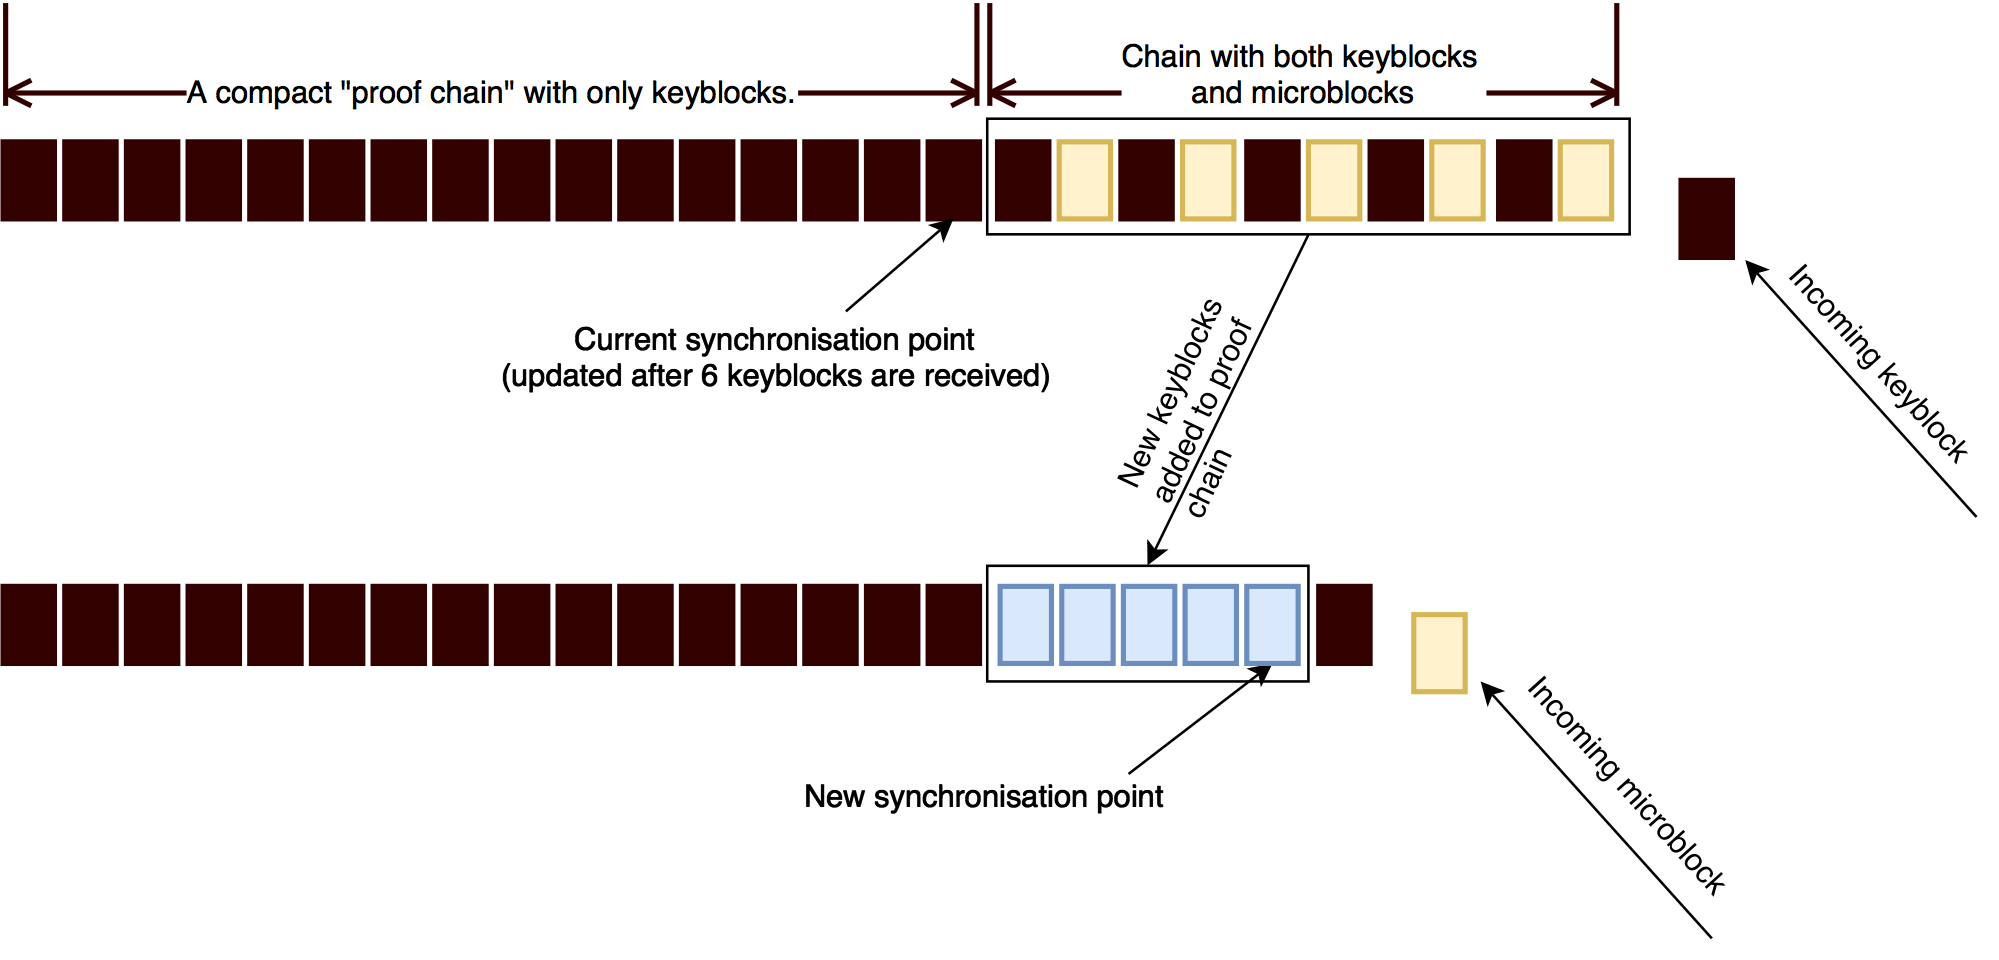
\includegraphics[width=\textwidth]{figures/sync}
    \caption{Description of how the blockchain is maintained. Each blockchain node keeps track of a window with microblock transactions for the most recent $w$ blocks on the blockchain, as well as the transactions of all keyblocks starting at the genesis block. Blockchain nodes may also keep an old copy of the account database and the account tree as they looked $w$ blocks ago, called a synchronisation point. The synchronisation point is used to bootstrap new blockchain nodes, and moves forward on a regular basis as new blocks are added to the blockchain.}
    \label{fig:sync}
\end{figure*}

\chapter{Verify a Certificate}
\label{app:verify-cert}
A client verifies a certificate by checking both the signature produced by the CA and the signature (of the public key in the certificate) produced by the domain owner. The blockchain account of the domain owner, containing the domain holder's public key, is fetched from the blockchain network or stapled in an OCSP response received from the server.

A client receives the following data (either by extracting it from a custom OCSP response or by contacting the blockchain network directly):

\begin{itemize}
    \item[\checkmark] An OID $\mathcal{K}_{\text{OID}}$ identifying the type of public key.
    \item[\checkmark] The domain holder's public key $\mathcal{K}_{S}$.
    \item[\checkmark] A block number $i$.
    \item[\checkmark] A Merkle proof $\mathcal{P}$ which proves inclusion of the domain holder's public key in block $i$.
    \item[\checkmark] A hash $H(\mathcal{A}_h)$ computed over the remaining fields in the account body.
\end{itemize}

A client synchronises and validates the block headers of the longest blockchain advertised by the network, and proceeds as follows:

\begin{enumerate}
    \item Extract the topdomain from the ``Common Name'' field of the certificate.
    \item Compute the Merkle hash of the domain holder's blockchain account as:
    \[
        H(\mathsf{topdomain} \text{ | } \mathcal{K}_{\text{OID}} \text{ | } \mathcal{K}_S \text{ | } H(\mathcal{A}_h))
    \]
    \item Use the hashes in $\mathcal{P}$ to reconstruct the Merkle root hash of the account tree for block $i$.
    \item Reject the domain holder's public key if the computed hash does not correspond to the hash found in the ``Account root hash'' field of the most recent keyblock on the blockchain.
\end{enumerate}

\end{appendices}
%%%%%%%%%%%%%%%%%%%%%%%%%%%%%%%%%%%%%%%%%%%%%%%%%%%%%%%%%%%%%%%%%%%%%%%%%%%%%%%%%%%%%%%%

\ifbook
\clearpage % flush any lingering floats

\includepdf[pages={1}]{cover/back.pdf}
\fi
\end{document}